\documentclass[twoside]{book}

% Packages required by doxygen
\usepackage{calc}
\usepackage{doxygen}
\usepackage{graphicx}
\usepackage[utf8]{inputenc}
\usepackage{makeidx}
\usepackage{multicol}
\usepackage{multirow}
\usepackage{textcomp}
\usepackage[table]{xcolor}

% Font selection
\usepackage[T1]{fontenc}
\usepackage{mathptmx}
\usepackage[scaled=.90]{helvet}
\usepackage{courier}
\usepackage{amssymb}
\usepackage{sectsty}
\renewcommand{\familydefault}{\sfdefault}
\allsectionsfont{%
  \fontseries{bc}\selectfont%
  \color{darkgray}%
}
\renewcommand{\DoxyLabelFont}{%
  \fontseries{bc}\selectfont%
  \color{darkgray}%
}

% Page & text layout
\usepackage{geometry}
\geometry{%
  a4paper,%
  top=2.5cm,%
  bottom=2.5cm,%
  left=2.5cm,%
  right=2.5cm%
}
\tolerance=750
\hfuzz=15pt
\hbadness=750
\setlength{\emergencystretch}{15pt}
\setlength{\parindent}{0cm}
\setlength{\parskip}{0.2cm}
\makeatletter
\renewcommand{\paragraph}{%
  \@startsection{paragraph}{4}{0ex}{-1.0ex}{1.0ex}{%
    \normalfont\normalsize\bfseries\SS@parafont%
  }%
}
\renewcommand{\subparagraph}{%
  \@startsection{subparagraph}{5}{0ex}{-1.0ex}{1.0ex}{%
    \normalfont\normalsize\bfseries\SS@subparafont%
  }%
}
\makeatother

% Headers & footers
\usepackage{fancyhdr}
\pagestyle{fancyplain}
\fancyhead[LE]{\fancyplain{}{\bfseries\thepage}}
\fancyhead[CE]{\fancyplain{}{}}
\fancyhead[RE]{\fancyplain{}{\bfseries\leftmark}}
\fancyhead[LO]{\fancyplain{}{\bfseries\rightmark}}
\fancyhead[CO]{\fancyplain{}{}}
\fancyhead[RO]{\fancyplain{}{\bfseries\thepage}}
\fancyfoot[LE]{\fancyplain{}{}}
\fancyfoot[CE]{\fancyplain{}{}}
\fancyfoot[RE]{\fancyplain{}{\bfseries\scriptsize Generated on Fri Nov 20 2015 09\-:57\-:46 for My Project by Doxygen }}
\fancyfoot[LO]{\fancyplain{}{\bfseries\scriptsize Generated on Fri Nov 20 2015 09\-:57\-:46 for My Project by Doxygen }}
\fancyfoot[CO]{\fancyplain{}{}}
\fancyfoot[RO]{\fancyplain{}{}}
\renewcommand{\footrulewidth}{0.4pt}
\renewcommand{\chaptermark}[1]{%
  \markboth{#1}{}%
}
\renewcommand{\sectionmark}[1]{%
  \markright{\thesection\ #1}%
}

% Indices & bibliography
\usepackage{natbib}
\usepackage[titles]{tocloft}
\setcounter{tocdepth}{3}
\setcounter{secnumdepth}{5}
\makeindex

% Hyperlinks (required, but should be loaded last)
\usepackage{ifpdf}
\ifpdf
  \usepackage[pdftex,pagebackref=true]{hyperref}
\else
  \usepackage[ps2pdf,pagebackref=true]{hyperref}
\fi
\hypersetup{%
  colorlinks=true,%
  linkcolor=blue,%
  citecolor=blue,%
  unicode%
}

% Custom commands
\newcommand{\clearemptydoublepage}{%
  \newpage{\pagestyle{empty}\cleardoublepage}%
}


%===== C O N T E N T S =====

\begin{document}

% Titlepage & ToC
\hypersetup{pageanchor=false}
\pagenumbering{roman}
\begin{titlepage}
\vspace*{7cm}
\begin{center}%
{\Large My Project }\\
\vspace*{1cm}
{\large Generated by Doxygen 1.8.6}\\
\vspace*{0.5cm}
{\small Fri Nov 20 2015 09:57:46}\\
\end{center}
\end{titlepage}
\clearemptydoublepage
\tableofcontents
\clearemptydoublepage
\pagenumbering{arabic}
\hypersetup{pageanchor=true}

%--- Begin generated contents ---
\chapter{My Personal Index Page}
\label{index}\hypertarget{index}{}\hypertarget{index_intro_sec}{}\section{Introduction}\label{index_intro_sec}
This is Dean Avery's and Kevin Wang's introduction to their iteration 3 project.\hypertarget{index_install_sec}{}\section{Installation}\label{index_install_sec}
To make our code just run make run-\/tests to execute all the tests that need to be done. 
\chapter{Hierarchical Index}
\section{Class Hierarchy}
This inheritance list is sorted roughly, but not completely, alphabetically\-:\begin{DoxyCompactList}
\item \contentsline{section}{Ext\-Token}{\pageref{classExtToken}}{}
\begin{DoxyCompactList}
\item \contentsline{section}{Char\-Const\-Token}{\pageref{classCharConstToken}}{}
\item \contentsline{section}{Dash\-Token}{\pageref{classDashToken}}{}
\item \contentsline{section}{End\-Of\-File\-Token}{\pageref{classEndOfFileToken}}{}
\item \contentsline{section}{False\-Kwd\-Token}{\pageref{classFalseKwdToken}}{}
\item \contentsline{section}{Float\-Const\-Token}{\pageref{classFloatConstToken}}{}
\item \contentsline{section}{Forward\-Slash\-Token}{\pageref{classForwardSlashToken}}{}
\item \contentsline{section}{If\-Token}{\pageref{classIfToken}}{}
\item \contentsline{section}{Int\-Const\-Token}{\pageref{classIntConstToken}}{}
\item \contentsline{section}{Left\-Paren\-Token}{\pageref{classLeftParenToken}}{}
\item \contentsline{section}{Let\-Token}{\pageref{classLetToken}}{}
\item \contentsline{section}{Not\-Op\-Token}{\pageref{classNotOpToken}}{}
\item \contentsline{section}{Plus\-Sign\-Token}{\pageref{classPlusSignToken}}{}
\item \contentsline{section}{Relational\-Op\-Token}{\pageref{classRelationalOpToken}}{}
\item \contentsline{section}{Star\-Token}{\pageref{classStarToken}}{}
\item \contentsline{section}{String\-Const\-Token}{\pageref{classStringConstToken}}{}
\item \contentsline{section}{True\-Kwd\-Token}{\pageref{classTrueKwdToken}}{}
\item \contentsline{section}{Variable\-Name\-Token}{\pageref{classVariableNameToken}}{}
\end{DoxyCompactList}
\item \contentsline{section}{Node}{\pageref{classNode}}{}
\begin{DoxyCompactList}
\item \contentsline{section}{Decl}{\pageref{classDecl}}{}
\begin{DoxyCompactList}
\item \contentsline{section}{Matrix\-Decl1}{\pageref{classMatrixDecl1}}{}
\item \contentsline{section}{Matrix\-Decl2}{\pageref{classMatrixDecl2}}{}
\item \contentsline{section}{Standard\-Decl}{\pageref{classStandardDecl}}{}
\end{DoxyCompactList}
\item \contentsline{section}{Expr}{\pageref{classExpr}}{}
\begin{DoxyCompactList}
\item \contentsline{section}{Bitwise\-Operator}{\pageref{classBitwiseOperator}}{}
\item \contentsline{section}{Const\-Expr}{\pageref{classConstExpr}}{}
\item \contentsline{section}{If\-Then\-Else\-Expr}{\pageref{classIfThenElseExpr}}{}
\item \contentsline{section}{Let\-Expr}{\pageref{classLetExpr}}{}
\item \contentsline{section}{Logic\-Operator}{\pageref{classLogicOperator}}{}
\item \contentsline{section}{Matrix\-Ref}{\pageref{classMatrixRef}}{}
\item \contentsline{section}{Nested\-Or\-Func\-Call}{\pageref{classNestedOrFuncCall}}{}
\item \contentsline{section}{Not\-Expr}{\pageref{classNotExpr}}{}
\item \contentsline{section}{Paren\-Expr}{\pageref{classParenExpr}}{}
\item \contentsline{section}{True\-Or\-False\-Expr}{\pageref{classTrueOrFalseExpr}}{}
\item \contentsline{section}{Var\-Name}{\pageref{classVarName}}{}
\end{DoxyCompactList}
\item \contentsline{section}{Program}{\pageref{classProgram}}{}
\item \contentsline{section}{Stmt}{\pageref{classStmt}}{}
\begin{DoxyCompactList}
\item \contentsline{section}{Assignment\-Matrix\-Stmt}{\pageref{classAssignmentMatrixStmt}}{}
\item \contentsline{section}{Assignment\-Stmt}{\pageref{classAssignmentStmt}}{}
\item \contentsline{section}{Curly\-Stmts}{\pageref{classCurlyStmts}}{}
\item \contentsline{section}{If\-Else\-Stmt}{\pageref{classIfElseStmt}}{}
\item \contentsline{section}{If\-Stmt}{\pageref{classIfStmt}}{}
\item \contentsline{section}{Print\-Stmt}{\pageref{classPrintStmt}}{}
\item \contentsline{section}{Repeat\-Stmt}{\pageref{classRepeatStmt}}{}
\item \contentsline{section}{Semi\-Colon\-Stmt}{\pageref{classSemiColonStmt}}{}
\item \contentsline{section}{While\-Stmt}{\pageref{classWhileStmt}}{}
\end{DoxyCompactList}
\item \contentsline{section}{Stmts}{\pageref{classStmts}}{}
\begin{DoxyCompactList}
\item \contentsline{section}{Empty\-Stmts}{\pageref{classEmptyStmts}}{}
\item \contentsline{section}{Stmt\-Stmts}{\pageref{classStmtStmts}}{}
\end{DoxyCompactList}
\end{DoxyCompactList}
\item \contentsline{section}{Parser}{\pageref{classParser}}{}
\item \contentsline{section}{Parse\-Result}{\pageref{classParseResult}}{}
\item \contentsline{section}{Scanner}{\pageref{classScanner}}{}
\item Test\-Suite\begin{DoxyCompactList}
\item \contentsline{section}{Ast\-Test\-Suite}{\pageref{classAstTestSuite}}{}
\item \contentsline{section}{Parser\-Test\-Suite}{\pageref{classParserTestSuite}}{}
\item \contentsline{section}{Regex\-Test\-Suite}{\pageref{classRegexTestSuite}}{}
\item \contentsline{section}{Scanner\-Test\-Suite}{\pageref{classScannerTestSuite}}{}
\end{DoxyCompactList}
\item \contentsline{section}{Token}{\pageref{classToken}}{}
\end{DoxyCompactList}

\chapter{Class Index}
\section{Class List}
Here are the classes, structs, unions and interfaces with brief descriptions\-:\begin{DoxyCompactList}
\item\contentsline{section}{\hyperlink{classAssignmentMatrixStmt}{Assignment\-Matrix\-Stmt} \\*\hyperlink{classStmt}{Stmt} \-:\-:= $\vert$ var\-Name '\mbox{[}' \hyperlink{classExpr}{Expr} '\-:' \hyperlink{classExpr}{Expr} '\mbox{]}' '=' \hyperlink{classExpr}{Expr} ';' matrix assignment }{\pageref{classAssignmentMatrixStmt}}{}
\item\contentsline{section}{\hyperlink{classAssignmentStmt}{Assignment\-Stmt} \\*\hyperlink{classStmt}{Stmt} \-:\-:= var\-Name '=' \hyperlink{classExpr}{Expr} ';' }{\pageref{classAssignmentStmt}}{}
\item\contentsline{section}{\hyperlink{classAstTestSuite}{Ast\-Test\-Suite} }{\pageref{classAstTestSuite}}{}
\item\contentsline{section}{\hyperlink{classBitwiseOperator}{Bitwise\-Operator} \\*Handles bitwise operators (+, -\/, $\ast$, /) }{\pageref{classBitwiseOperator}}{}
\item\contentsline{section}{\hyperlink{classCharConstToken}{Char\-Const\-Token} }{\pageref{classCharConstToken}}{}
\item\contentsline{section}{\hyperlink{classConstExpr}{Const\-Expr} \\*\hyperlink{classExpr}{Expr} \-:\-:= int\-Const $\vert$ float\-Const $\vert$ string\-Const }{\pageref{classConstExpr}}{}
\item\contentsline{section}{\hyperlink{classCurlyStmts}{Curly\-Stmts} \\*\hyperlink{classStmt}{Stmt} \-:\-:= '\{' \hyperlink{classStmts}{Stmts} '\}' This is for while loops ex\-: while (\hyperlink{classExpr}{Expr}) stmt -\/$>$ \{\hyperlink{classStmts}{Stmts}\} }{\pageref{classCurlyStmts}}{}
\item\contentsline{section}{\hyperlink{classDashToken}{Dash\-Token} }{\pageref{classDashToken}}{}
\item\contentsline{section}{\hyperlink{classDecl}{Decl} }{\pageref{classDecl}}{}
\item\contentsline{section}{\hyperlink{classEmptyStmts}{Empty\-Stmts} }{\pageref{classEmptyStmts}}{}
\item\contentsline{section}{\hyperlink{classEndOfFileToken}{End\-Of\-File\-Token} }{\pageref{classEndOfFileToken}}{}
\item\contentsline{section}{\hyperlink{classExpr}{Expr} }{\pageref{classExpr}}{}
\item\contentsline{section}{\hyperlink{classExtToken}{Ext\-Token} }{\pageref{classExtToken}}{}
\item\contentsline{section}{\hyperlink{classFalseKwdToken}{False\-Kwd\-Token} }{\pageref{classFalseKwdToken}}{}
\item\contentsline{section}{\hyperlink{classFloatConstToken}{Float\-Const\-Token} }{\pageref{classFloatConstToken}}{}
\item\contentsline{section}{\hyperlink{classForwardSlashToken}{Forward\-Slash\-Token} }{\pageref{classForwardSlashToken}}{}
\item\contentsline{section}{\hyperlink{classIfElseStmt}{If\-Else\-Stmt} \\*\hyperlink{classStmt}{Stmt} \-:\-:= 'if' '(' \hyperlink{classExpr}{Expr} ')' \hyperlink{classStmt}{Stmt} 'else' \hyperlink{classStmt}{Stmt} }{\pageref{classIfElseStmt}}{}
\item\contentsline{section}{\hyperlink{classIfStmt}{If\-Stmt} \\*\hyperlink{classStmt}{Stmt}\-:\-:= 'if' '('\hyperlink{classExpr}{Expr}')' \hyperlink{classStmt}{Stmt} }{\pageref{classIfStmt}}{}
\item\contentsline{section}{\hyperlink{classIfThenElseExpr}{If\-Then\-Else\-Expr} \\*\hyperlink{classExpr}{Expr} \-:\-:= 'if' \hyperlink{classExpr}{Expr} 'then' \hyperlink{classExpr}{Expr} 'else' \hyperlink{classExpr}{Expr} //\-If\-Expr }{\pageref{classIfThenElseExpr}}{}
\item\contentsline{section}{\hyperlink{classIfToken}{If\-Token} }{\pageref{classIfToken}}{}
\item\contentsline{section}{\hyperlink{classIntConstToken}{Int\-Const\-Token} }{\pageref{classIntConstToken}}{}
\item\contentsline{section}{\hyperlink{classLeftParenToken}{Left\-Paren\-Token} }{\pageref{classLeftParenToken}}{}
\item\contentsline{section}{\hyperlink{classLetExpr}{Let\-Expr} \\*\hyperlink{classExpr}{Expr} \-:\-:= 'let' \hyperlink{classStmts}{Stmts} 'in' \hyperlink{classExpr}{Expr} 'end' //\-Let\-Expr }{\pageref{classLetExpr}}{}
\item\contentsline{section}{\hyperlink{classLetToken}{Let\-Token} }{\pageref{classLetToken}}{}
\item\contentsline{section}{\hyperlink{classLogicOperator}{Logic\-Operator} \\*Handles logic operators ($>$, $>$=, $<$, $<$=, ==, !=, \&\&, $\vert$$\vert$) }{\pageref{classLogicOperator}}{}
\item\contentsline{section}{\hyperlink{classMatrixDecl1}{Matrix\-Decl1} \\*\hyperlink{classDecl}{Decl} \-:\-:= 'matrix' var\-Name '\mbox{[}' \hyperlink{classExpr}{Expr} '\-:' \hyperlink{classExpr}{Expr} '\mbox{]}' var\-Name '\-:' var\-Name '=' \hyperlink{classExpr}{Expr} ';' }{\pageref{classMatrixDecl1}}{}
\item\contentsline{section}{\hyperlink{classMatrixDecl2}{Matrix\-Decl2} \\*\hyperlink{classDecl}{Decl} \-:\-:= 'matrix' var\-Name '=' \hyperlink{classExpr}{Expr} ';' }{\pageref{classMatrixDecl2}}{}
\item\contentsline{section}{\hyperlink{classMatrixRef}{Matrix\-Ref} \\*\hyperlink{classExpr}{Expr} \-:\-:= var\-Name '\mbox{[}' \hyperlink{classExpr}{Expr} '\-:' \hyperlink{classExpr}{Expr} '\mbox{]}' //\-Matrix\-R\-Ef }{\pageref{classMatrixRef}}{}
\item\contentsline{section}{\hyperlink{classNestedOrFuncCall}{Nested\-Or\-Func\-Call} \\*\hyperlink{classExpr}{Expr} \-:\-:= var\-Name '(' \hyperlink{classExpr}{Expr} ')' //\-Nested\-Or\-Function\-Call }{\pageref{classNestedOrFuncCall}}{}
\item\contentsline{section}{\hyperlink{classNode}{Node} \\*\hyperlink{classNode}{Node} }{\pageref{classNode}}{}
\item\contentsline{section}{\hyperlink{classNotExpr}{Not\-Expr} \\*\hyperlink{classExpr}{Expr} \-:\-:= '!' \hyperlink{classExpr}{Expr} }{\pageref{classNotExpr}}{}
\item\contentsline{section}{\hyperlink{classNotOpToken}{Not\-Op\-Token} }{\pageref{classNotOpToken}}{}
\item\contentsline{section}{\hyperlink{classParenExpr}{Paren\-Expr} \\*\hyperlink{classExpr}{Expr} \-:\-:= '(' \hyperlink{classExpr}{Expr} ')' }{\pageref{classParenExpr}}{}
\item\contentsline{section}{\hyperlink{classParser}{Parser} }{\pageref{classParser}}{}
\item\contentsline{section}{\hyperlink{classParseResult}{Parse\-Result} }{\pageref{classParseResult}}{}
\item\contentsline{section}{\hyperlink{classParserTestSuite}{Parser\-Test\-Suite} }{\pageref{classParserTestSuite}}{}
\item\contentsline{section}{\hyperlink{classPlusSignToken}{Plus\-Sign\-Token} }{\pageref{classPlusSignToken}}{}
\item\contentsline{section}{\hyperlink{classPrintStmt}{Print\-Stmt} \\*\hyperlink{classStmt}{Stmt} \-:\-:= 'print' '(' \hyperlink{classExpr}{Expr} ')' ';' }{\pageref{classPrintStmt}}{}
\item\contentsline{section}{\hyperlink{classProgram}{Program} \\*\hyperlink{classProgram}{Program} \-:\-:= var\-Name '(' ')' '\{' \hyperlink{classStmts}{Stmts} '\}' }{\pageref{classProgram}}{}
\item\contentsline{section}{\hyperlink{classRegexTestSuite}{Regex\-Test\-Suite} }{\pageref{classRegexTestSuite}}{}
\item\contentsline{section}{\hyperlink{classRelationalOpToken}{Relational\-Op\-Token} }{\pageref{classRelationalOpToken}}{}
\item\contentsline{section}{\hyperlink{classRepeatStmt}{Repeat\-Stmt} \\*\hyperlink{classStmt}{Stmt} \-:\-:= 'repeat' '(' var\-Name '=' \hyperlink{classExpr}{Expr} 'to' \hyperlink{classExpr}{Expr} ')' \hyperlink{classStmt}{Stmt} }{\pageref{classRepeatStmt}}{}
\item\contentsline{section}{\hyperlink{classScanner}{Scanner} }{\pageref{classScanner}}{}
\item\contentsline{section}{\hyperlink{classScannerTestSuite}{Scanner\-Test\-Suite} }{\pageref{classScannerTestSuite}}{}
\item\contentsline{section}{\hyperlink{classSemiColonStmt}{Semi\-Colon\-Stmt} \\*\hyperlink{classStmt}{Stmt} \-:\-:= ';' }{\pageref{classSemiColonStmt}}{}
\item\contentsline{section}{\hyperlink{classStandardDecl}{Standard\-Decl} \\*\hyperlink{classDecl}{Decl} \-:\-:= integer\-Kwd var\-Name $\vert$ float\-Kwd var\-Name $\vert$ string\-Kwd var\-Name $\vert$ bool\-Kwd var\-Name }{\pageref{classStandardDecl}}{}
\item\contentsline{section}{\hyperlink{classStarToken}{Star\-Token} }{\pageref{classStarToken}}{}
\item\contentsline{section}{\hyperlink{classStmt}{Stmt} }{\pageref{classStmt}}{}
\item\contentsline{section}{\hyperlink{classStmts}{Stmts} }{\pageref{classStmts}}{}
\item\contentsline{section}{\hyperlink{classStmtStmts}{Stmt\-Stmts} }{\pageref{classStmtStmts}}{}
\item\contentsline{section}{\hyperlink{classStringConstToken}{String\-Const\-Token} }{\pageref{classStringConstToken}}{}
\item\contentsline{section}{\hyperlink{classToken}{Token} }{\pageref{classToken}}{}
\item\contentsline{section}{\hyperlink{classTrueKwdToken}{True\-Kwd\-Token} }{\pageref{classTrueKwdToken}}{}
\item\contentsline{section}{\hyperlink{classTrueOrFalseExpr}{True\-Or\-False\-Expr} \\*\hyperlink{classExpr}{Expr} \-:\-:= 'true' $\vert$ 'false' }{\pageref{classTrueOrFalseExpr}}{}
\item\contentsline{section}{\hyperlink{classVariableNameToken}{Variable\-Name\-Token} }{\pageref{classVariableNameToken}}{}
\item\contentsline{section}{\hyperlink{classVarName}{Var\-Name} \\*The \hyperlink{classVarName}{Var\-Name} constructor is passed the string name from prev\-Token-\/$>$lexeme }{\pageref{classVarName}}{}
\item\contentsline{section}{\hyperlink{classWhileStmt}{While\-Stmt} \\*\hyperlink{classStmt}{Stmt} \-:\-:= 'while' '(' \hyperlink{classExpr}{Expr} ')' \hyperlink{classStmt}{Stmt} }{\pageref{classWhileStmt}}{}
\end{DoxyCompactList}

\chapter{Class Documentation}
\hypertarget{classAssignmentMatrixStmt}{\section{Assignment\-Matrix\-Stmt Class Reference}
\label{classAssignmentMatrixStmt}\index{Assignment\-Matrix\-Stmt@{Assignment\-Matrix\-Stmt}}
}


\hyperlink{classStmt}{Stmt} \-:\-:= $\vert$ var\-Name '\mbox{[}' \hyperlink{classExpr}{Expr} '\-:' \hyperlink{classExpr}{Expr} '\mbox{]}' '=' \hyperlink{classExpr}{Expr} ';' matrix assignment.  




{\ttfamily \#include $<$A\-S\-T.\-h$>$}

Inheritance diagram for Assignment\-Matrix\-Stmt\-:\begin{figure}[H]
\begin{center}
\leavevmode
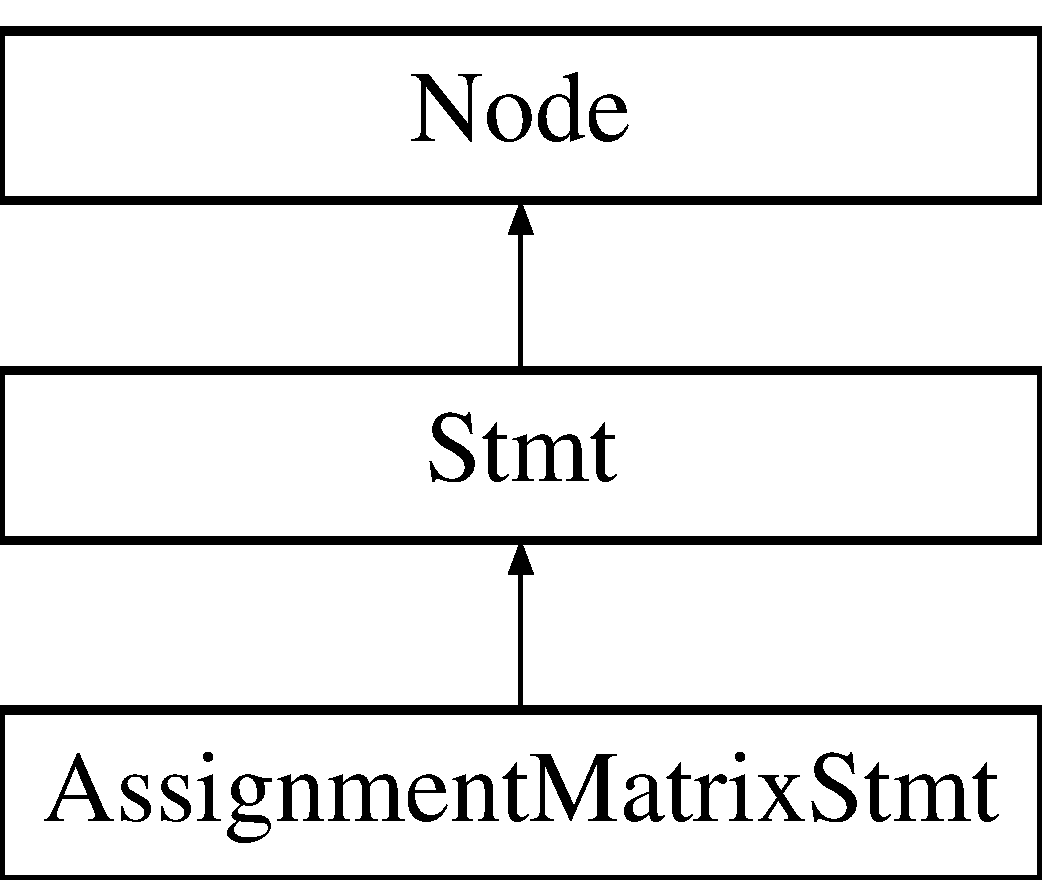
\includegraphics[height=3.000000cm]{classAssignmentMatrixStmt}
\end{center}
\end{figure}
\subsection*{Public Member Functions}
\begin{DoxyCompactItemize}
\item 
\hypertarget{classAssignmentMatrixStmt_a203671ccddaeef9edac2834b8db3b423}{{\bfseries Assignment\-Matrix\-Stmt} (std\-::string v, \hyperlink{classExpr}{Expr} $\ast$e1, \hyperlink{classExpr}{Expr} $\ast$e2, \hyperlink{classExpr}{Expr} $\ast$e3)}\label{classAssignmentMatrixStmt_a203671ccddaeef9edac2834b8db3b423}

\item 
\hypertarget{classAssignmentMatrixStmt_adbdf4dee03753d6a0a098cf3a9eff6a8}{std\-::string \hyperlink{classAssignmentMatrixStmt_adbdf4dee03753d6a0a098cf3a9eff6a8}{unparse} ()}\label{classAssignmentMatrixStmt_adbdf4dee03753d6a0a098cf3a9eff6a8}

\begin{DoxyCompactList}\small\item\em Unparse in proper 'matrix assignment' form as denoted in grammar. \end{DoxyCompactList}\end{DoxyCompactItemize}


\subsection{Detailed Description}
\hyperlink{classStmt}{Stmt} \-:\-:= $\vert$ var\-Name '\mbox{[}' \hyperlink{classExpr}{Expr} '\-:' \hyperlink{classExpr}{Expr} '\mbox{]}' '=' \hyperlink{classExpr}{Expr} ';' matrix assignment. 

The documentation for this class was generated from the following file\-:\begin{DoxyCompactItemize}
\item 
A\-S\-T.\-h\end{DoxyCompactItemize}

\hypertarget{classAssignmentStmt}{\section{Assignment\-Stmt Class Reference}
\label{classAssignmentStmt}\index{Assignment\-Stmt@{Assignment\-Stmt}}
}


\hyperlink{classStmt}{Stmt} \-:\-:= var\-Name '=' \hyperlink{classExpr}{Expr} ';'.  




{\ttfamily \#include $<$A\-S\-T.\-h$>$}

Inheritance diagram for Assignment\-Stmt\-:\begin{figure}[H]
\begin{center}
\leavevmode
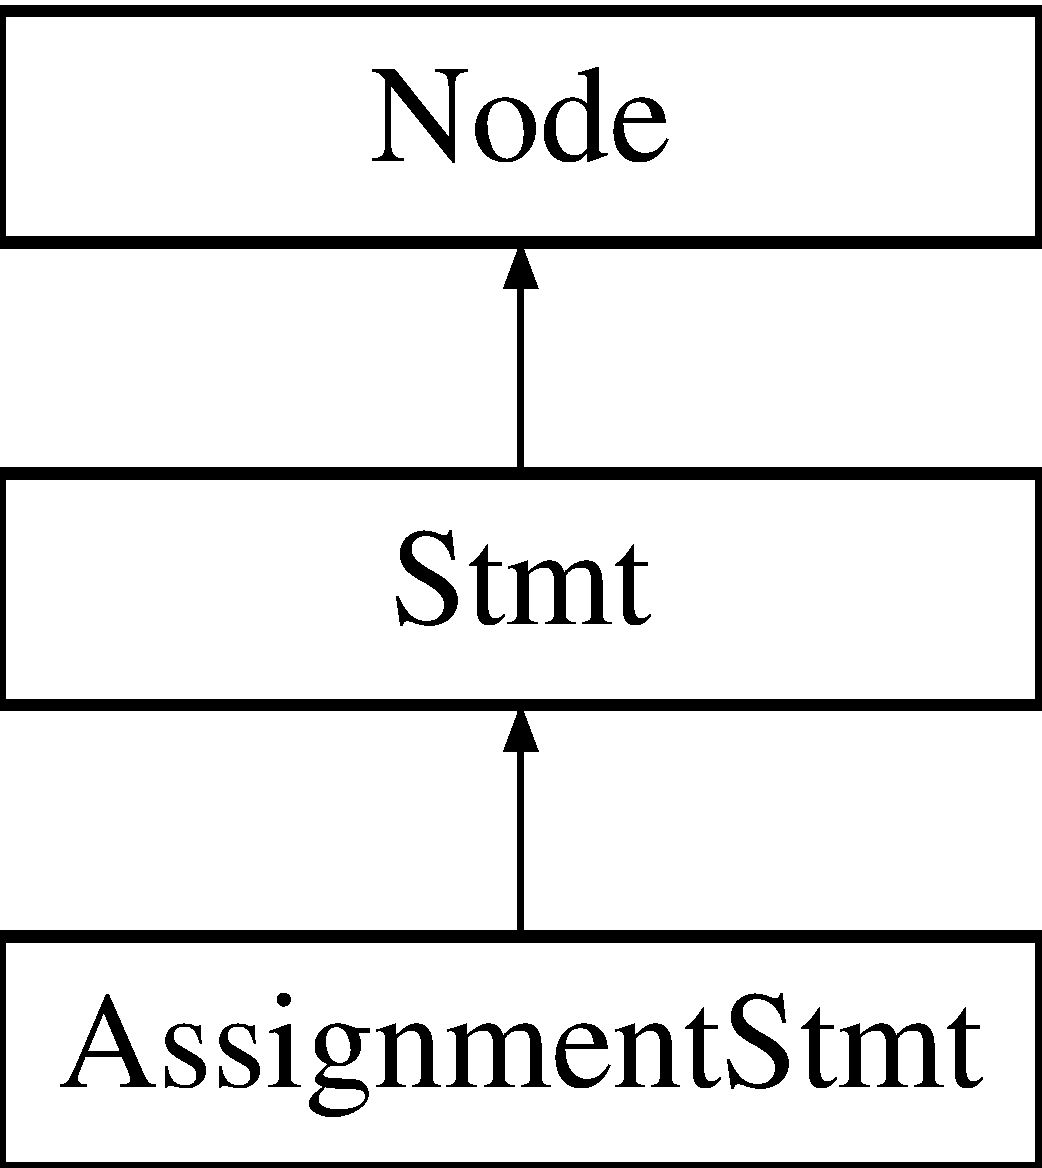
\includegraphics[height=3.000000cm]{classAssignmentStmt}
\end{center}
\end{figure}
\subsection*{Public Member Functions}
\begin{DoxyCompactItemize}
\item 
\hypertarget{classAssignmentStmt_a17759045b340d16902f645dc617f2a5e}{{\bfseries Assignment\-Stmt} (std\-::string v, \hyperlink{classExpr}{Expr} $\ast$e)}\label{classAssignmentStmt_a17759045b340d16902f645dc617f2a5e}

\item 
\hypertarget{classAssignmentStmt_a892c33dd7fa55fda0f85ced1b5684f98}{std\-::string \hyperlink{classAssignmentStmt_a892c33dd7fa55fda0f85ced1b5684f98}{unparse} ()}\label{classAssignmentStmt_a892c33dd7fa55fda0f85ced1b5684f98}

\begin{DoxyCompactList}\small\item\em Unparse in format "var\-Name = 'Expression const';. \end{DoxyCompactList}\end{DoxyCompactItemize}


\subsection{Detailed Description}
\hyperlink{classStmt}{Stmt} \-:\-:= var\-Name '=' \hyperlink{classExpr}{Expr} ';'. 

The documentation for this class was generated from the following file\-:\begin{DoxyCompactItemize}
\item 
A\-S\-T.\-h\end{DoxyCompactItemize}

\hypertarget{classAstTestSuite}{\section{Ast\-Test\-Suite Class Reference}
\label{classAstTestSuite}\index{Ast\-Test\-Suite@{Ast\-Test\-Suite}}
}
Inheritance diagram for Ast\-Test\-Suite\-:\begin{figure}[H]
\begin{center}
\leavevmode
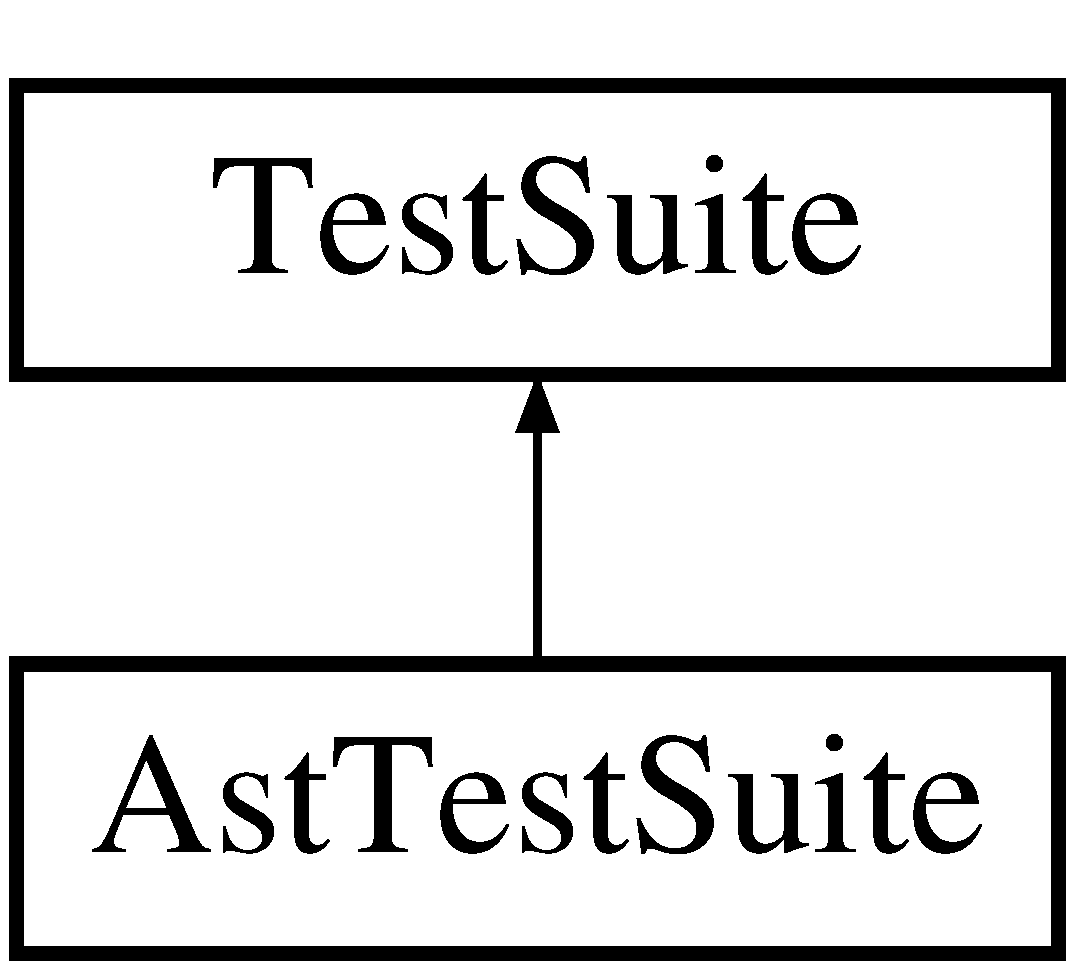
\includegraphics[height=2.000000cm]{classAstTestSuite}
\end{center}
\end{figure}
\subsection*{Public Member Functions}
\begin{DoxyCompactItemize}
\item 
\hypertarget{classAstTestSuite_a2f0462e7a965acda10e09e70432cab40}{char $\ast$$\ast$ {\bfseries make\-Args} (const char $\ast$a0, const char $\ast$a1)}\label{classAstTestSuite_a2f0462e7a965acda10e09e70432cab40}

\item 
\hypertarget{classAstTestSuite_ab935b3c95647b24b5f250b7e3332a313}{void {\bfseries write\-File} (const string text, const string filename)}\label{classAstTestSuite_ab935b3c95647b24b5f250b7e3332a313}

\item 
\hypertarget{classAstTestSuite_afb1462e2494b011f0e5077a567e0ba3d}{char $\ast$ {\bfseries read\-File} (const char $\ast$fn)}\label{classAstTestSuite_afb1462e2494b011f0e5077a567e0ba3d}

\item 
void \hyperlink{classAstTestSuite_a1fb6dcbf82548632381eb89079b456aa}{unparse\-\_\-tests} (string file)
\item 
void \hyperlink{classAstTestSuite_a3d75ff50ddf8e97bd5ad96751dc0df5b}{xtest\-\_\-iter3\-\_\-simple1} (void)
\begin{DoxyCompactList}\small\item\em S\-I\-M\-P\-L\-E T\-E\-S\-T\-S A\-D\-D\-E\-D B\-Y D\-E\-A\-N. \end{DoxyCompactList}\item 
\hypertarget{classAstTestSuite_a9fb3d77a673b94cf2788624cba9ba004}{void {\bfseries xtest\-\_\-iter3\-\_\-simple2} (void)}\label{classAstTestSuite_a9fb3d77a673b94cf2788624cba9ba004}

\item 
\hypertarget{classAstTestSuite_a8d893b852eee4ae321357a240171857e}{void {\bfseries xtest\-\_\-iter3\-\_\-simple3} (void)}\label{classAstTestSuite_a8d893b852eee4ae321357a240171857e}

\item 
\hypertarget{classAstTestSuite_ade48304a65cbc7449bd22ec9097b6a8c}{void {\bfseries test\-\_\-sample\-\_\-1} (void)}\label{classAstTestSuite_ade48304a65cbc7449bd22ec9097b6a8c}

\item 
\hypertarget{classAstTestSuite_af764267aa9a94610fd5307ae81107312}{void {\bfseries test\-\_\-sample\-\_\-2} (void)}\label{classAstTestSuite_af764267aa9a94610fd5307ae81107312}

\item 
\hypertarget{classAstTestSuite_a956750fe55d2eb218eb75bd7dc75bc34}{void {\bfseries test\-\_\-sample\-\_\-3} (void)}\label{classAstTestSuite_a956750fe55d2eb218eb75bd7dc75bc34}

\item 
\hypertarget{classAstTestSuite_a665836b3d23c82eda3233a3c5d2f0ba4}{void {\bfseries test\-\_\-sample\-\_\-4} (void)}\label{classAstTestSuite_a665836b3d23c82eda3233a3c5d2f0ba4}

\item 
\hypertarget{classAstTestSuite_a9cceb7f0e5a6714d539f25db38424851}{void {\bfseries test\-\_\-sample\-\_\-5} (void)}\label{classAstTestSuite_a9cceb7f0e5a6714d539f25db38424851}

\item 
\hypertarget{classAstTestSuite_adbc7de61740aaf9ebf9b7e25f024f318}{void {\bfseries test\-\_\-mysample} (void)}\label{classAstTestSuite_adbc7de61740aaf9ebf9b7e25f024f318}

\item 
\hypertarget{classAstTestSuite_ade9231acfe5f8c8f02e00e54749cf99b}{void {\bfseries test\-\_\-forest\-\_\-loss} (void)}\label{classAstTestSuite_ade9231acfe5f8c8f02e00e54749cf99b}

\item 
\hypertarget{classAstTestSuite_a16655184424f2e2ca15b5110a6f9350f}{void {\bfseries xtest\-\_\-sample\-\_\-6} (void)}\label{classAstTestSuite_a16655184424f2e2ca15b5110a6f9350f}

\end{DoxyCompactItemize}
\subsection*{Public Attributes}
\begin{DoxyCompactItemize}
\item 
\hypertarget{classAstTestSuite_a148a26ab78abac732d857d7095f6dea5}{\hyperlink{classParser}{Parser} {\bfseries p}}\label{classAstTestSuite_a148a26ab78abac732d857d7095f6dea5}

\item 
\hypertarget{classAstTestSuite_ab27964f1743a2889538ca27e644eb1aa}{\hyperlink{classParseResult}{Parse\-Result} {\bfseries pr}}\label{classAstTestSuite_ab27964f1743a2889538ca27e644eb1aa}

\end{DoxyCompactItemize}


\subsection{Member Function Documentation}
\hypertarget{classAstTestSuite_a1fb6dcbf82548632381eb89079b456aa}{\index{Ast\-Test\-Suite@{Ast\-Test\-Suite}!unparse\-\_\-tests@{unparse\-\_\-tests}}
\index{unparse\-\_\-tests@{unparse\-\_\-tests}!AstTestSuite@{Ast\-Test\-Suite}}
\subsubsection[{unparse\-\_\-tests}]{\setlength{\rightskip}{0pt plus 5cm}void Ast\-Test\-Suite\-::unparse\-\_\-tests (
\begin{DoxyParamCaption}
\item[{string}]{file}
\end{DoxyParamCaption}
)\hspace{0.3cm}{\ttfamily [inline]}}}\label{classAstTestSuite_a1fb6dcbf82548632381eb89079b456aa}

\begin{DoxyEnumerate}
\item Test that the file can be parsed.
\item Verify that the ast field is not null
\item Verify that the \char`\"{}unparsing\char`\"{} is non-\/empty.
\item Verify that the un-\/parsed string can be parsed.
\item Verify that the ast field is not null after first unparsing
\item Verify that this second unparsing can be parsed.
\item Verify that the first and second unparsings are the same.
\item Verifty that the second and third unparsings are the same. 
\end{DoxyEnumerate}\hypertarget{classAstTestSuite_a3d75ff50ddf8e97bd5ad96751dc0df5b}{\index{Ast\-Test\-Suite@{Ast\-Test\-Suite}!xtest\-\_\-iter3\-\_\-simple1@{xtest\-\_\-iter3\-\_\-simple1}}
\index{xtest\-\_\-iter3\-\_\-simple1@{xtest\-\_\-iter3\-\_\-simple1}!AstTestSuite@{Ast\-Test\-Suite}}
\subsubsection[{xtest\-\_\-iter3\-\_\-simple1}]{\setlength{\rightskip}{0pt plus 5cm}void Ast\-Test\-Suite\-::xtest\-\_\-iter3\-\_\-simple1 (
\begin{DoxyParamCaption}
\item[{void}]{}
\end{DoxyParamCaption}
)\hspace{0.3cm}{\ttfamily [inline]}}}\label{classAstTestSuite_a3d75ff50ddf8e97bd5ad96751dc0df5b}


S\-I\-M\-P\-L\-E T\-E\-S\-T\-S A\-D\-D\-E\-D B\-Y D\-E\-A\-N. 

The approximate order in which the tests were implemented and passed\-: \subsubsection*{I\-M\-P\-L\-E\-M\-E\-N\-T\-E\-D P\-A\-S\-S\-E\-D }

1) test\-\_\-iter3\-\_\-simple1 11/8/15 11/8/15 2) test\-\_\-mysample 11/8/15 11/8/15 3) test\-\_\-iter3\-\_\-simple2 11/8/15 11/10/15 4) test\-\_\-sample\-\_\-1 11/9/15 11/10/15 5) test\-\_\-iter3\-\_\-simple3 11/9/15 11/11/15 6) test\-\_\-sample\-\_\-2 11/10/15 11/11/15 7) test\-\_\-sample\-\_\-3 11/11/15 11/11/15 8) test\-\_\-sample\-\_\-4 11/11/15 11/11/15 9) test\-\_\-sample\-\_\-5 11/11/15 11/12/15 10) test\-\_\-forest\-\_\-loss 11/12/15 11/12/15 11) test\-\_\-sample\-\_\-6 11/12/15 11/12/15 

The documentation for this class was generated from the following file\-:\begin{DoxyCompactItemize}
\item 
ast\-\_\-tests.\-h\end{DoxyCompactItemize}

\hypertarget{classBitwiseOperator}{\section{Bitwise\-Operator Class Reference}
\label{classBitwiseOperator}\index{Bitwise\-Operator@{Bitwise\-Operator}}
}


Handles bitwise operators (+, -\/, $\ast$, /)  




{\ttfamily \#include $<$A\-S\-T.\-h$>$}

Inheritance diagram for Bitwise\-Operator\-:\begin{figure}[H]
\begin{center}
\leavevmode
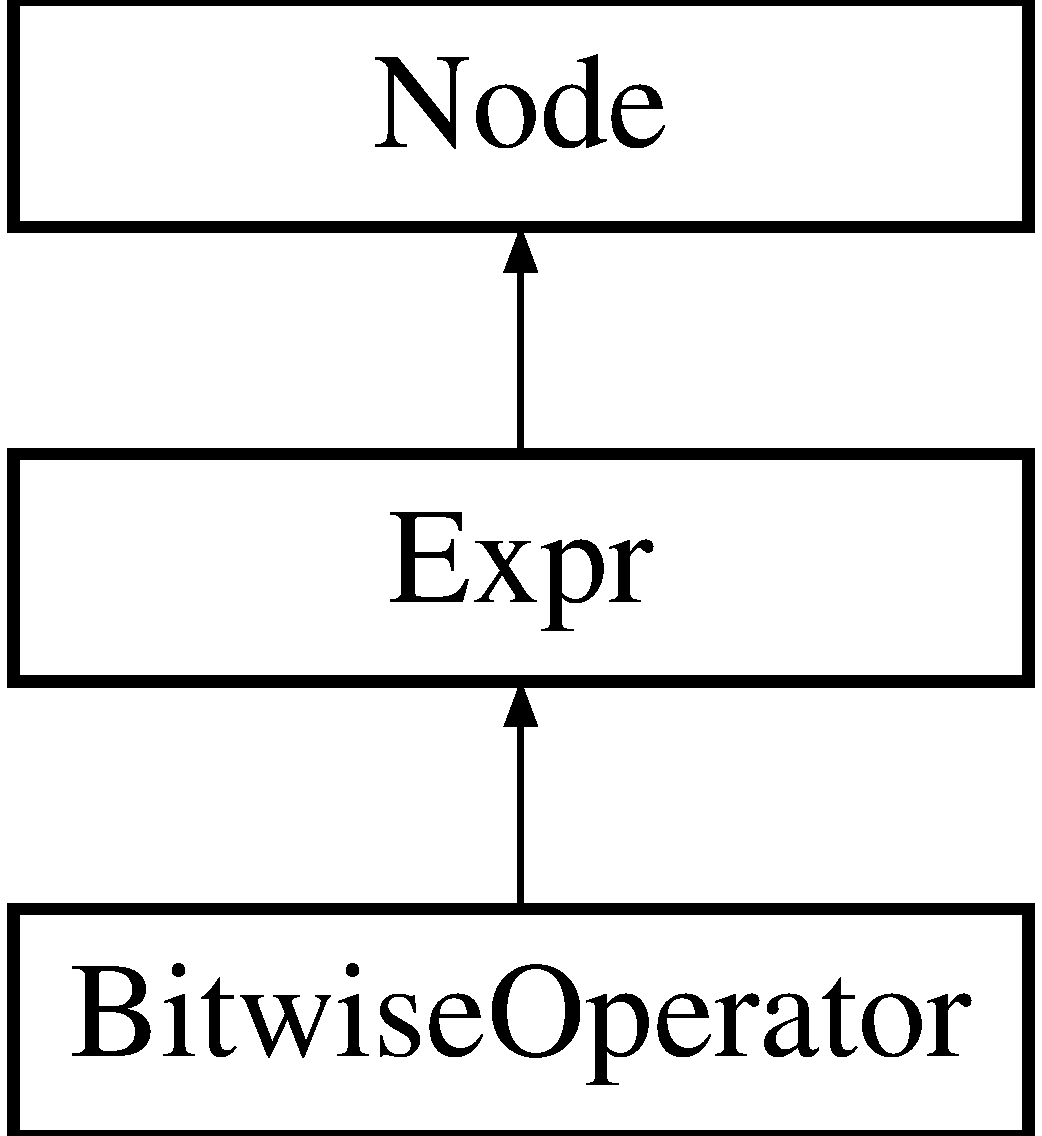
\includegraphics[height=3.000000cm]{classBitwiseOperator}
\end{center}
\end{figure}
\subsection*{Public Member Functions}
\begin{DoxyCompactItemize}
\item 
\hypertarget{classBitwiseOperator_ab8e77f532c44d54982359db0a5a549d2}{{\bfseries Bitwise\-Operator} (\hyperlink{classExpr}{Expr} $\ast$e1, std\-::string op, \hyperlink{classExpr}{Expr} $\ast$e2)}\label{classBitwiseOperator_ab8e77f532c44d54982359db0a5a549d2}

\item 
\hypertarget{classBitwiseOperator_aab4c8032951100835bdcebf08e924e5e}{std\-::string \hyperlink{classBitwiseOperator_aab4c8032951100835bdcebf08e924e5e}{unparse} ()}\label{classBitwiseOperator_aab4c8032951100835bdcebf08e924e5e}

\begin{DoxyCompactList}\small\item\em Unparse expression one and expression two separated by the proper bitwise operator. \end{DoxyCompactList}\end{DoxyCompactItemize}


\subsection{Detailed Description}
Handles bitwise operators (+, -\/, $\ast$, /) 

The documentation for this class was generated from the following file\-:\begin{DoxyCompactItemize}
\item 
A\-S\-T.\-h\end{DoxyCompactItemize}

\hypertarget{classCharConstToken}{\section{Char\-Const\-Token Class Reference}
\label{classCharConstToken}\index{Char\-Const\-Token@{Char\-Const\-Token}}
}
Inheritance diagram for Char\-Const\-Token\-:\begin{figure}[H]
\begin{center}
\leavevmode
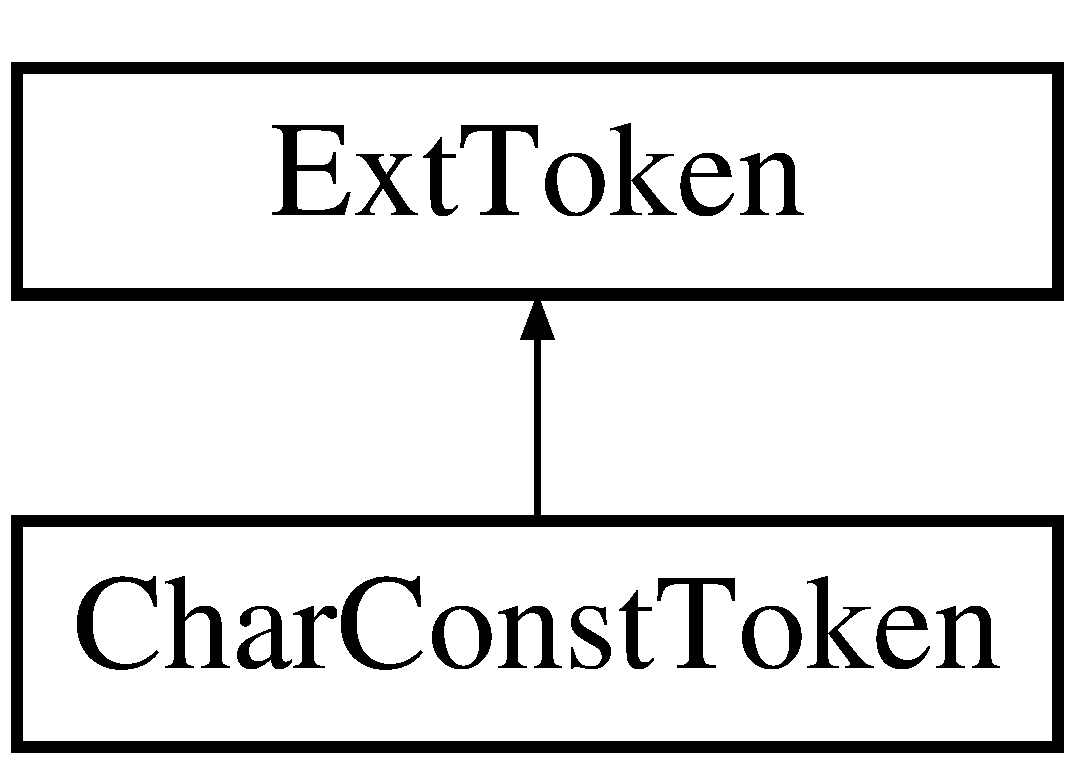
\includegraphics[height=2.000000cm]{classCharConstToken}
\end{center}
\end{figure}
\subsection*{Public Member Functions}
\begin{DoxyCompactItemize}
\item 
\hypertarget{classCharConstToken_a9dcb8d0d26c4f9c66570357641933c51}{{\bfseries Char\-Const\-Token} (\hyperlink{classParser}{Parser} $\ast$p, \hyperlink{classToken}{Token} $\ast$t)}\label{classCharConstToken_a9dcb8d0d26c4f9c66570357641933c51}

\item 
\hypertarget{classCharConstToken_a33032d6b35ef2b6ebc4db770b374ad5b}{\hyperlink{classParseResult}{Parse\-Result} {\bfseries nud} ()}\label{classCharConstToken_a33032d6b35ef2b6ebc4db770b374ad5b}

\item 
\hypertarget{classCharConstToken_addf2603d51bc2be908137f06737d8b30}{std\-::string {\bfseries description} ()}\label{classCharConstToken_addf2603d51bc2be908137f06737d8b30}

\end{DoxyCompactItemize}
\subsection*{Additional Inherited Members}


The documentation for this class was generated from the following file\-:\begin{DoxyCompactItemize}
\item 
ext\-Token.\-h\end{DoxyCompactItemize}

\hypertarget{classConstExpr}{\section{Const\-Expr Class Reference}
\label{classConstExpr}\index{Const\-Expr@{Const\-Expr}}
}


\hyperlink{classExpr}{Expr} \-:\-:= int\-Const $\vert$ float\-Const $\vert$ string\-Const.  




{\ttfamily \#include $<$A\-S\-T.\-h$>$}

Inheritance diagram for Const\-Expr\-:\begin{figure}[H]
\begin{center}
\leavevmode
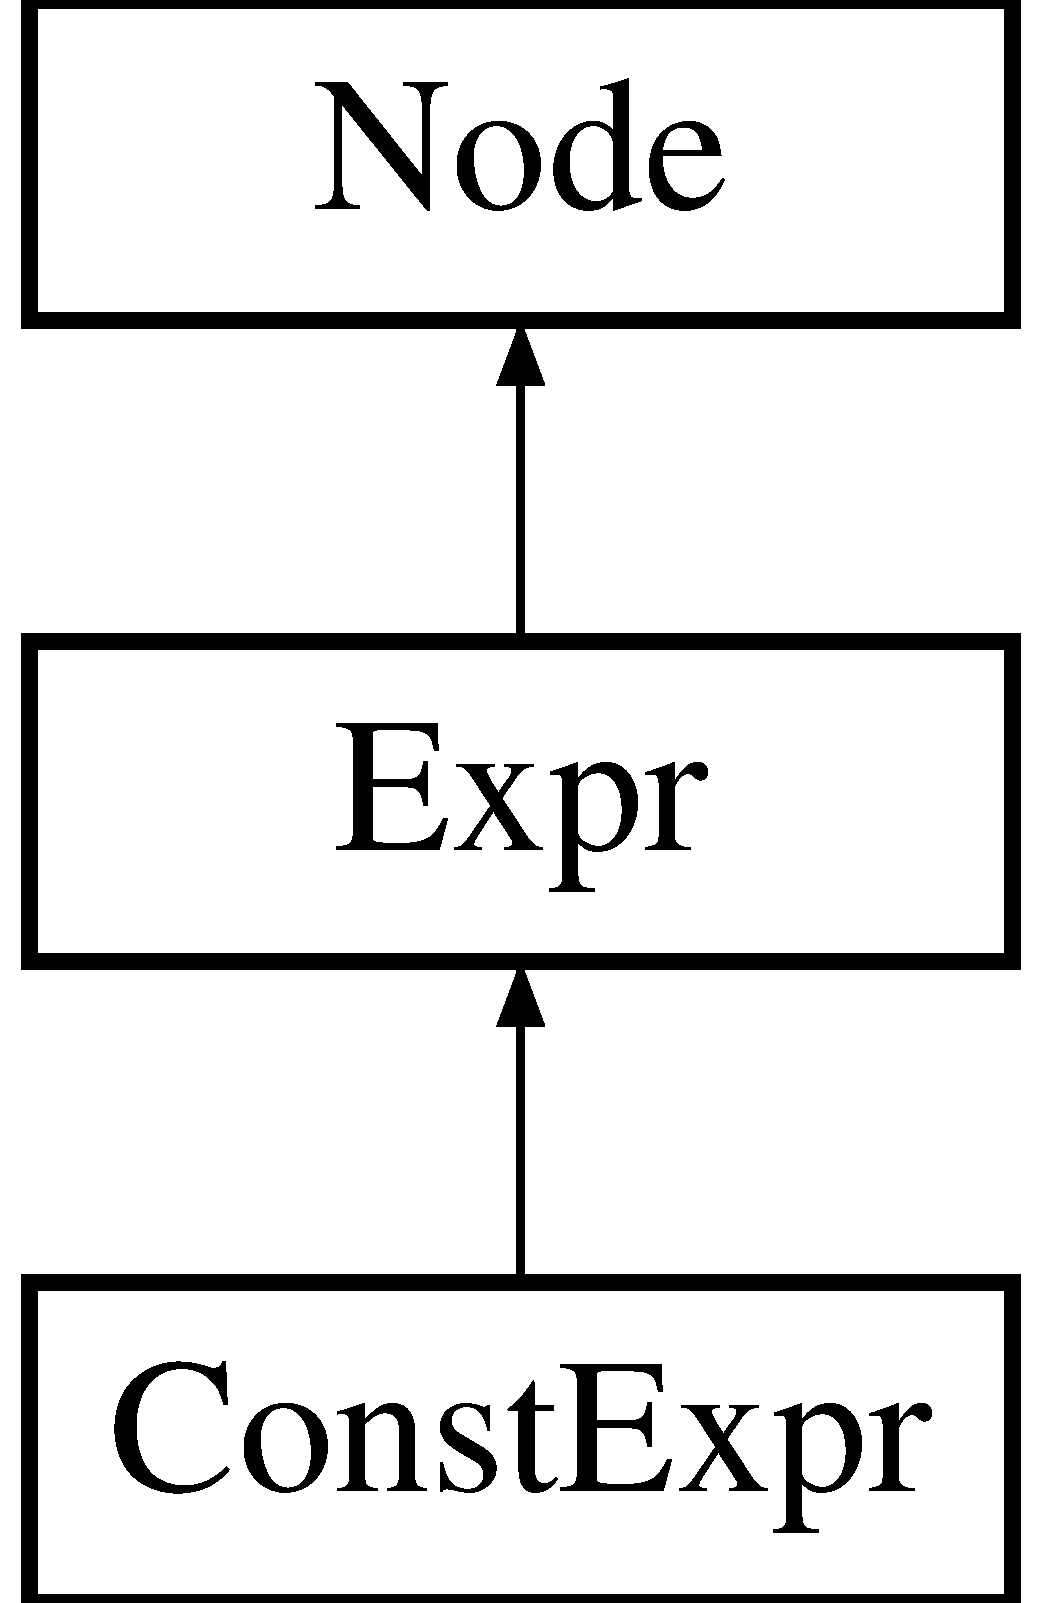
\includegraphics[height=3.000000cm]{classConstExpr}
\end{center}
\end{figure}
\subsection*{Public Member Functions}
\begin{DoxyCompactItemize}
\item 
\hypertarget{classConstExpr_a043e22c04b62fc8087e3309292475ee2}{{\bfseries Const\-Expr} (std\-::string cs)}\label{classConstExpr_a043e22c04b62fc8087e3309292475ee2}

\item 
\hypertarget{classConstExpr_adc01f00000a931c663aedffdfcd132ad}{std\-::string \hyperlink{classConstExpr_adc01f00000a931c663aedffdfcd132ad}{unparse} ()}\label{classConstExpr_adc01f00000a931c663aedffdfcd132ad}

\begin{DoxyCompactList}\small\item\em Unparse the integer\-Const $\vert$ float\-Const $\vert$ string\-Const as a string. \end{DoxyCompactList}\end{DoxyCompactItemize}


\subsection{Detailed Description}
\hyperlink{classExpr}{Expr} \-:\-:= int\-Const $\vert$ float\-Const $\vert$ string\-Const. 

The documentation for this class was generated from the following file\-:\begin{DoxyCompactItemize}
\item 
A\-S\-T.\-h\end{DoxyCompactItemize}

\hypertarget{classCurlyStmts}{\section{Curly\-Stmts Class Reference}
\label{classCurlyStmts}\index{Curly\-Stmts@{Curly\-Stmts}}
}


\hyperlink{classStmt}{Stmt} \-:\-:= '\{' \hyperlink{classStmts}{Stmts} '\}' This is for while loops ex\-: while (\hyperlink{classExpr}{Expr}) stmt -\/$>$ \{\hyperlink{classStmts}{Stmts}\}.  




{\ttfamily \#include $<$A\-S\-T.\-h$>$}

Inheritance diagram for Curly\-Stmts\-:\begin{figure}[H]
\begin{center}
\leavevmode
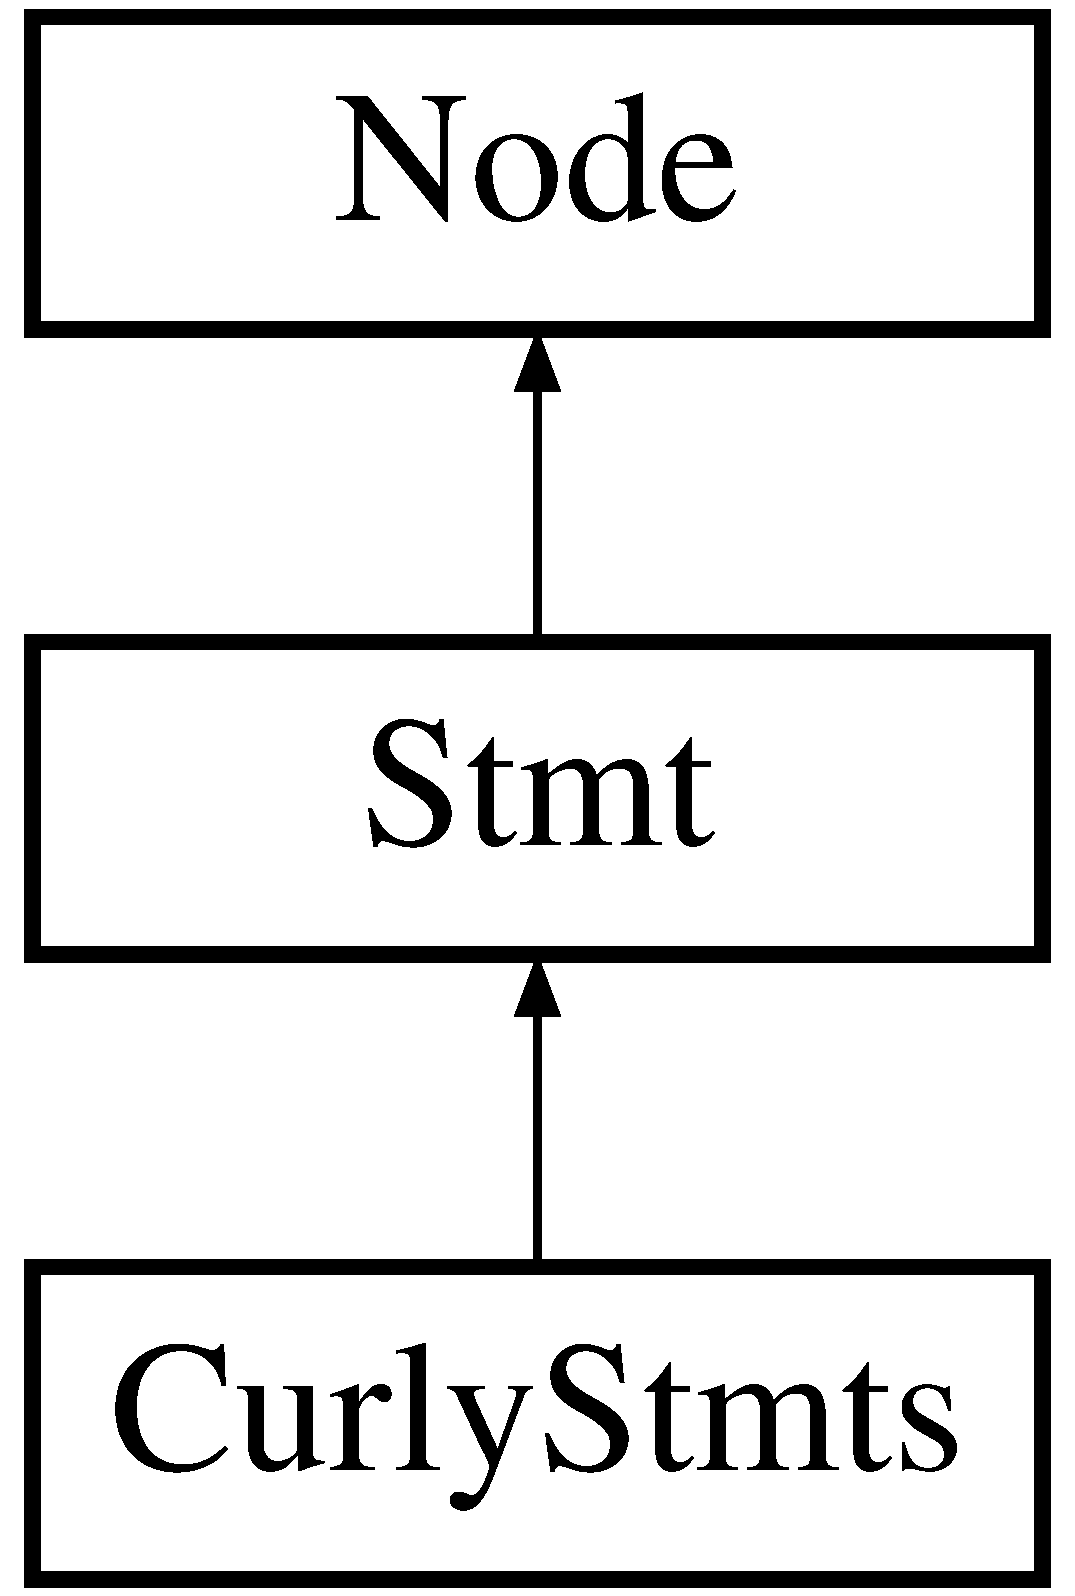
\includegraphics[height=3.000000cm]{classCurlyStmts}
\end{center}
\end{figure}
\subsection*{Public Member Functions}
\begin{DoxyCompactItemize}
\item 
\hypertarget{classCurlyStmts_a837fafafabe84db350f3c77b112f3ef4}{{\bfseries Curly\-Stmts} (\hyperlink{classStmts}{Stmts} $\ast$ss)}\label{classCurlyStmts_a837fafafabe84db350f3c77b112f3ef4}

\item 
\hypertarget{classCurlyStmts_af141e51f7aede8f95d094f9d91839666}{std\-::string \hyperlink{classCurlyStmts_af141e51f7aede8f95d094f9d91839666}{unparse} ()}\label{classCurlyStmts_af141e51f7aede8f95d094f9d91839666}

\begin{DoxyCompactList}\small\item\em Unparse the curly brackets and stmts (recursively) within. \end{DoxyCompactList}\end{DoxyCompactItemize}


\subsection{Detailed Description}
\hyperlink{classStmt}{Stmt} \-:\-:= '\{' \hyperlink{classStmts}{Stmts} '\}' This is for while loops ex\-: while (\hyperlink{classExpr}{Expr}) stmt -\/$>$ \{\hyperlink{classStmts}{Stmts}\}. 

The documentation for this class was generated from the following file\-:\begin{DoxyCompactItemize}
\item 
A\-S\-T.\-h\end{DoxyCompactItemize}

\hypertarget{classDashToken}{\section{Dash\-Token Class Reference}
\label{classDashToken}\index{Dash\-Token@{Dash\-Token}}
}
Inheritance diagram for Dash\-Token\-:\begin{figure}[H]
\begin{center}
\leavevmode
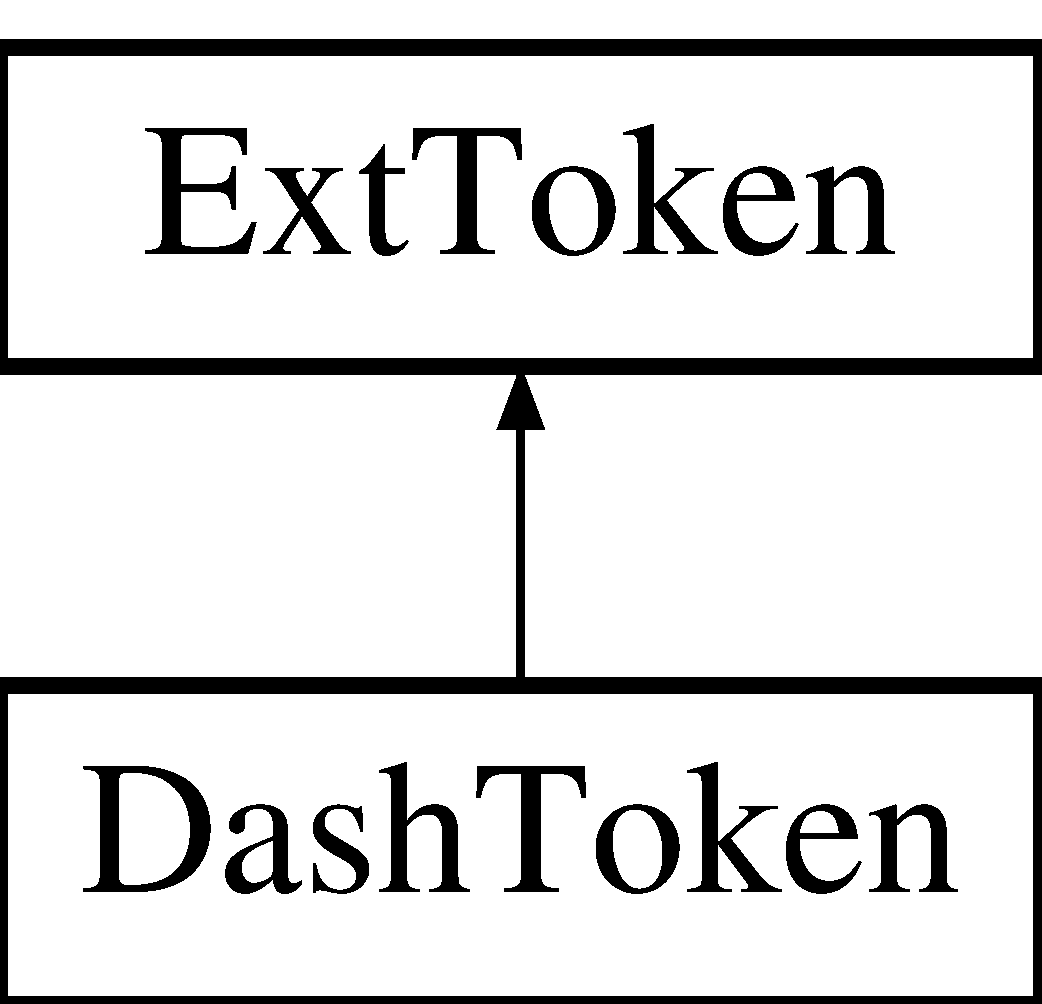
\includegraphics[height=2.000000cm]{classDashToken}
\end{center}
\end{figure}
\subsection*{Public Member Functions}
\begin{DoxyCompactItemize}
\item 
\hypertarget{classDashToken_a9570d66563405c728e679b63a44e53e2}{{\bfseries Dash\-Token} (\hyperlink{classParser}{Parser} $\ast$p, \hyperlink{classToken}{Token} $\ast$t)}\label{classDashToken_a9570d66563405c728e679b63a44e53e2}

\item 
\hypertarget{classDashToken_a703ca6afcd05ac4688c66b82e177bdbc}{\hyperlink{classParseResult}{Parse\-Result} {\bfseries led} (\hyperlink{classParseResult}{Parse\-Result} left)}\label{classDashToken_a703ca6afcd05ac4688c66b82e177bdbc}

\item 
\hypertarget{classDashToken_a02d79abb30dcab20081edb8e969885d2}{std\-::string {\bfseries description} ()}\label{classDashToken_a02d79abb30dcab20081edb8e969885d2}

\item 
\hypertarget{classDashToken_a1cf877584a85c06e884a182744e92b39}{int {\bfseries lbp} ()}\label{classDashToken_a1cf877584a85c06e884a182744e92b39}

\end{DoxyCompactItemize}
\subsection*{Additional Inherited Members}


The documentation for this class was generated from the following file\-:\begin{DoxyCompactItemize}
\item 
ext\-Token.\-h\end{DoxyCompactItemize}

\hypertarget{classDecl}{\section{Decl Class Reference}
\label{classDecl}\index{Decl@{Decl}}
}
Inheritance diagram for Decl\-:\begin{figure}[H]
\begin{center}
\leavevmode
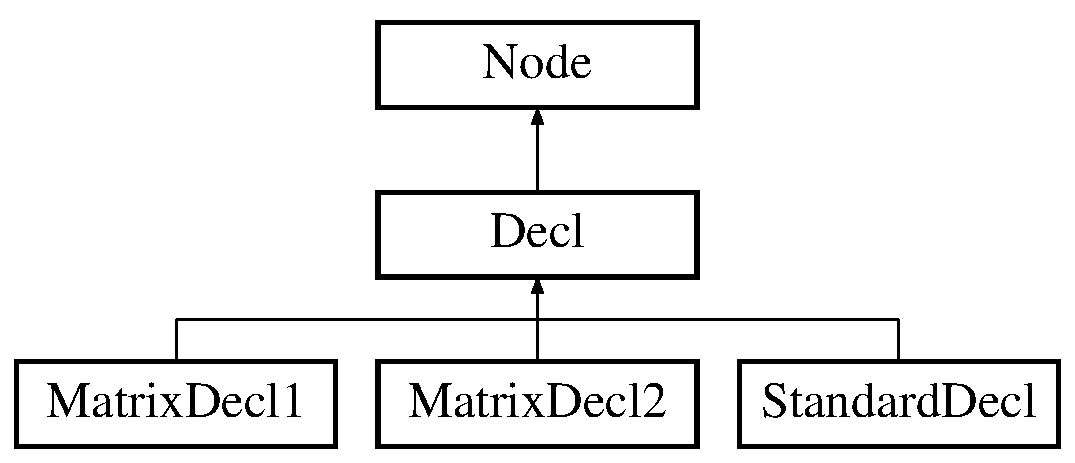
\includegraphics[height=3.000000cm]{classDecl}
\end{center}
\end{figure}
\subsection*{Additional Inherited Members}


The documentation for this class was generated from the following file\-:\begin{DoxyCompactItemize}
\item 
A\-S\-T.\-h\end{DoxyCompactItemize}

\hypertarget{classEmptyStmts}{\section{Empty\-Stmts Class Reference}
\label{classEmptyStmts}\index{Empty\-Stmts@{Empty\-Stmts}}
}


{\ttfamily \#include $<$A\-S\-T.\-h$>$}

Inheritance diagram for Empty\-Stmts\-:\begin{figure}[H]
\begin{center}
\leavevmode
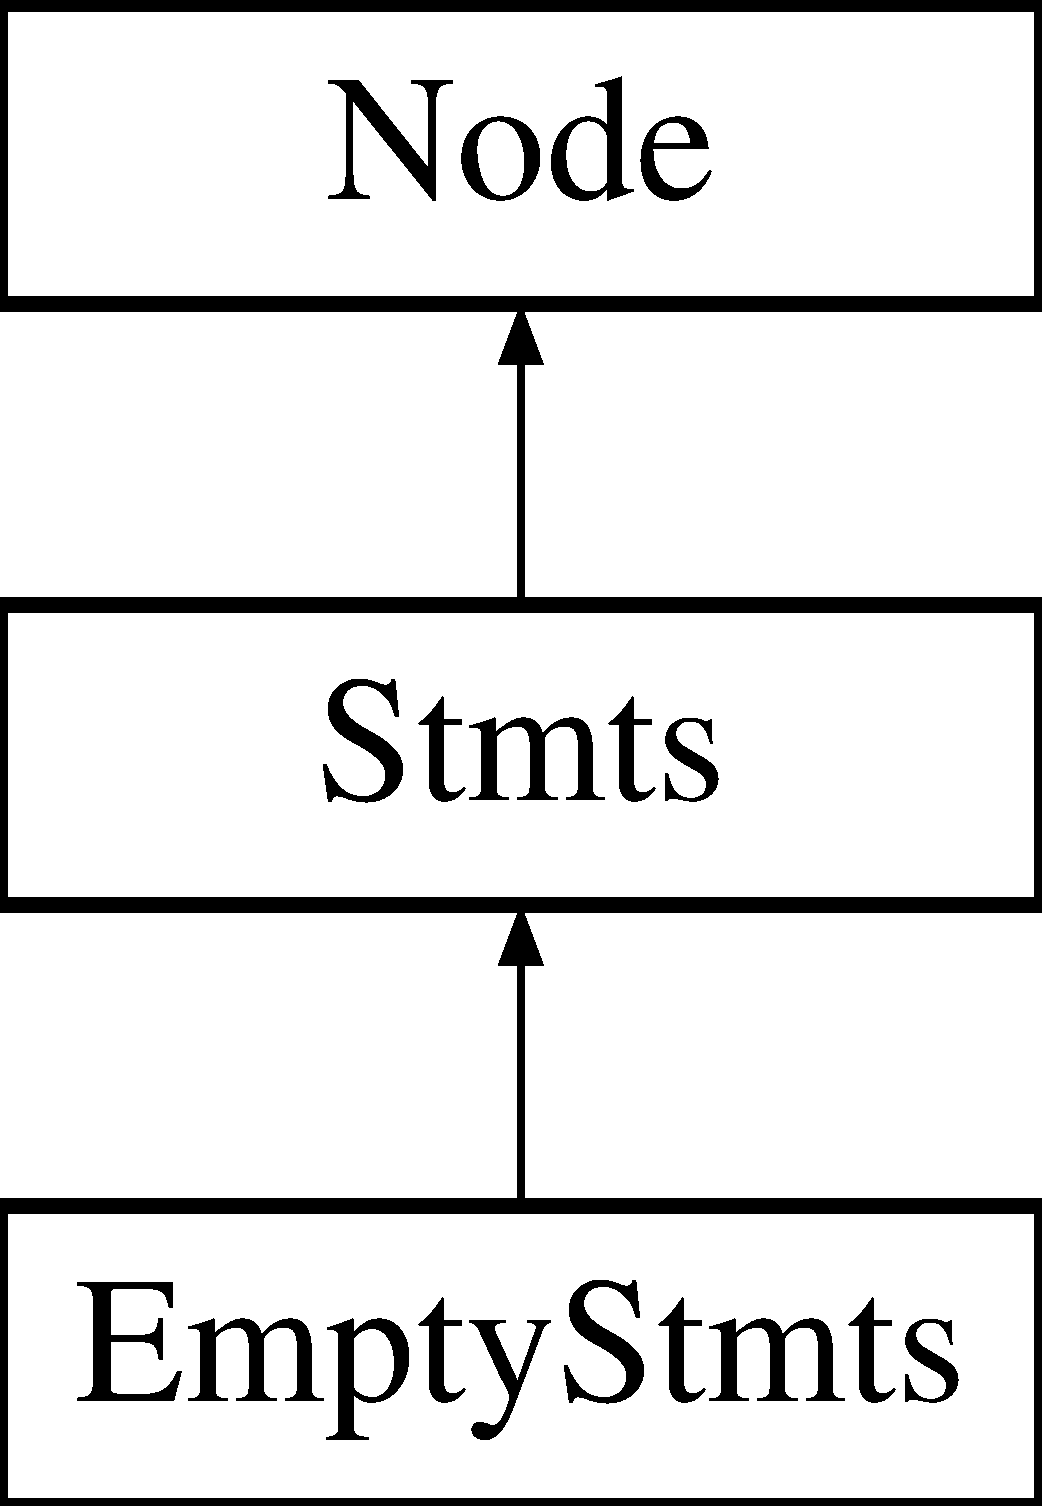
\includegraphics[height=3.000000cm]{classEmptyStmts}
\end{center}
\end{figure}
\subsection*{Public Member Functions}
\begin{DoxyCompactItemize}
\item 
\hypertarget{classEmptyStmts_a127064ef5c59227fc8452b31c65eb905}{std\-::string \hyperlink{classEmptyStmts_a127064ef5c59227fc8452b31c65eb905}{unparse} ()}\label{classEmptyStmts_a127064ef5c59227fc8452b31c65eb905}

\begin{DoxyCompactList}\small\item\em Unparse an empty \hyperlink{classStmts}{Stmts} (grammar line 2) \end{DoxyCompactList}\end{DoxyCompactItemize}


\subsection{Detailed Description}
\hyperlink{classStmts}{Stmts} \-:\-:= nothing to match 

The documentation for this class was generated from the following file\-:\begin{DoxyCompactItemize}
\item 
A\-S\-T.\-h\end{DoxyCompactItemize}

\hypertarget{classEndOfFileToken}{\section{End\-Of\-File\-Token Class Reference}
\label{classEndOfFileToken}\index{End\-Of\-File\-Token@{End\-Of\-File\-Token}}
}
Inheritance diagram for End\-Of\-File\-Token\-:\begin{figure}[H]
\begin{center}
\leavevmode
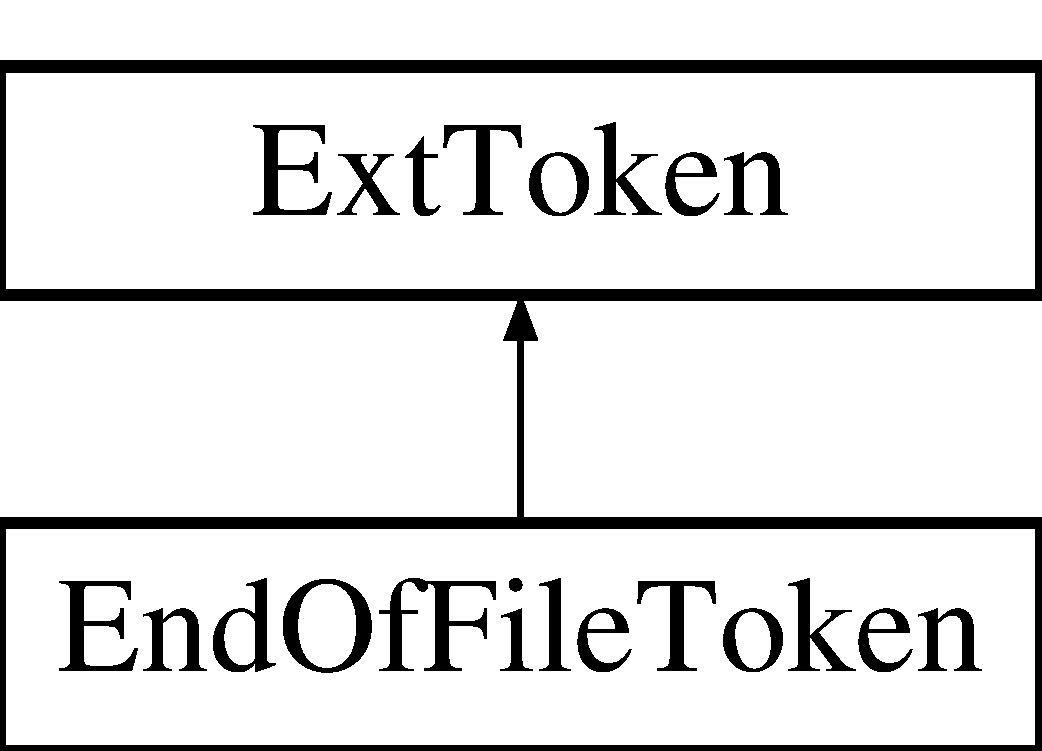
\includegraphics[height=2.000000cm]{classEndOfFileToken}
\end{center}
\end{figure}
\subsection*{Public Member Functions}
\begin{DoxyCompactItemize}
\item 
\hypertarget{classEndOfFileToken_a5c093bc13648a4f4df525ea4242e59d9}{{\bfseries End\-Of\-File\-Token} (\hyperlink{classParser}{Parser} $\ast$p, \hyperlink{classToken}{Token} $\ast$t)}\label{classEndOfFileToken_a5c093bc13648a4f4df525ea4242e59d9}

\item 
\hypertarget{classEndOfFileToken_a918312b101ca8cc7fb5ba4e56bc12b58}{std\-::string {\bfseries description} ()}\label{classEndOfFileToken_a918312b101ca8cc7fb5ba4e56bc12b58}

\end{DoxyCompactItemize}
\subsection*{Additional Inherited Members}


The documentation for this class was generated from the following file\-:\begin{DoxyCompactItemize}
\item 
ext\-Token.\-h\end{DoxyCompactItemize}

\hypertarget{classExpr}{\section{Expr Class Reference}
\label{classExpr}\index{Expr@{Expr}}
}
Inheritance diagram for Expr\-:\begin{figure}[H]
\begin{center}
\leavevmode
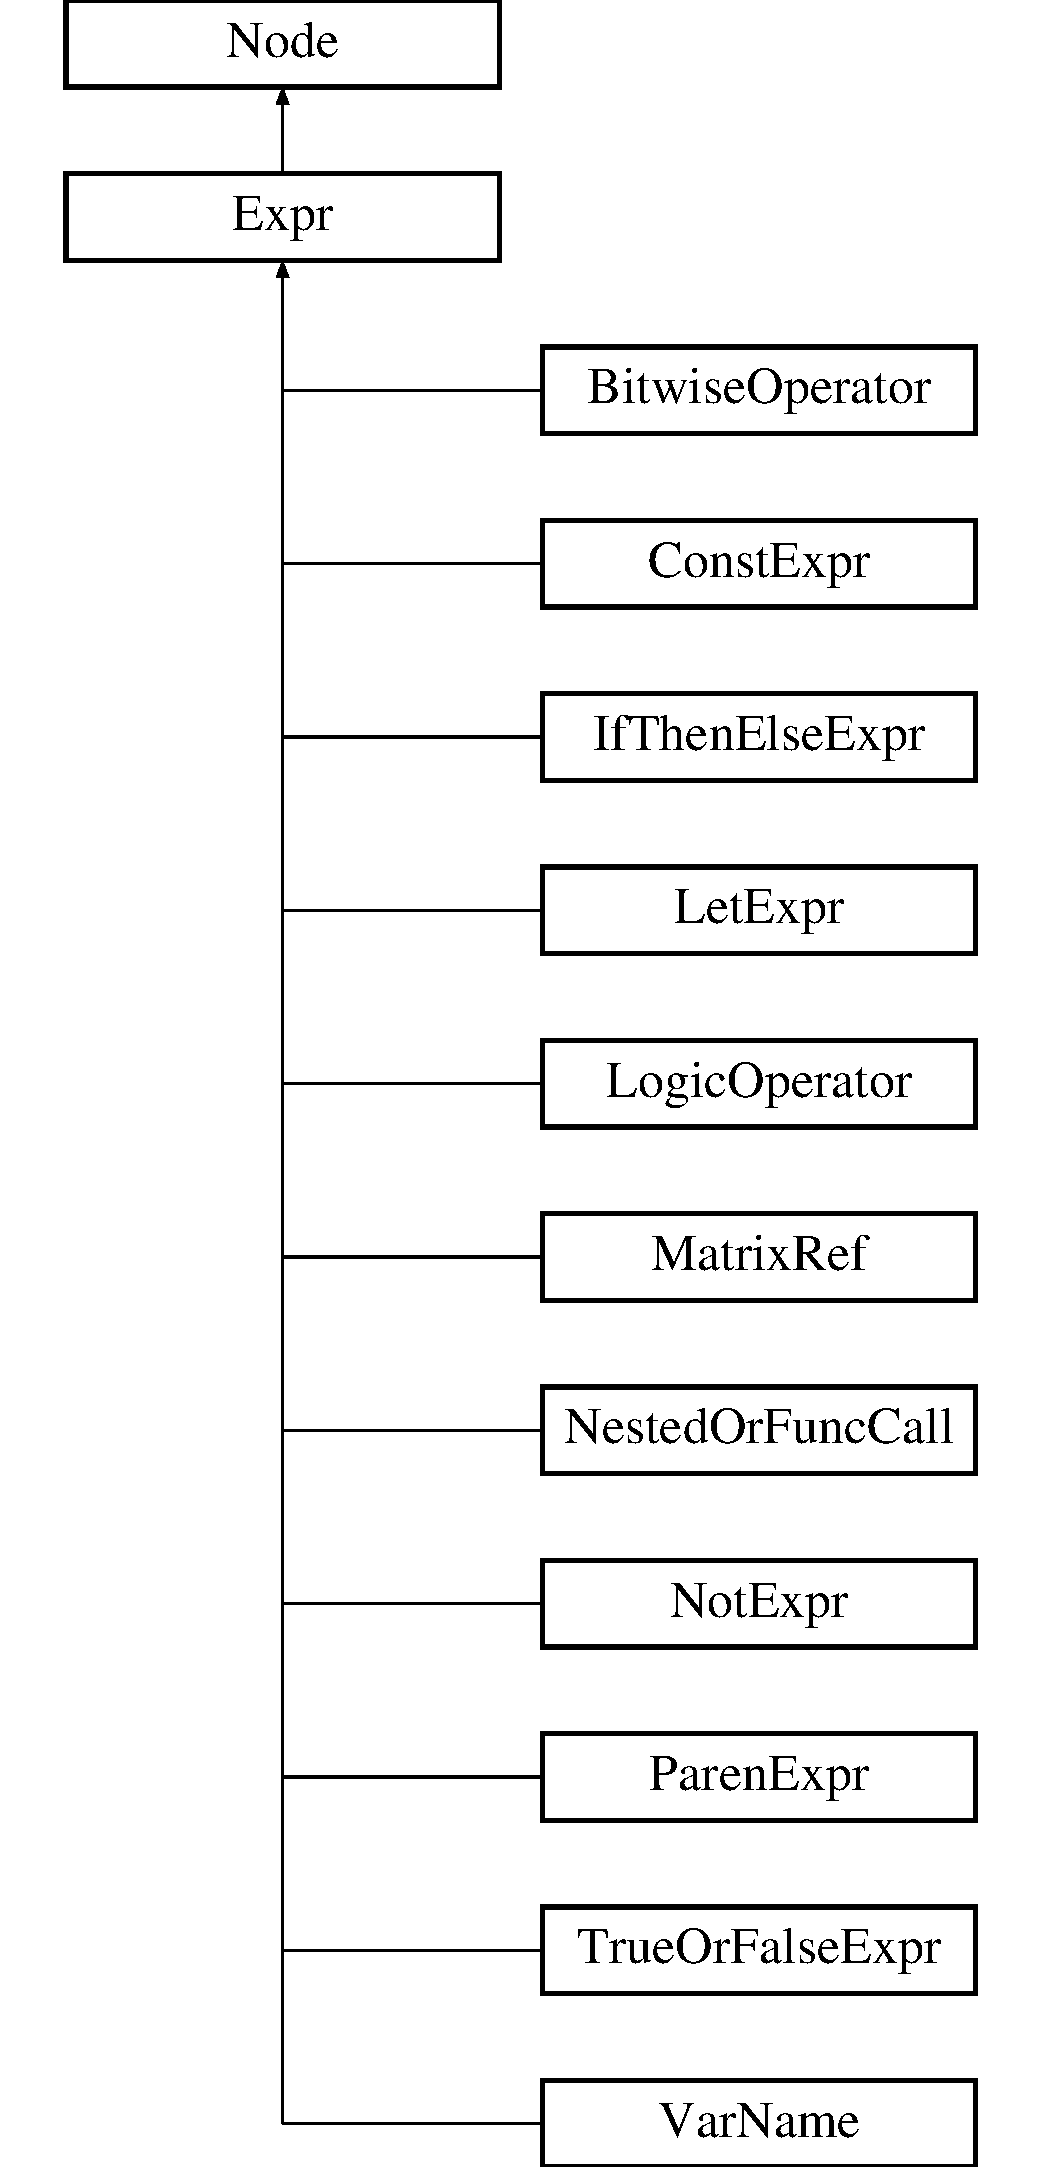
\includegraphics[height=12.000000cm]{classExpr}
\end{center}
\end{figure}
\subsection*{Additional Inherited Members}


The documentation for this class was generated from the following file\-:\begin{DoxyCompactItemize}
\item 
A\-S\-T.\-h\end{DoxyCompactItemize}

\hypertarget{classExtToken}{\section{Ext\-Token Class Reference}
\label{classExtToken}\index{Ext\-Token@{Ext\-Token}}
}
Inheritance diagram for Ext\-Token\-:\begin{figure}[H]
\begin{center}
\leavevmode
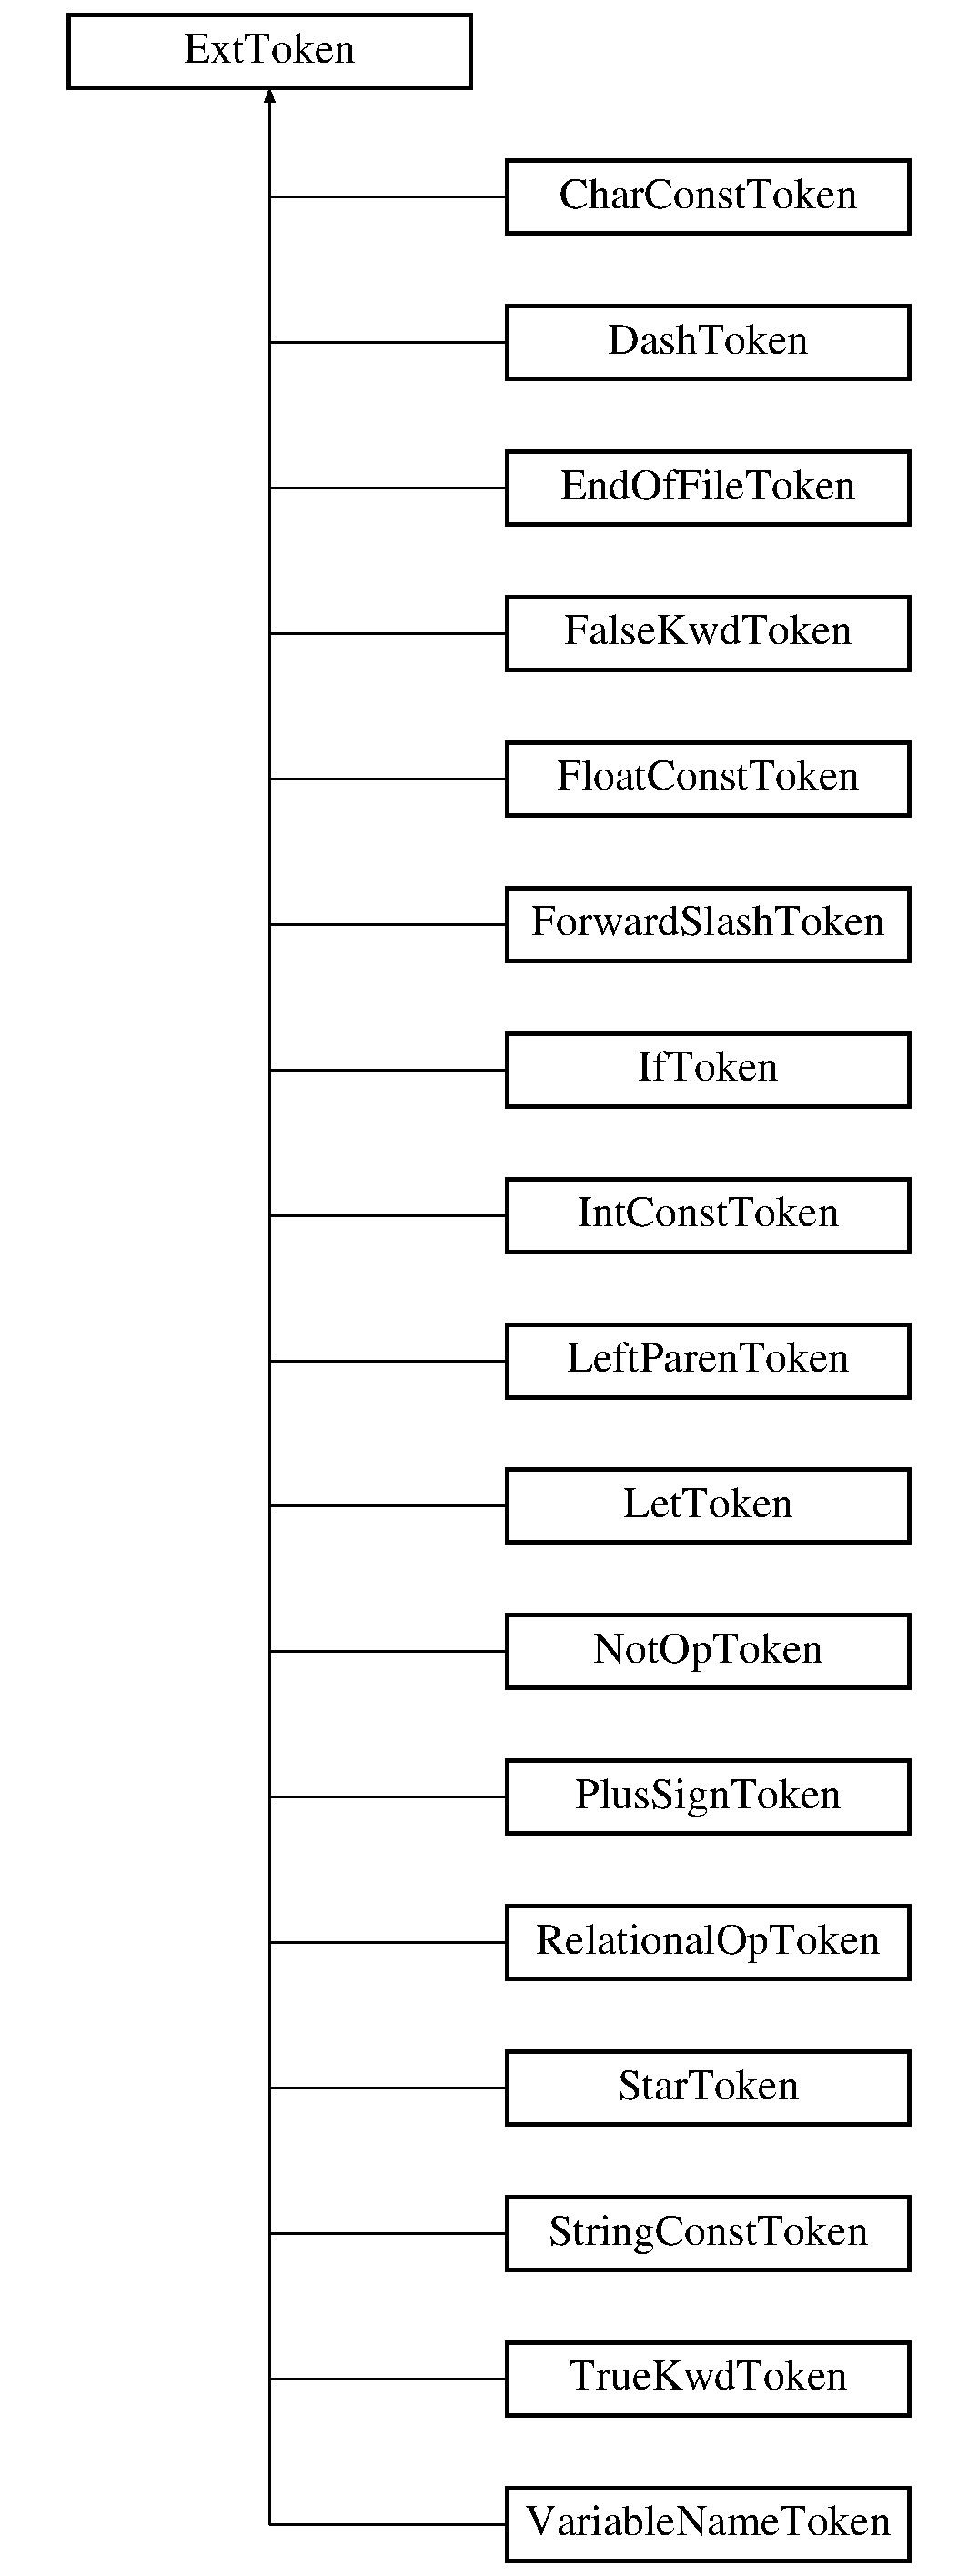
\includegraphics[height=12.000000cm]{classExtToken}
\end{center}
\end{figure}
\subsection*{Public Member Functions}
\begin{DoxyCompactItemize}
\item 
\hypertarget{classExtToken_a45a27528f391faf5679b7b30563ce846}{{\bfseries Ext\-Token} (\hyperlink{classParser}{Parser} $\ast$p, \hyperlink{classToken}{Token} $\ast$t)}\label{classExtToken_a45a27528f391faf5679b7b30563ce846}

\item 
\hypertarget{classExtToken_afa8972152abec42cd52b6f6f70a9a179}{{\bfseries Ext\-Token} (\hyperlink{classParser}{Parser} $\ast$p, \hyperlink{classToken}{Token} $\ast$t, std\-::string d)}\label{classExtToken_afa8972152abec42cd52b6f6f70a9a179}

\item 
\hypertarget{classExtToken_a5c21a5ffe91f212085259126652ab77c}{virtual \hyperlink{classParseResult}{Parse\-Result} {\bfseries nud} ()}\label{classExtToken_a5c21a5ffe91f212085259126652ab77c}

\item 
\hypertarget{classExtToken_afb2c9b0040e198d1d8aa2e041c5a7211}{virtual \hyperlink{classParseResult}{Parse\-Result} {\bfseries led} (\hyperlink{classParseResult}{Parse\-Result} left)}\label{classExtToken_afb2c9b0040e198d1d8aa2e041c5a7211}

\item 
\hypertarget{classExtToken_a6c0d61faa058b71147dd54bacee1db94}{virtual int {\bfseries lbp} ()}\label{classExtToken_a6c0d61faa058b71147dd54bacee1db94}

\item 
\hypertarget{classExtToken_a4ab6e72ac23235650b1756f794172ebb}{virtual std\-::string {\bfseries description} ()}\label{classExtToken_a4ab6e72ac23235650b1756f794172ebb}

\end{DoxyCompactItemize}
\subsection*{Public Attributes}
\begin{DoxyCompactItemize}
\item 
\hypertarget{classExtToken_a5af1643a542ef7ee8ca0f82706383ae3}{std\-::string {\bfseries lexeme}}\label{classExtToken_a5af1643a542ef7ee8ca0f82706383ae3}

\item 
\hypertarget{classExtToken_abbdaef42b65403cdc0247839ef95c875}{token\-Type {\bfseries terminal}}\label{classExtToken_abbdaef42b65403cdc0247839ef95c875}

\item 
\hypertarget{classExtToken_aa02995a897183b2a6ef758e541534e46}{\hyperlink{classExtToken}{Ext\-Token} $\ast$ {\bfseries next}}\label{classExtToken_aa02995a897183b2a6ef758e541534e46}

\item 
\hypertarget{classExtToken_af70d22156d5f8e855a8b0d92a82706ba}{\hyperlink{classParser}{Parser} $\ast$ {\bfseries parser}}\label{classExtToken_af70d22156d5f8e855a8b0d92a82706ba}

\end{DoxyCompactItemize}


The documentation for this class was generated from the following file\-:\begin{DoxyCompactItemize}
\item 
ext\-Token.\-h\end{DoxyCompactItemize}

\hypertarget{classFalseKwdToken}{\section{False\-Kwd\-Token Class Reference}
\label{classFalseKwdToken}\index{False\-Kwd\-Token@{False\-Kwd\-Token}}
}
Inheritance diagram for False\-Kwd\-Token\-:\begin{figure}[H]
\begin{center}
\leavevmode
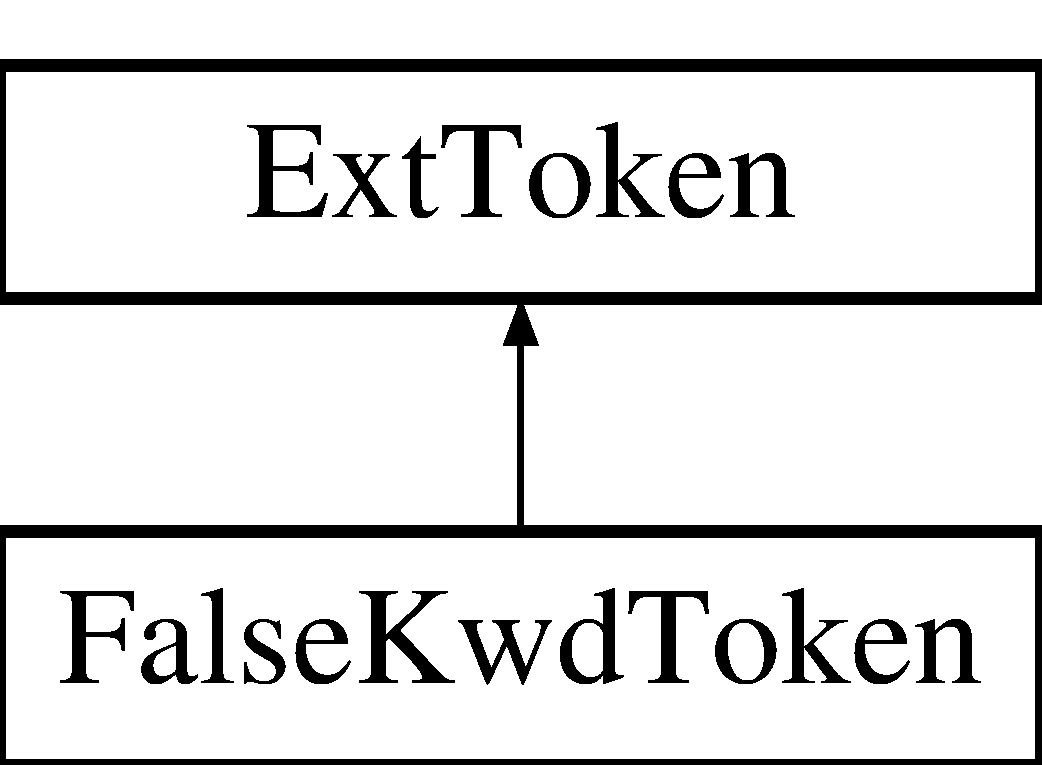
\includegraphics[height=2.000000cm]{classFalseKwdToken}
\end{center}
\end{figure}
\subsection*{Public Member Functions}
\begin{DoxyCompactItemize}
\item 
\hypertarget{classFalseKwdToken_add6402d29fd7b22253a0dc73370597e4}{{\bfseries False\-Kwd\-Token} (\hyperlink{classParser}{Parser} $\ast$p, \hyperlink{classToken}{Token} $\ast$t)}\label{classFalseKwdToken_add6402d29fd7b22253a0dc73370597e4}

\item 
\hypertarget{classFalseKwdToken_adc06b0433535d552c1e7f8076d756fb3}{\hyperlink{classParseResult}{Parse\-Result} {\bfseries nud} ()}\label{classFalseKwdToken_adc06b0433535d552c1e7f8076d756fb3}

\item 
\hypertarget{classFalseKwdToken_a8351fad7090214687138e113b5a581f1}{std\-::string {\bfseries description} ()}\label{classFalseKwdToken_a8351fad7090214687138e113b5a581f1}

\end{DoxyCompactItemize}
\subsection*{Additional Inherited Members}


The documentation for this class was generated from the following file\-:\begin{DoxyCompactItemize}
\item 
ext\-Token.\-h\end{DoxyCompactItemize}

\hypertarget{classFloatConstToken}{\section{Float\-Const\-Token Class Reference}
\label{classFloatConstToken}\index{Float\-Const\-Token@{Float\-Const\-Token}}
}
Inheritance diagram for Float\-Const\-Token\-:\begin{figure}[H]
\begin{center}
\leavevmode
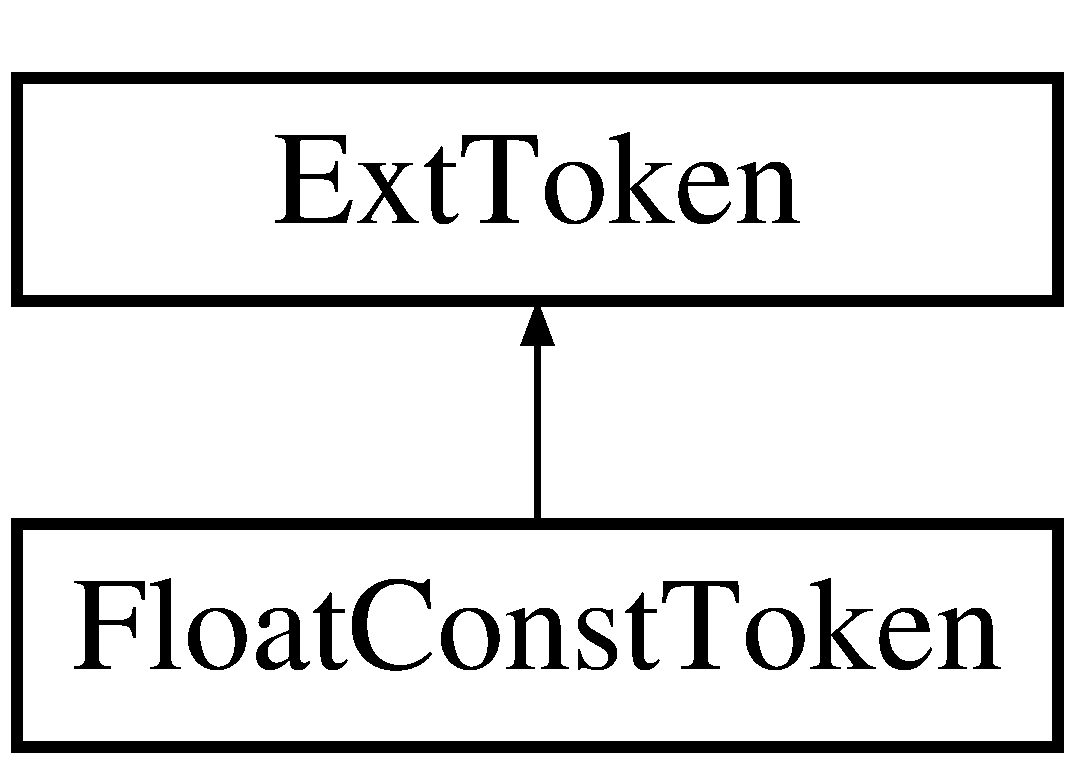
\includegraphics[height=2.000000cm]{classFloatConstToken}
\end{center}
\end{figure}
\subsection*{Public Member Functions}
\begin{DoxyCompactItemize}
\item 
\hypertarget{classFloatConstToken_aecee1d0e4e8a9410701c68c30858a4db}{{\bfseries Float\-Const\-Token} (\hyperlink{classParser}{Parser} $\ast$p, \hyperlink{classToken}{Token} $\ast$t)}\label{classFloatConstToken_aecee1d0e4e8a9410701c68c30858a4db}

\item 
\hypertarget{classFloatConstToken_a991e92ae34d0b01a3b1dd08ed01b8e6e}{\hyperlink{classParseResult}{Parse\-Result} {\bfseries nud} ()}\label{classFloatConstToken_a991e92ae34d0b01a3b1dd08ed01b8e6e}

\item 
\hypertarget{classFloatConstToken_a529b6d3ad479b0f6b940a82ba48b98c0}{std\-::string {\bfseries description} ()}\label{classFloatConstToken_a529b6d3ad479b0f6b940a82ba48b98c0}

\end{DoxyCompactItemize}
\subsection*{Additional Inherited Members}


The documentation for this class was generated from the following file\-:\begin{DoxyCompactItemize}
\item 
ext\-Token.\-h\end{DoxyCompactItemize}

\hypertarget{classForwardSlashToken}{\section{Forward\-Slash\-Token Class Reference}
\label{classForwardSlashToken}\index{Forward\-Slash\-Token@{Forward\-Slash\-Token}}
}
Inheritance diagram for Forward\-Slash\-Token\-:\begin{figure}[H]
\begin{center}
\leavevmode
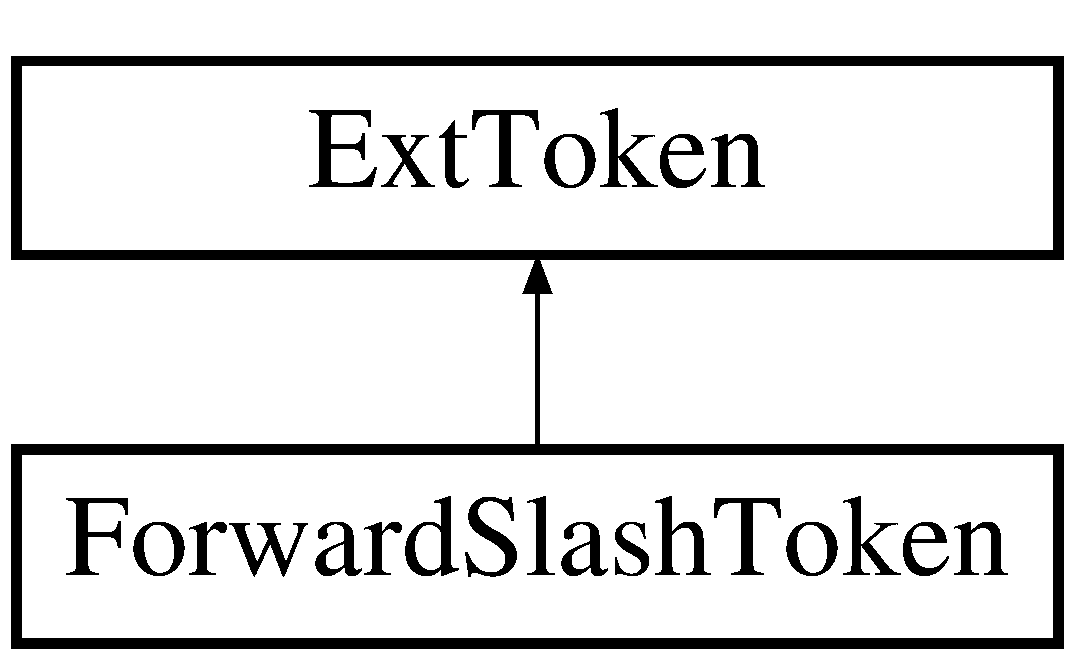
\includegraphics[height=2.000000cm]{classForwardSlashToken}
\end{center}
\end{figure}
\subsection*{Public Member Functions}
\begin{DoxyCompactItemize}
\item 
\hypertarget{classForwardSlashToken_ae818840269cd15f6f6b00929fb4eb979}{{\bfseries Forward\-Slash\-Token} (\hyperlink{classParser}{Parser} $\ast$p, \hyperlink{classToken}{Token} $\ast$t)}\label{classForwardSlashToken_ae818840269cd15f6f6b00929fb4eb979}

\item 
\hypertarget{classForwardSlashToken_ac2dda7b791ab555e4323f17baaf323e1}{\hyperlink{classParseResult}{Parse\-Result} {\bfseries led} (\hyperlink{classParseResult}{Parse\-Result} left)}\label{classForwardSlashToken_ac2dda7b791ab555e4323f17baaf323e1}

\item 
\hypertarget{classForwardSlashToken_ac27b1ab175ec08c468bd0d4c41636a5c}{std\-::string {\bfseries description} ()}\label{classForwardSlashToken_ac27b1ab175ec08c468bd0d4c41636a5c}

\item 
\hypertarget{classForwardSlashToken_ad65829044355922a291dfbfd3052b183}{int {\bfseries lbp} ()}\label{classForwardSlashToken_ad65829044355922a291dfbfd3052b183}

\end{DoxyCompactItemize}
\subsection*{Additional Inherited Members}


The documentation for this class was generated from the following file\-:\begin{DoxyCompactItemize}
\item 
ext\-Token.\-h\end{DoxyCompactItemize}

\hypertarget{classIfElseStmt}{\section{If\-Else\-Stmt Class Reference}
\label{classIfElseStmt}\index{If\-Else\-Stmt@{If\-Else\-Stmt}}
}


\hyperlink{classStmt}{Stmt} \-:\-:= 'if' '(' \hyperlink{classExpr}{Expr} ')' \hyperlink{classStmt}{Stmt} 'else' \hyperlink{classStmt}{Stmt}.  




{\ttfamily \#include $<$A\-S\-T.\-h$>$}

Inheritance diagram for If\-Else\-Stmt\-:\begin{figure}[H]
\begin{center}
\leavevmode
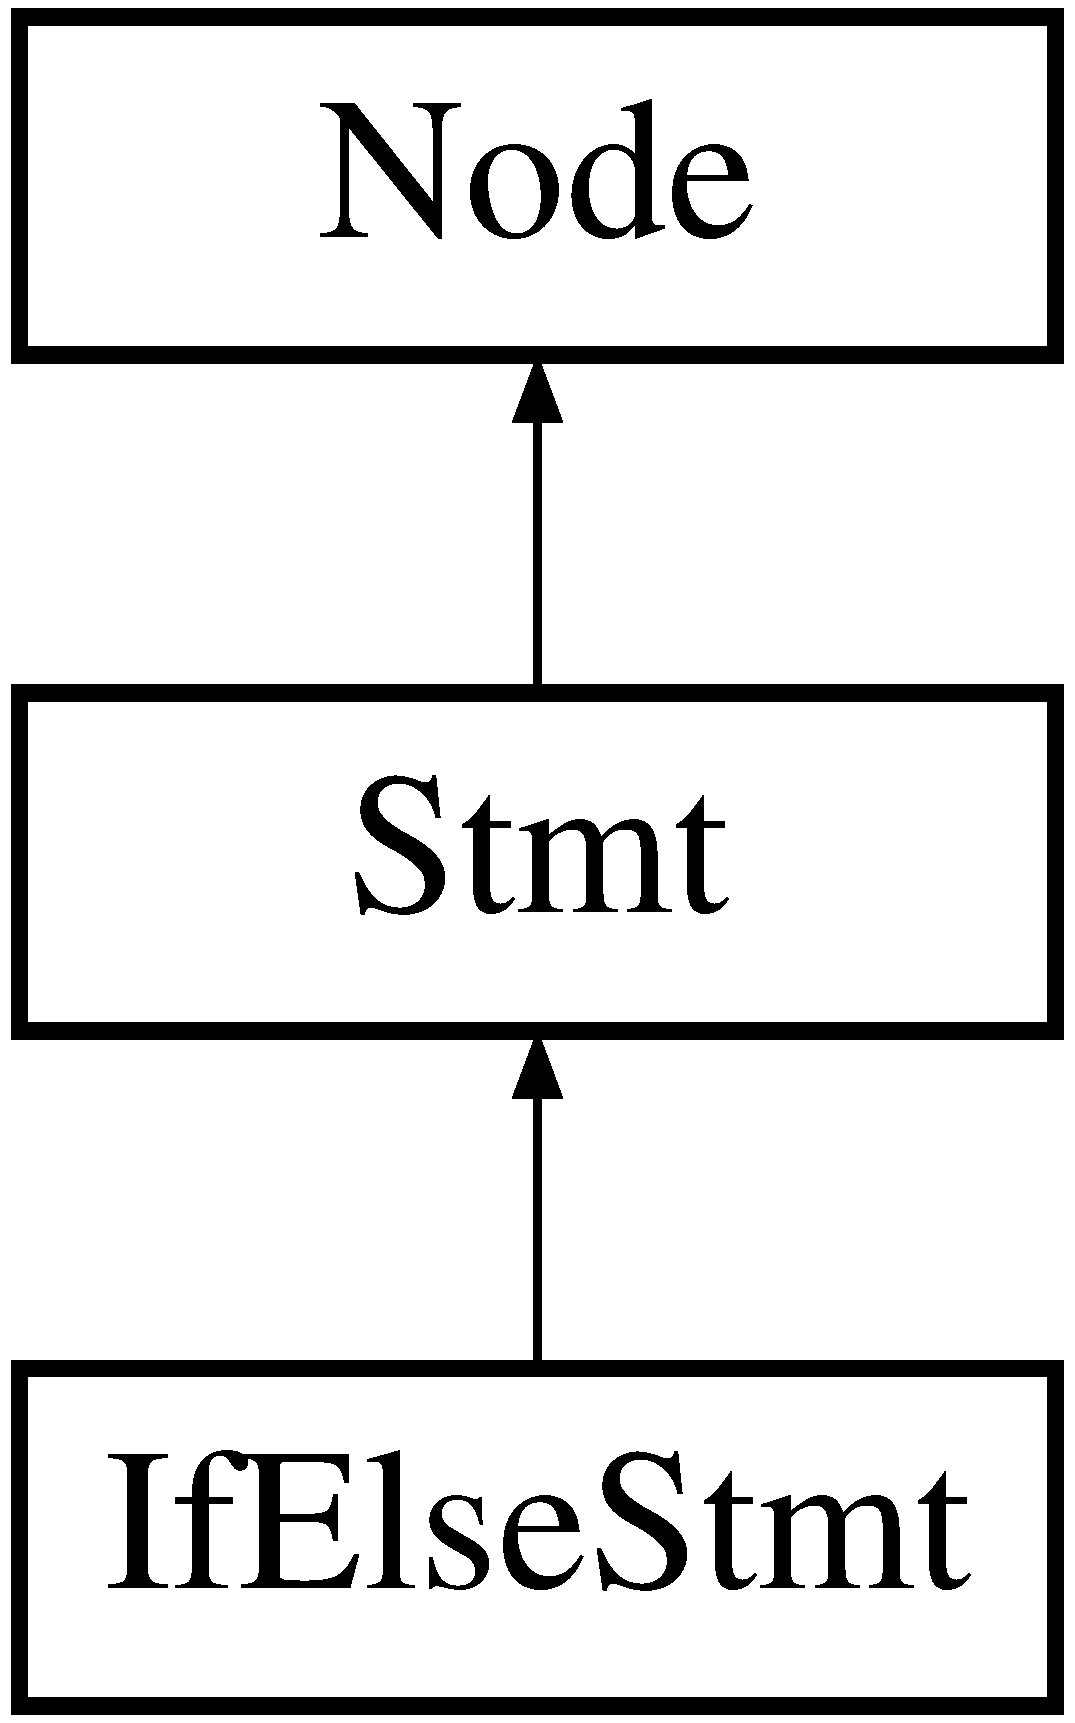
\includegraphics[height=3.000000cm]{classIfElseStmt}
\end{center}
\end{figure}
\subsection*{Public Member Functions}
\begin{DoxyCompactItemize}
\item 
\hypertarget{classIfElseStmt_a9e0fde33a0889aa64175dfdf7e7326da}{{\bfseries If\-Else\-Stmt} (\hyperlink{classExpr}{Expr} $\ast$e, \hyperlink{classStmt}{Stmt} $\ast$s1, \hyperlink{classStmt}{Stmt} $\ast$s2)}\label{classIfElseStmt_a9e0fde33a0889aa64175dfdf7e7326da}

\item 
\hypertarget{classIfElseStmt_a82267559f8fdd5f10cf14e616f3867f2}{std\-::string \hyperlink{classIfElseStmt_a82267559f8fdd5f10cf14e616f3867f2}{unparse} ()}\label{classIfElseStmt_a82267559f8fdd5f10cf14e616f3867f2}

\begin{DoxyCompactList}\small\item\em Unparse in proper 'if else' form as denoted in grammar. \end{DoxyCompactList}\end{DoxyCompactItemize}


\subsection{Detailed Description}
\hyperlink{classStmt}{Stmt} \-:\-:= 'if' '(' \hyperlink{classExpr}{Expr} ')' \hyperlink{classStmt}{Stmt} 'else' \hyperlink{classStmt}{Stmt}. 

The documentation for this class was generated from the following file\-:\begin{DoxyCompactItemize}
\item 
A\-S\-T.\-h\end{DoxyCompactItemize}

\hypertarget{classIfStmt}{\section{If\-Stmt Class Reference}
\label{classIfStmt}\index{If\-Stmt@{If\-Stmt}}
}


\hyperlink{classStmt}{Stmt}\-:\-:= 'if' '('\hyperlink{classExpr}{Expr}')' \hyperlink{classStmt}{Stmt}.  




{\ttfamily \#include $<$A\-S\-T.\-h$>$}

Inheritance diagram for If\-Stmt\-:\begin{figure}[H]
\begin{center}
\leavevmode
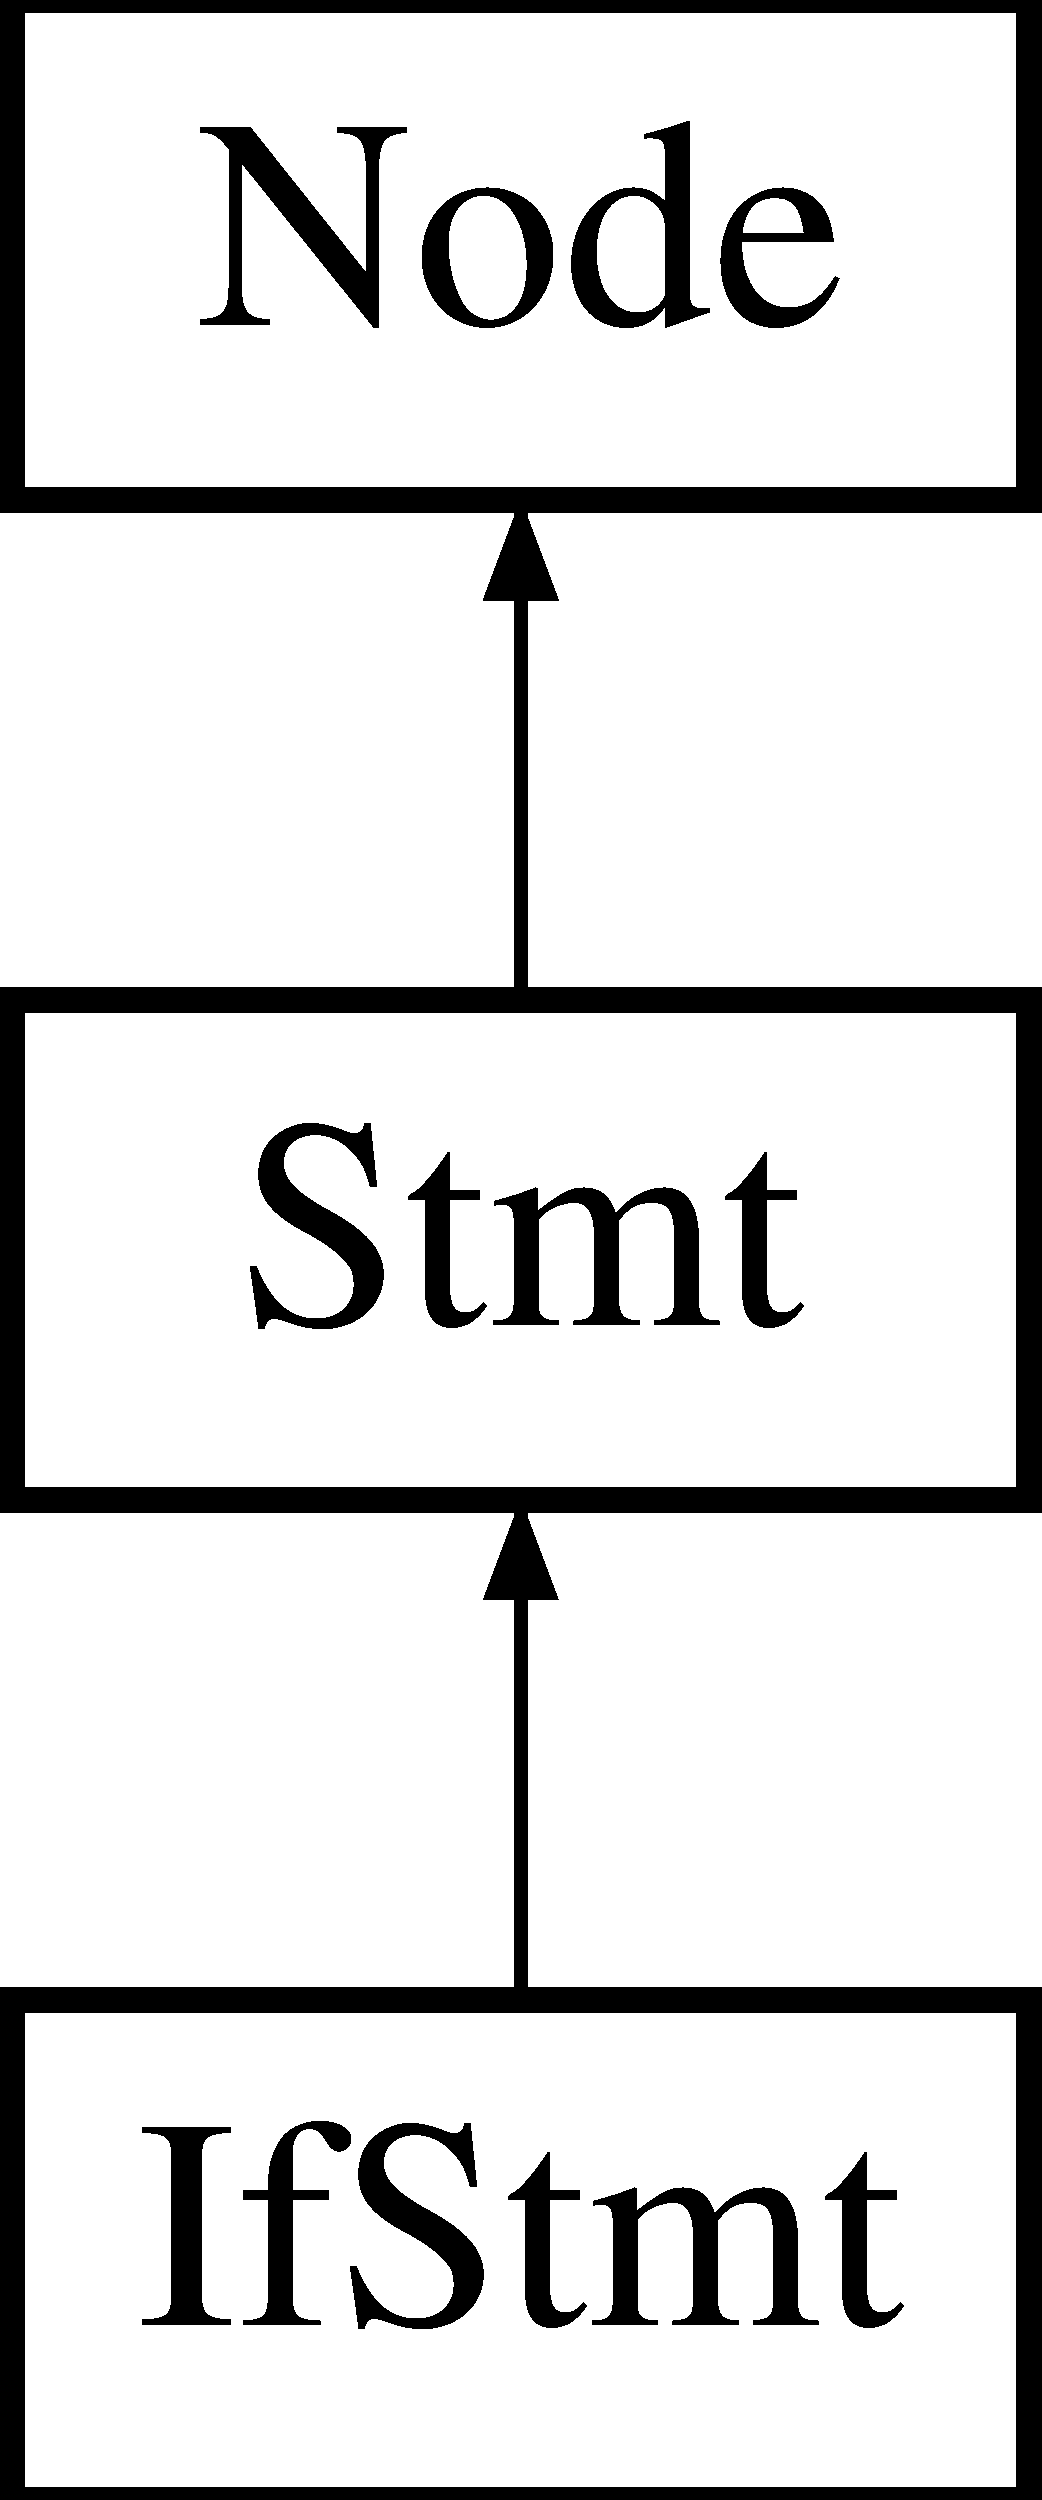
\includegraphics[height=3.000000cm]{classIfStmt}
\end{center}
\end{figure}
\subsection*{Public Member Functions}
\begin{DoxyCompactItemize}
\item 
\hypertarget{classIfStmt_a917206365fb4307ede6751d2d00e0a58}{{\bfseries If\-Stmt} (\hyperlink{classExpr}{Expr} $\ast$e, \hyperlink{classStmt}{Stmt} $\ast$s)}\label{classIfStmt_a917206365fb4307ede6751d2d00e0a58}

\item 
\hypertarget{classIfStmt_a615e8785edb068f24e19f3ce7863f2ce}{std\-::string \hyperlink{classIfStmt_a615e8785edb068f24e19f3ce7863f2ce}{unparse} ()}\label{classIfStmt_a615e8785edb068f24e19f3ce7863f2ce}

\begin{DoxyCompactList}\small\item\em Unparse in proper 'if' statement form as denoted in grammar. \end{DoxyCompactList}\end{DoxyCompactItemize}


\subsection{Detailed Description}
\hyperlink{classStmt}{Stmt}\-:\-:= 'if' '('\hyperlink{classExpr}{Expr}')' \hyperlink{classStmt}{Stmt}. 

The documentation for this class was generated from the following file\-:\begin{DoxyCompactItemize}
\item 
A\-S\-T.\-h\end{DoxyCompactItemize}

\hypertarget{classIfThenElseExpr}{\section{If\-Then\-Else\-Expr Class Reference}
\label{classIfThenElseExpr}\index{If\-Then\-Else\-Expr@{If\-Then\-Else\-Expr}}
}


\hyperlink{classExpr}{Expr} \-:\-:= 'if' \hyperlink{classExpr}{Expr} 'then' \hyperlink{classExpr}{Expr} 'else' \hyperlink{classExpr}{Expr} //\-If\-Expr.  




{\ttfamily \#include $<$A\-S\-T.\-h$>$}

Inheritance diagram for If\-Then\-Else\-Expr\-:\begin{figure}[H]
\begin{center}
\leavevmode
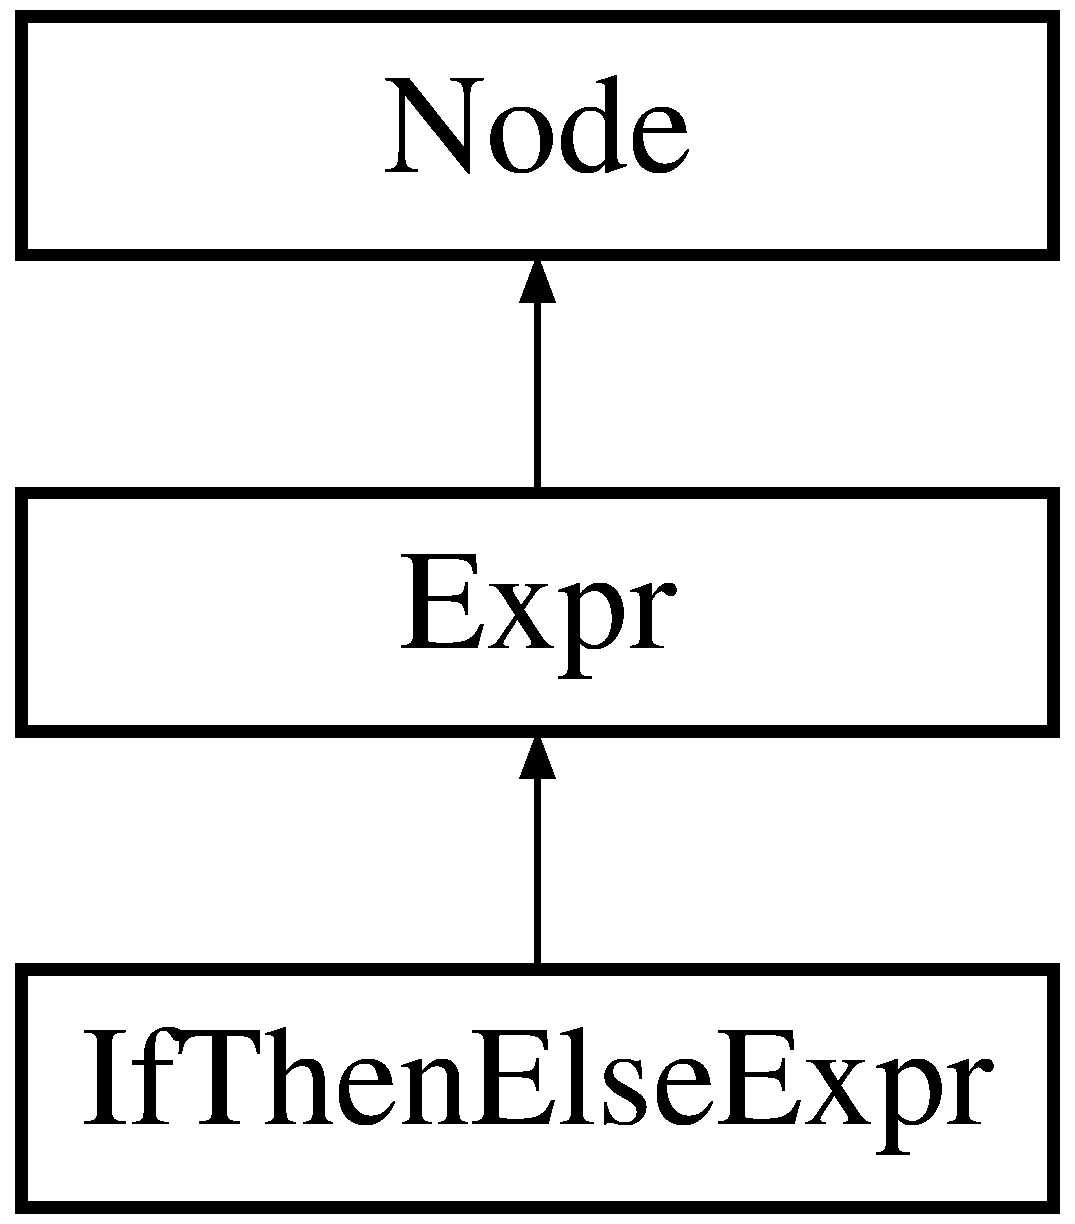
\includegraphics[height=3.000000cm]{classIfThenElseExpr}
\end{center}
\end{figure}
\subsection*{Public Member Functions}
\begin{DoxyCompactItemize}
\item 
\hypertarget{classIfThenElseExpr_a8e5fe13dd7707af3f549f5df53aa5dc3}{{\bfseries If\-Then\-Else\-Expr} (\hyperlink{classExpr}{Expr} $\ast$e1, \hyperlink{classExpr}{Expr} $\ast$e2, \hyperlink{classExpr}{Expr} $\ast$e3)}\label{classIfThenElseExpr_a8e5fe13dd7707af3f549f5df53aa5dc3}

\item 
\hypertarget{classIfThenElseExpr_a1686a9926fe0017d7cf8dd86c7ab79a0}{std\-::string \hyperlink{classIfThenElseExpr_a1686a9926fe0017d7cf8dd86c7ab79a0}{unparse} ()}\label{classIfThenElseExpr_a1686a9926fe0017d7cf8dd86c7ab79a0}

\begin{DoxyCompactList}\small\item\em Unparse in proper 'If Then Else' form as denoted in grammar. \end{DoxyCompactList}\end{DoxyCompactItemize}


\subsection{Detailed Description}
\hyperlink{classExpr}{Expr} \-:\-:= 'if' \hyperlink{classExpr}{Expr} 'then' \hyperlink{classExpr}{Expr} 'else' \hyperlink{classExpr}{Expr} //\-If\-Expr. 

The documentation for this class was generated from the following file\-:\begin{DoxyCompactItemize}
\item 
A\-S\-T.\-h\end{DoxyCompactItemize}

\hypertarget{classIfToken}{\section{If\-Token Class Reference}
\label{classIfToken}\index{If\-Token@{If\-Token}}
}
Inheritance diagram for If\-Token\-:\begin{figure}[H]
\begin{center}
\leavevmode
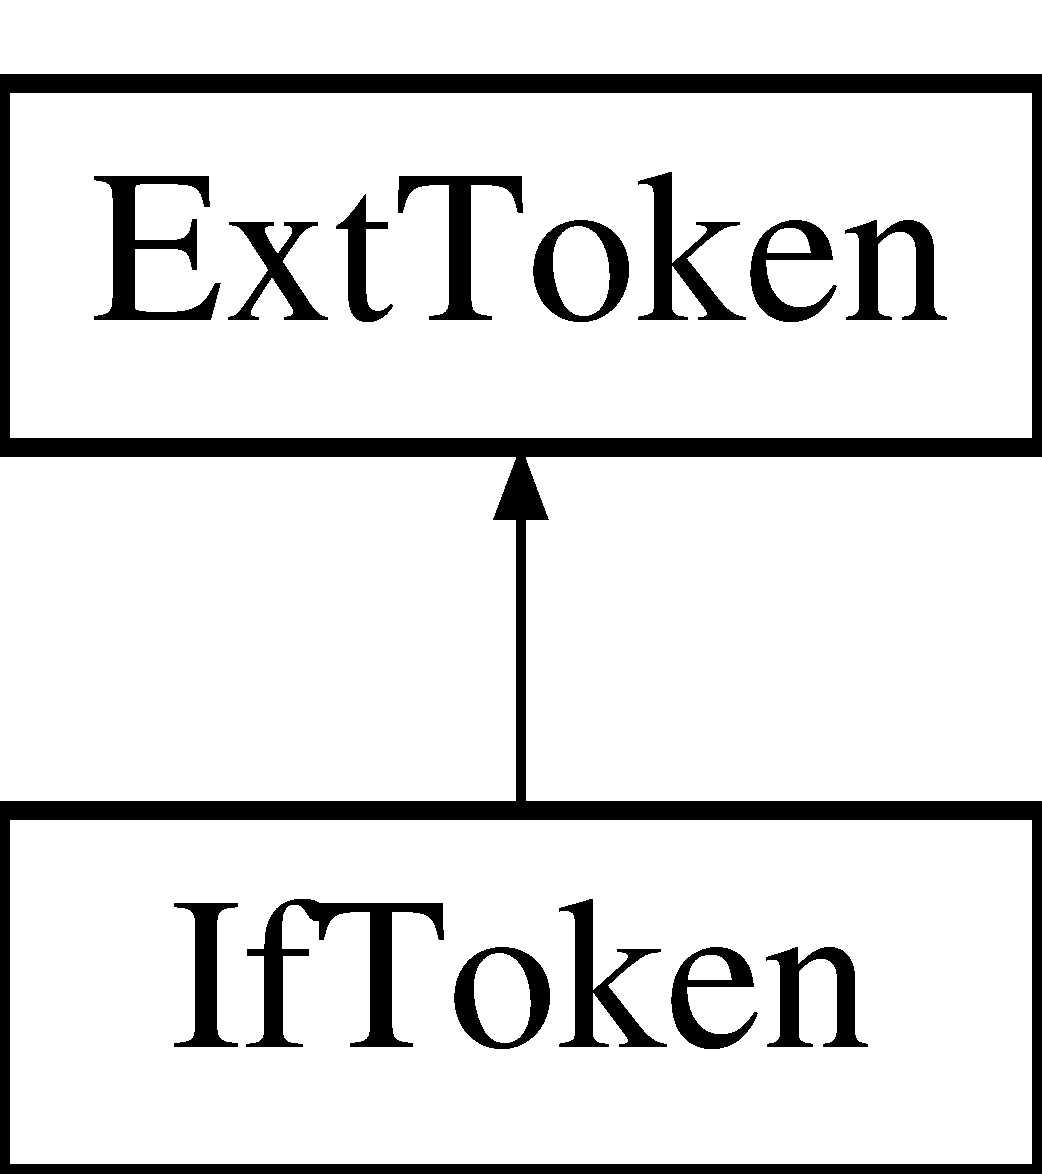
\includegraphics[height=2.000000cm]{classIfToken}
\end{center}
\end{figure}
\subsection*{Public Member Functions}
\begin{DoxyCompactItemize}
\item 
\hypertarget{classIfToken_a607028595b06b8a950000ba3e82329db}{{\bfseries If\-Token} (\hyperlink{classParser}{Parser} $\ast$p, \hyperlink{classToken}{Token} $\ast$t)}\label{classIfToken_a607028595b06b8a950000ba3e82329db}

\item 
\hypertarget{classIfToken_add06bd79ce755fd5503f78e507109e52}{\hyperlink{classParseResult}{Parse\-Result} {\bfseries nud} ()}\label{classIfToken_add06bd79ce755fd5503f78e507109e52}

\item 
\hypertarget{classIfToken_aad226162c5649920c13c2a9e9e7a3617}{std\-::string {\bfseries description} ()}\label{classIfToken_aad226162c5649920c13c2a9e9e7a3617}

\item 
\hypertarget{classIfToken_abfd39ff4c4818d382bf0b97fd097c478}{int {\bfseries lbp} ()}\label{classIfToken_abfd39ff4c4818d382bf0b97fd097c478}

\end{DoxyCompactItemize}
\subsection*{Additional Inherited Members}


The documentation for this class was generated from the following file\-:\begin{DoxyCompactItemize}
\item 
ext\-Token.\-h\end{DoxyCompactItemize}

\hypertarget{classIntConstToken}{\section{Int\-Const\-Token Class Reference}
\label{classIntConstToken}\index{Int\-Const\-Token@{Int\-Const\-Token}}
}
Inheritance diagram for Int\-Const\-Token\-:\begin{figure}[H]
\begin{center}
\leavevmode
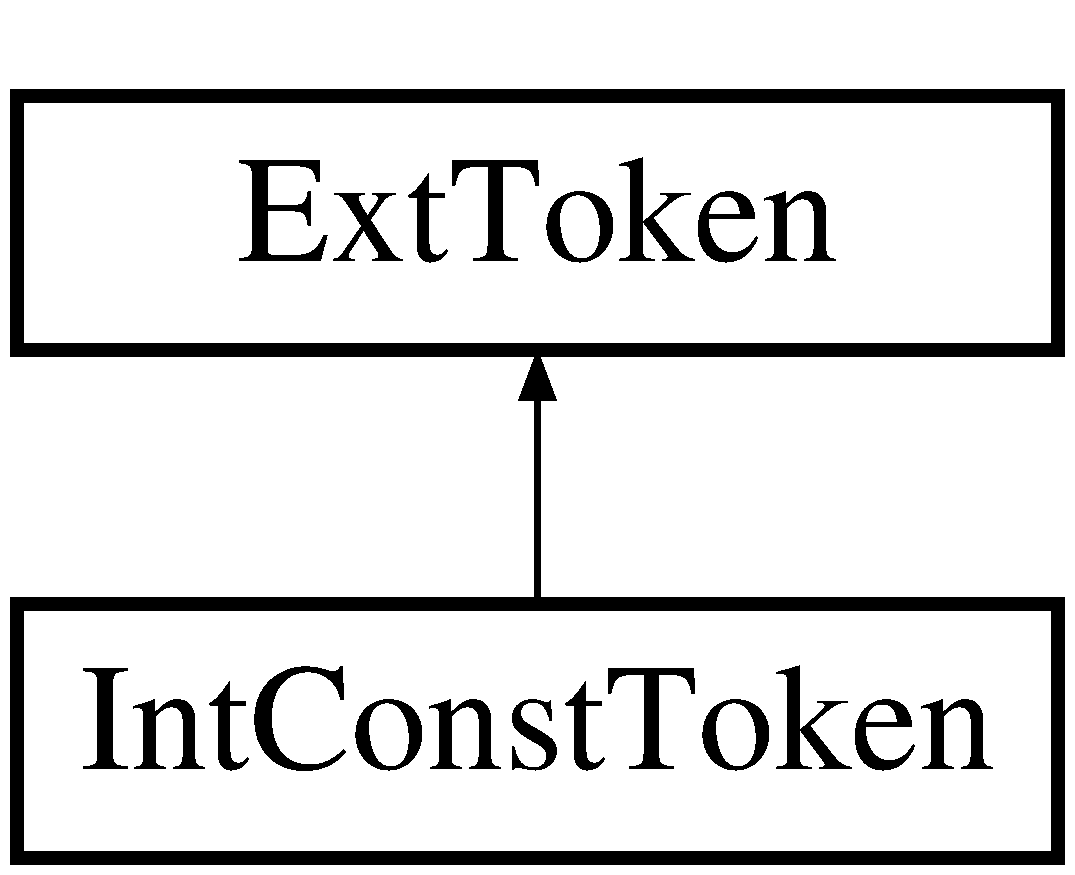
\includegraphics[height=2.000000cm]{classIntConstToken}
\end{center}
\end{figure}
\subsection*{Public Member Functions}
\begin{DoxyCompactItemize}
\item 
\hypertarget{classIntConstToken_a14c6bf0af5a915969b4fef1758067af3}{{\bfseries Int\-Const\-Token} (\hyperlink{classParser}{Parser} $\ast$p, \hyperlink{classToken}{Token} $\ast$t)}\label{classIntConstToken_a14c6bf0af5a915969b4fef1758067af3}

\item 
\hypertarget{classIntConstToken_ae1f720d6006c47e145cae7879d09c708}{\hyperlink{classParseResult}{Parse\-Result} {\bfseries nud} ()}\label{classIntConstToken_ae1f720d6006c47e145cae7879d09c708}

\item 
\hypertarget{classIntConstToken_a98191508d849878d40800e447a0f1892}{std\-::string {\bfseries description} ()}\label{classIntConstToken_a98191508d849878d40800e447a0f1892}

\end{DoxyCompactItemize}
\subsection*{Additional Inherited Members}


The documentation for this class was generated from the following file\-:\begin{DoxyCompactItemize}
\item 
ext\-Token.\-h\end{DoxyCompactItemize}

\hypertarget{classLeftParenToken}{\section{Left\-Paren\-Token Class Reference}
\label{classLeftParenToken}\index{Left\-Paren\-Token@{Left\-Paren\-Token}}
}
Inheritance diagram for Left\-Paren\-Token\-:\begin{figure}[H]
\begin{center}
\leavevmode
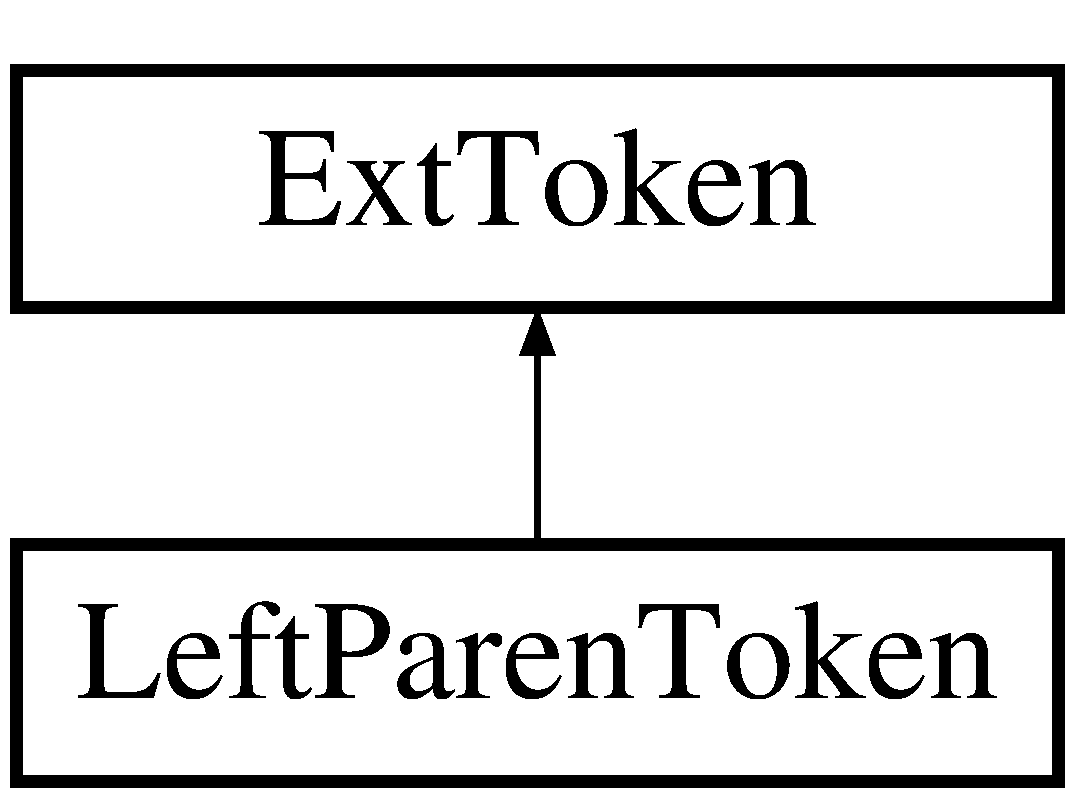
\includegraphics[height=2.000000cm]{classLeftParenToken}
\end{center}
\end{figure}
\subsection*{Public Member Functions}
\begin{DoxyCompactItemize}
\item 
\hypertarget{classLeftParenToken_aecdc6faf48a1a7192ec55712f0264cba}{{\bfseries Left\-Paren\-Token} (\hyperlink{classParser}{Parser} $\ast$p, \hyperlink{classToken}{Token} $\ast$t)}\label{classLeftParenToken_aecdc6faf48a1a7192ec55712f0264cba}

\item 
\hypertarget{classLeftParenToken_a3cb3ae9ab2647e5534c85529d314f08b}{\hyperlink{classParseResult}{Parse\-Result} {\bfseries nud} ()}\label{classLeftParenToken_a3cb3ae9ab2647e5534c85529d314f08b}

\item 
\hypertarget{classLeftParenToken_a2df35684bd2081c3bdfe2357946917bc}{std\-::string {\bfseries description} ()}\label{classLeftParenToken_a2df35684bd2081c3bdfe2357946917bc}

\item 
\hypertarget{classLeftParenToken_afa1b94645278f097bb097d3b24445d14}{int {\bfseries lbp} ()}\label{classLeftParenToken_afa1b94645278f097bb097d3b24445d14}

\end{DoxyCompactItemize}
\subsection*{Additional Inherited Members}


The documentation for this class was generated from the following file\-:\begin{DoxyCompactItemize}
\item 
ext\-Token.\-h\end{DoxyCompactItemize}

\hypertarget{classLetExpr}{\section{Let\-Expr Class Reference}
\label{classLetExpr}\index{Let\-Expr@{Let\-Expr}}
}


\hyperlink{classExpr}{Expr} \-:\-:= 'let' \hyperlink{classStmts}{Stmts} 'in' \hyperlink{classExpr}{Expr} 'end' //\-Let\-Expr.  




{\ttfamily \#include $<$A\-S\-T.\-h$>$}

Inheritance diagram for Let\-Expr\-:\begin{figure}[H]
\begin{center}
\leavevmode
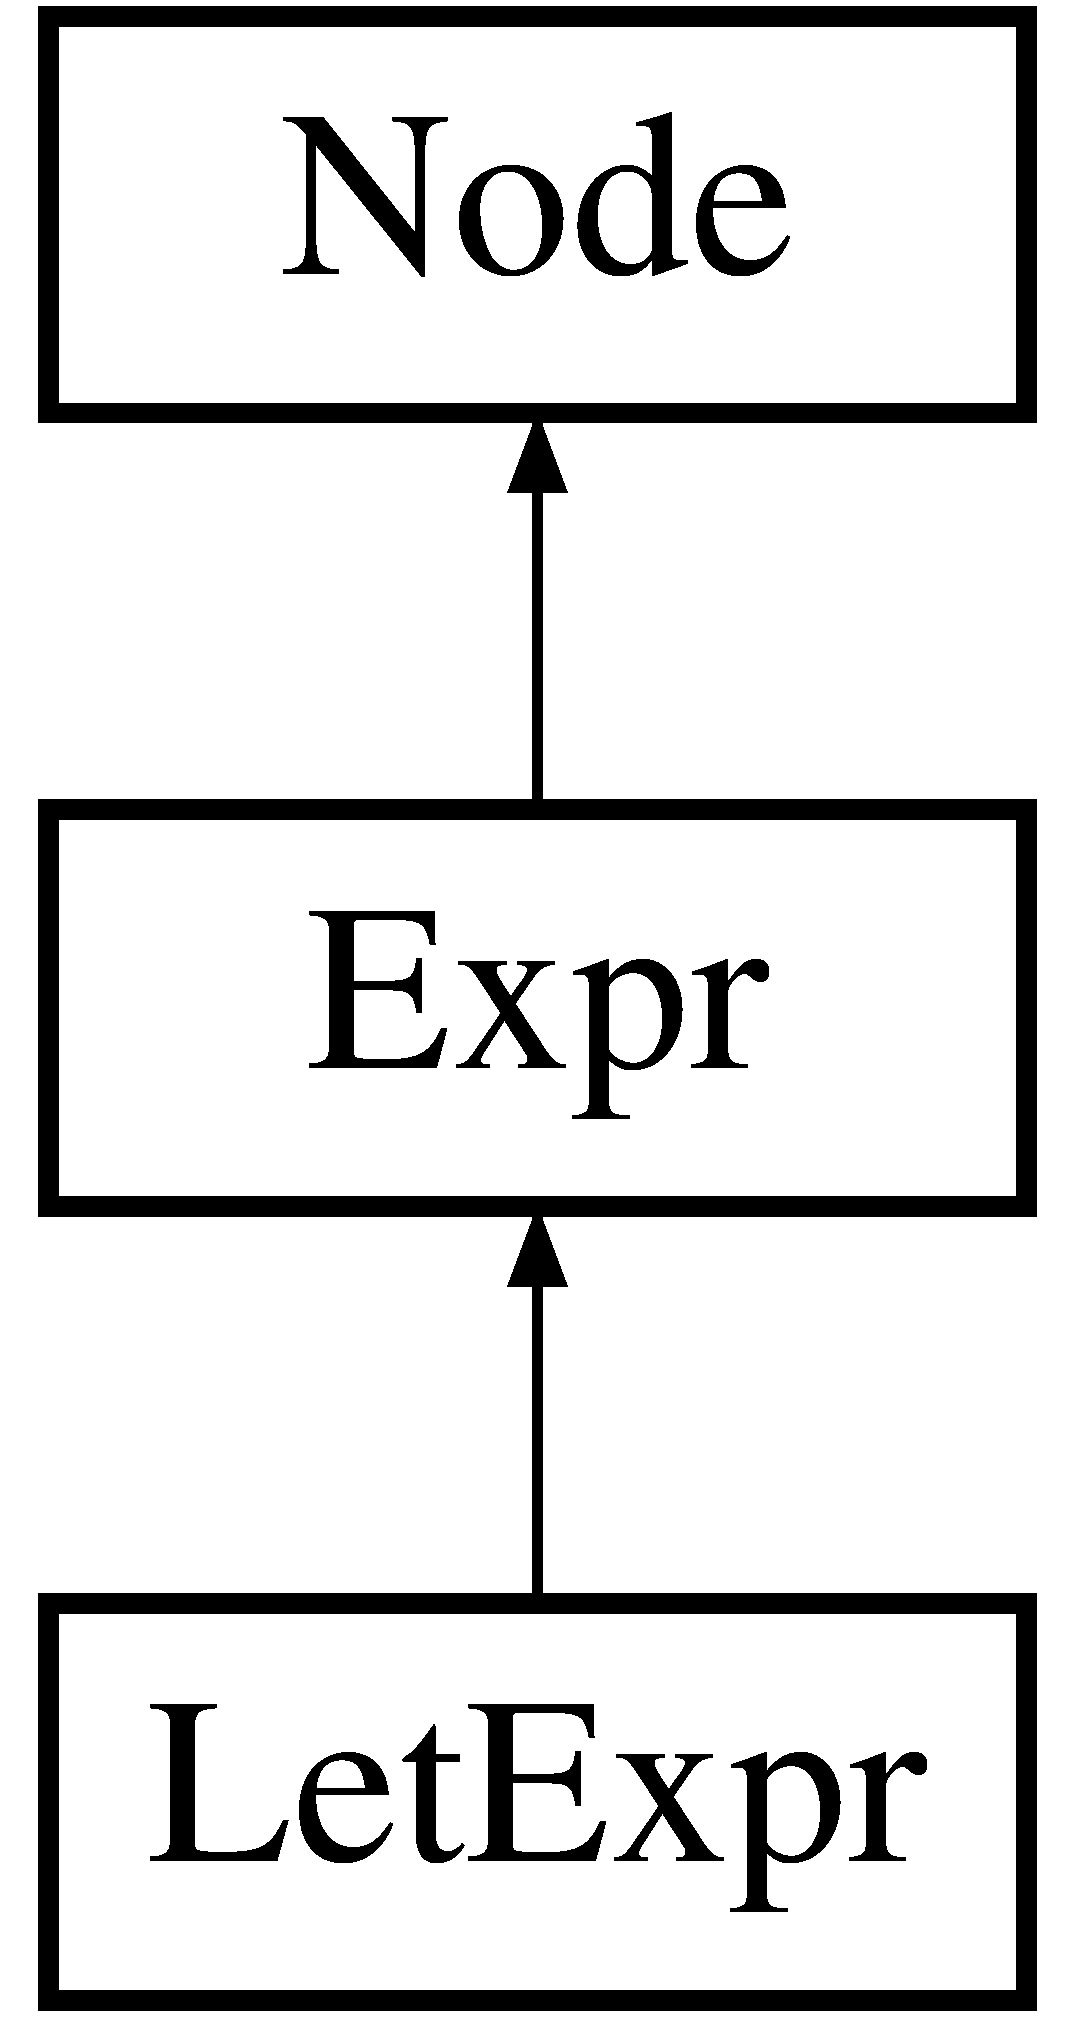
\includegraphics[height=3.000000cm]{classLetExpr}
\end{center}
\end{figure}
\subsection*{Public Member Functions}
\begin{DoxyCompactItemize}
\item 
\hypertarget{classLetExpr_a73ee0ccb9d07cdccc88e90d567f9951f}{{\bfseries Let\-Expr} (\hyperlink{classStmts}{Stmts} $\ast$ss, \hyperlink{classExpr}{Expr} $\ast$e)}\label{classLetExpr_a73ee0ccb9d07cdccc88e90d567f9951f}

\item 
\hypertarget{classLetExpr_a47e9e62ebec3114d50c127223fff126b}{std\-::string \hyperlink{classLetExpr_a47e9e62ebec3114d50c127223fff126b}{unparse} ()}\label{classLetExpr_a47e9e62ebec3114d50c127223fff126b}

\begin{DoxyCompactList}\small\item\em Unparse in proper 'Let \hyperlink{classExpr}{Expr}' form as denoted in grammar. \end{DoxyCompactList}\end{DoxyCompactItemize}


\subsection{Detailed Description}
\hyperlink{classExpr}{Expr} \-:\-:= 'let' \hyperlink{classStmts}{Stmts} 'in' \hyperlink{classExpr}{Expr} 'end' //\-Let\-Expr. 

The documentation for this class was generated from the following file\-:\begin{DoxyCompactItemize}
\item 
A\-S\-T.\-h\end{DoxyCompactItemize}

\hypertarget{classLetToken}{\section{Let\-Token Class Reference}
\label{classLetToken}\index{Let\-Token@{Let\-Token}}
}
Inheritance diagram for Let\-Token\-:\begin{figure}[H]
\begin{center}
\leavevmode
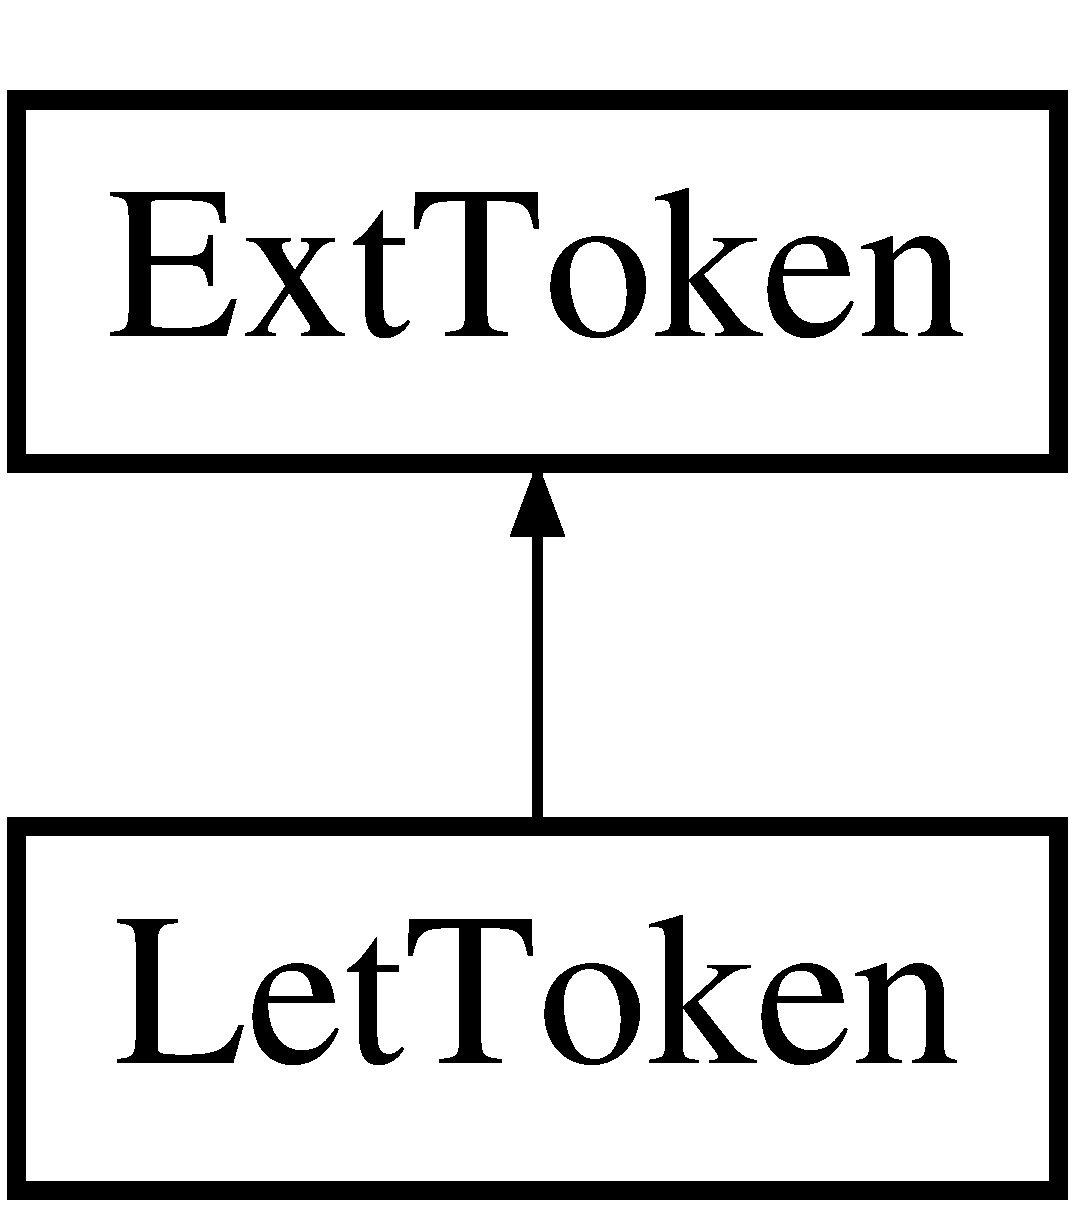
\includegraphics[height=2.000000cm]{classLetToken}
\end{center}
\end{figure}
\subsection*{Public Member Functions}
\begin{DoxyCompactItemize}
\item 
\hypertarget{classLetToken_a94651a82207e47cd2c1066a58cb1fe08}{{\bfseries Let\-Token} (\hyperlink{classParser}{Parser} $\ast$p, \hyperlink{classToken}{Token} $\ast$t)}\label{classLetToken_a94651a82207e47cd2c1066a58cb1fe08}

\item 
\hypertarget{classLetToken_a14df948cdf775bde8392bf58d53b91f3}{\hyperlink{classParseResult}{Parse\-Result} {\bfseries nud} ()}\label{classLetToken_a14df948cdf775bde8392bf58d53b91f3}

\item 
\hypertarget{classLetToken_a2c5ba0489774bf6468a26f4e19d7fab4}{std\-::string {\bfseries description} ()}\label{classLetToken_a2c5ba0489774bf6468a26f4e19d7fab4}

\item 
\hypertarget{classLetToken_a2a5ab5bc5897340513480c162bb2b065}{int {\bfseries lbp} ()}\label{classLetToken_a2a5ab5bc5897340513480c162bb2b065}

\end{DoxyCompactItemize}
\subsection*{Additional Inherited Members}


The documentation for this class was generated from the following file\-:\begin{DoxyCompactItemize}
\item 
ext\-Token.\-h\end{DoxyCompactItemize}

\hypertarget{classLogicOperator}{\section{Logic\-Operator Class Reference}
\label{classLogicOperator}\index{Logic\-Operator@{Logic\-Operator}}
}


Handles logic operators ($>$, $>$=, $<$, $<$=, ==, !=, \&\&, $\vert$$\vert$)  




{\ttfamily \#include $<$A\-S\-T.\-h$>$}

Inheritance diagram for Logic\-Operator\-:\begin{figure}[H]
\begin{center}
\leavevmode
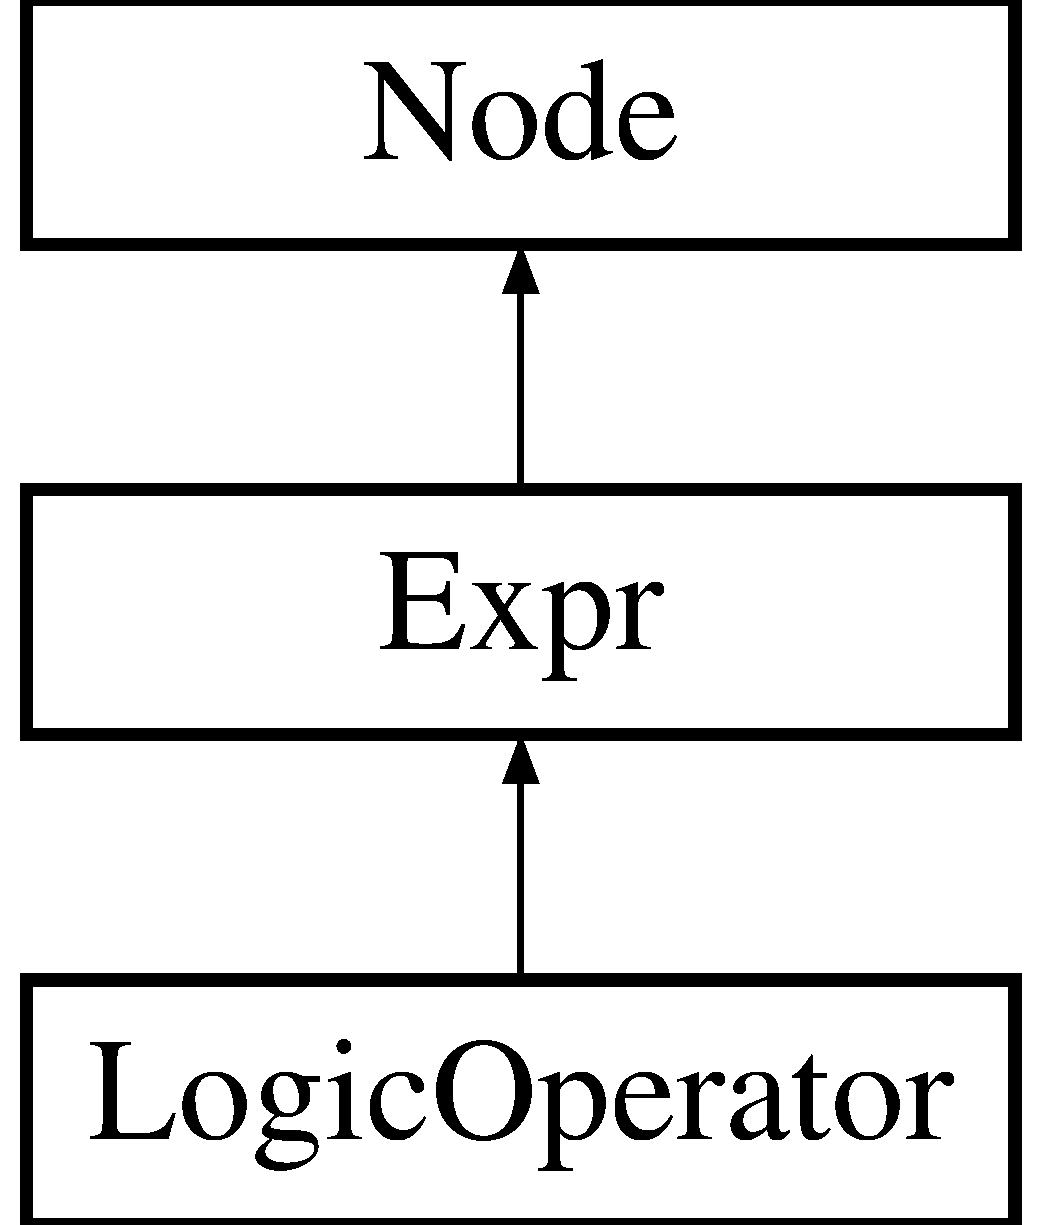
\includegraphics[height=3.000000cm]{classLogicOperator}
\end{center}
\end{figure}
\subsection*{Public Member Functions}
\begin{DoxyCompactItemize}
\item 
\hypertarget{classLogicOperator_a2087e8fe4e93fcdbafd22ae776132cae}{{\bfseries Logic\-Operator} (\hyperlink{classExpr}{Expr} $\ast$e1, std\-::string op, \hyperlink{classExpr}{Expr} $\ast$e2)}\label{classLogicOperator_a2087e8fe4e93fcdbafd22ae776132cae}

\item 
\hypertarget{classLogicOperator_a43c2cc6c8999c69c561e93f262a87da9}{std\-::string \hyperlink{classLogicOperator_a43c2cc6c8999c69c561e93f262a87da9}{unparse} ()}\label{classLogicOperator_a43c2cc6c8999c69c561e93f262a87da9}

\begin{DoxyCompactList}\small\item\em Unparse expression one and expression two separated by the proper logic operator. \end{DoxyCompactList}\end{DoxyCompactItemize}


\subsection{Detailed Description}
Handles logic operators ($>$, $>$=, $<$, $<$=, ==, !=, \&\&, $\vert$$\vert$) 

The documentation for this class was generated from the following file\-:\begin{DoxyCompactItemize}
\item 
A\-S\-T.\-h\end{DoxyCompactItemize}

\hypertarget{classMatrixDecl1}{\section{Matrix\-Decl1 Class Reference}
\label{classMatrixDecl1}\index{Matrix\-Decl1@{Matrix\-Decl1}}
}


\hyperlink{classDecl}{Decl} \-:\-:= 'matrix' var\-Name '\mbox{[}' \hyperlink{classExpr}{Expr} '\-:' \hyperlink{classExpr}{Expr} '\mbox{]}' var\-Name '\-:' var\-Name '=' \hyperlink{classExpr}{Expr} ';'.  




{\ttfamily \#include $<$A\-S\-T.\-h$>$}

Inheritance diagram for Matrix\-Decl1\-:\begin{figure}[H]
\begin{center}
\leavevmode
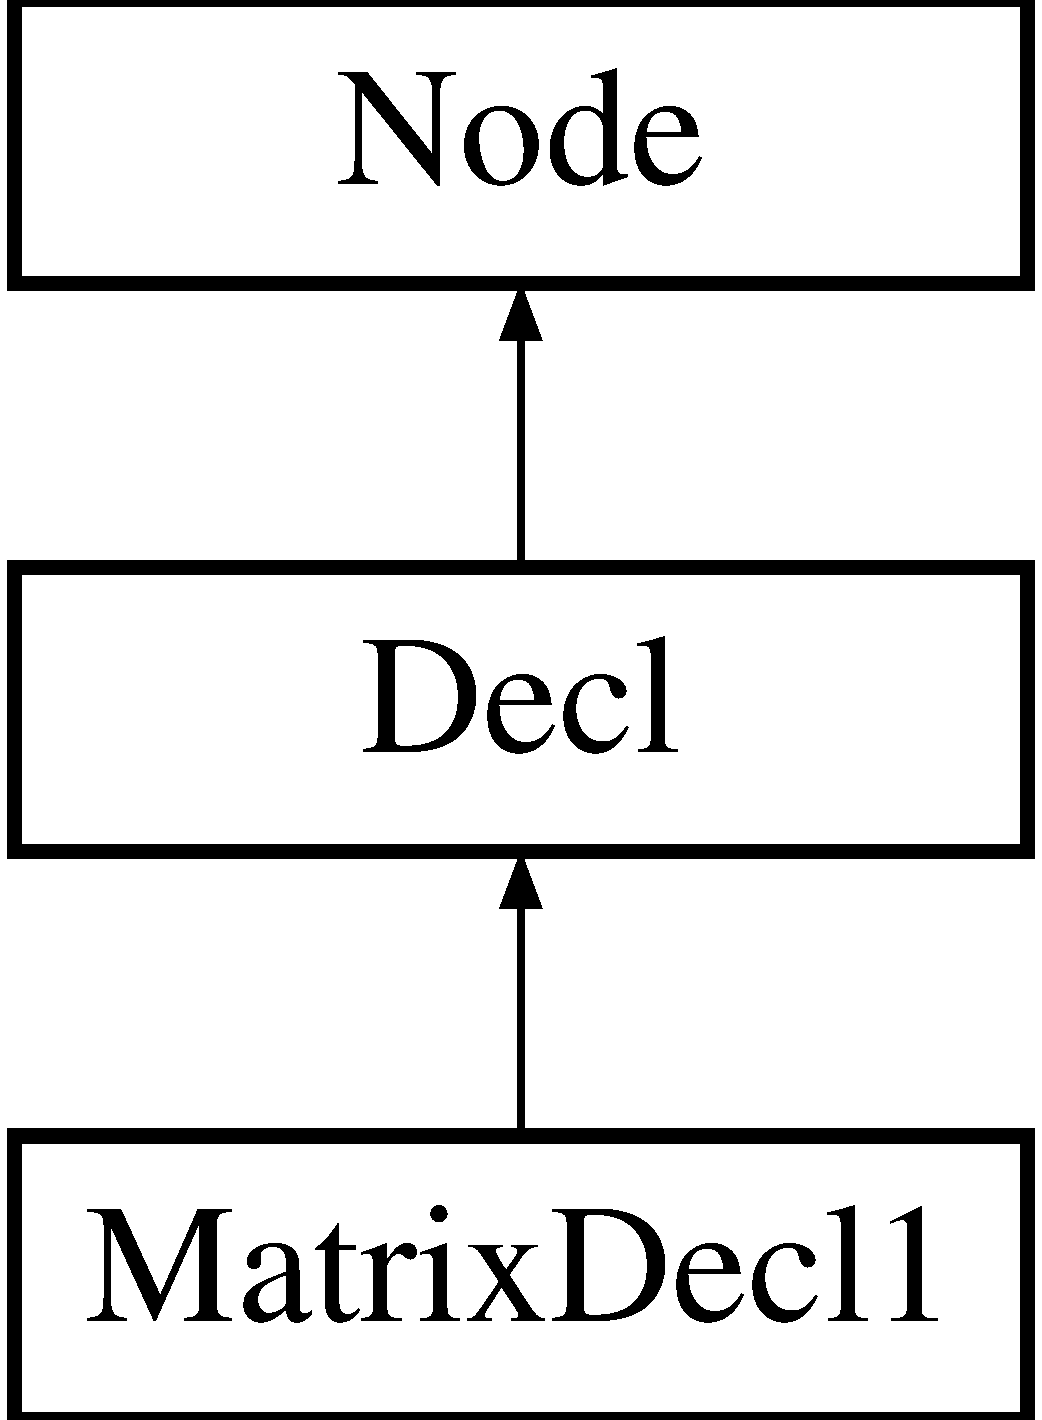
\includegraphics[height=3.000000cm]{classMatrixDecl1}
\end{center}
\end{figure}
\subsection*{Public Member Functions}
\begin{DoxyCompactItemize}
\item 
\hypertarget{classMatrixDecl1_a863346bc697d7ca06262e80c7b3a48bd}{{\bfseries Matrix\-Decl1} (\hyperlink{classExpr}{Expr} $\ast$v1, \hyperlink{classExpr}{Expr} $\ast$e1, \hyperlink{classExpr}{Expr} $\ast$e2, \hyperlink{classExpr}{Expr} $\ast$v2, \hyperlink{classExpr}{Expr} $\ast$v3, \hyperlink{classExpr}{Expr} $\ast$e3)}\label{classMatrixDecl1_a863346bc697d7ca06262e80c7b3a48bd}

\item 
\hypertarget{classMatrixDecl1_a01beb5e497f7752612d396d3ca3f7bca}{std\-::string \hyperlink{classMatrixDecl1_a01beb5e497f7752612d396d3ca3f7bca}{unparse} ()}\label{classMatrixDecl1_a01beb5e497f7752612d396d3ca3f7bca}

\begin{DoxyCompactList}\small\item\em Unparse in proper 'matrix declaration' version 1 form as denoted in grammar. \end{DoxyCompactList}\end{DoxyCompactItemize}


\subsection{Detailed Description}
\hyperlink{classDecl}{Decl} \-:\-:= 'matrix' var\-Name '\mbox{[}' \hyperlink{classExpr}{Expr} '\-:' \hyperlink{classExpr}{Expr} '\mbox{]}' var\-Name '\-:' var\-Name '=' \hyperlink{classExpr}{Expr} ';'. 

The documentation for this class was generated from the following file\-:\begin{DoxyCompactItemize}
\item 
A\-S\-T.\-h\end{DoxyCompactItemize}

\hypertarget{classMatrixDecl2}{\section{Matrix\-Decl2 Class Reference}
\label{classMatrixDecl2}\index{Matrix\-Decl2@{Matrix\-Decl2}}
}


\hyperlink{classDecl}{Decl} \-:\-:= 'matrix' var\-Name '=' \hyperlink{classExpr}{Expr} ';'.  




{\ttfamily \#include $<$A\-S\-T.\-h$>$}

Inheritance diagram for Matrix\-Decl2\-:\begin{figure}[H]
\begin{center}
\leavevmode
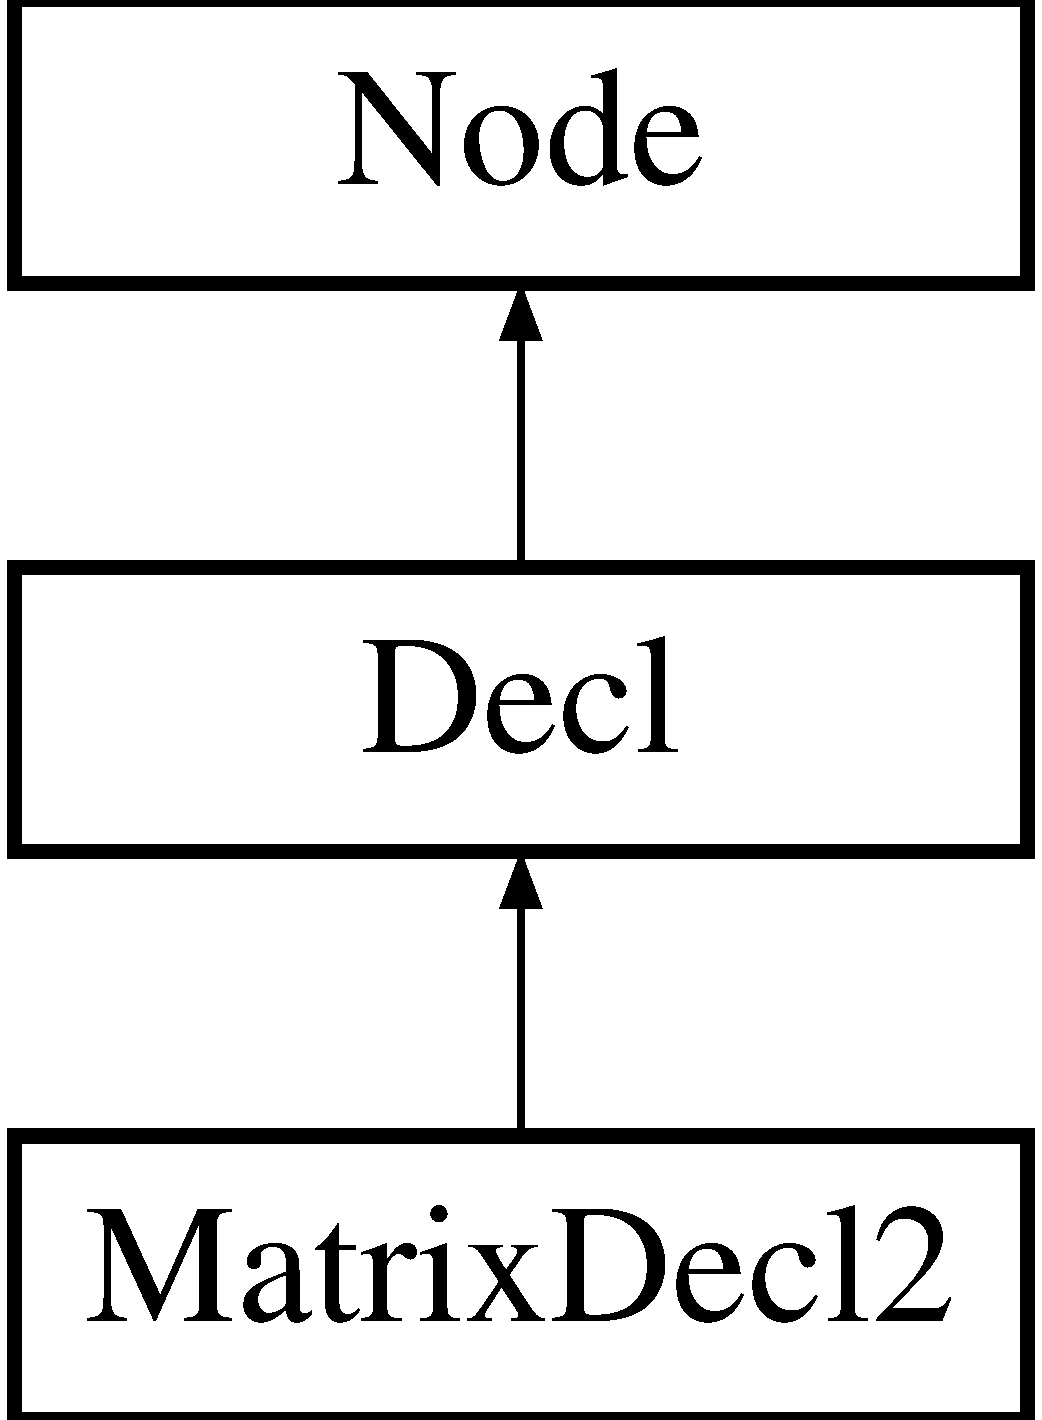
\includegraphics[height=3.000000cm]{classMatrixDecl2}
\end{center}
\end{figure}
\subsection*{Public Member Functions}
\begin{DoxyCompactItemize}
\item 
\hypertarget{classMatrixDecl2_aca5dfa8bd7c19a2ce63463245d708dd9}{{\bfseries Matrix\-Decl2} (\hyperlink{classExpr}{Expr} $\ast$v, \hyperlink{classExpr}{Expr} $\ast$e)}\label{classMatrixDecl2_aca5dfa8bd7c19a2ce63463245d708dd9}

\item 
\hypertarget{classMatrixDecl2_ac6c560f16e2f8b032fb1d34274d44c84}{std\-::string \hyperlink{classMatrixDecl2_ac6c560f16e2f8b032fb1d34274d44c84}{unparse} ()}\label{classMatrixDecl2_ac6c560f16e2f8b032fb1d34274d44c84}

\begin{DoxyCompactList}\small\item\em Unparse in proper 'matrix declaration' version 2 form as denoted in grammar. \end{DoxyCompactList}\end{DoxyCompactItemize}


\subsection{Detailed Description}
\hyperlink{classDecl}{Decl} \-:\-:= 'matrix' var\-Name '=' \hyperlink{classExpr}{Expr} ';'. 

The documentation for this class was generated from the following file\-:\begin{DoxyCompactItemize}
\item 
A\-S\-T.\-h\end{DoxyCompactItemize}

\hypertarget{classMatrixRef}{\section{Matrix\-Ref Class Reference}
\label{classMatrixRef}\index{Matrix\-Ref@{Matrix\-Ref}}
}


\hyperlink{classExpr}{Expr} \-:\-:= var\-Name '\mbox{[}' \hyperlink{classExpr}{Expr} '\-:' \hyperlink{classExpr}{Expr} '\mbox{]}' //\-Matrix\-R\-Ef.  




{\ttfamily \#include $<$A\-S\-T.\-h$>$}

Inheritance diagram for Matrix\-Ref\-:\begin{figure}[H]
\begin{center}
\leavevmode
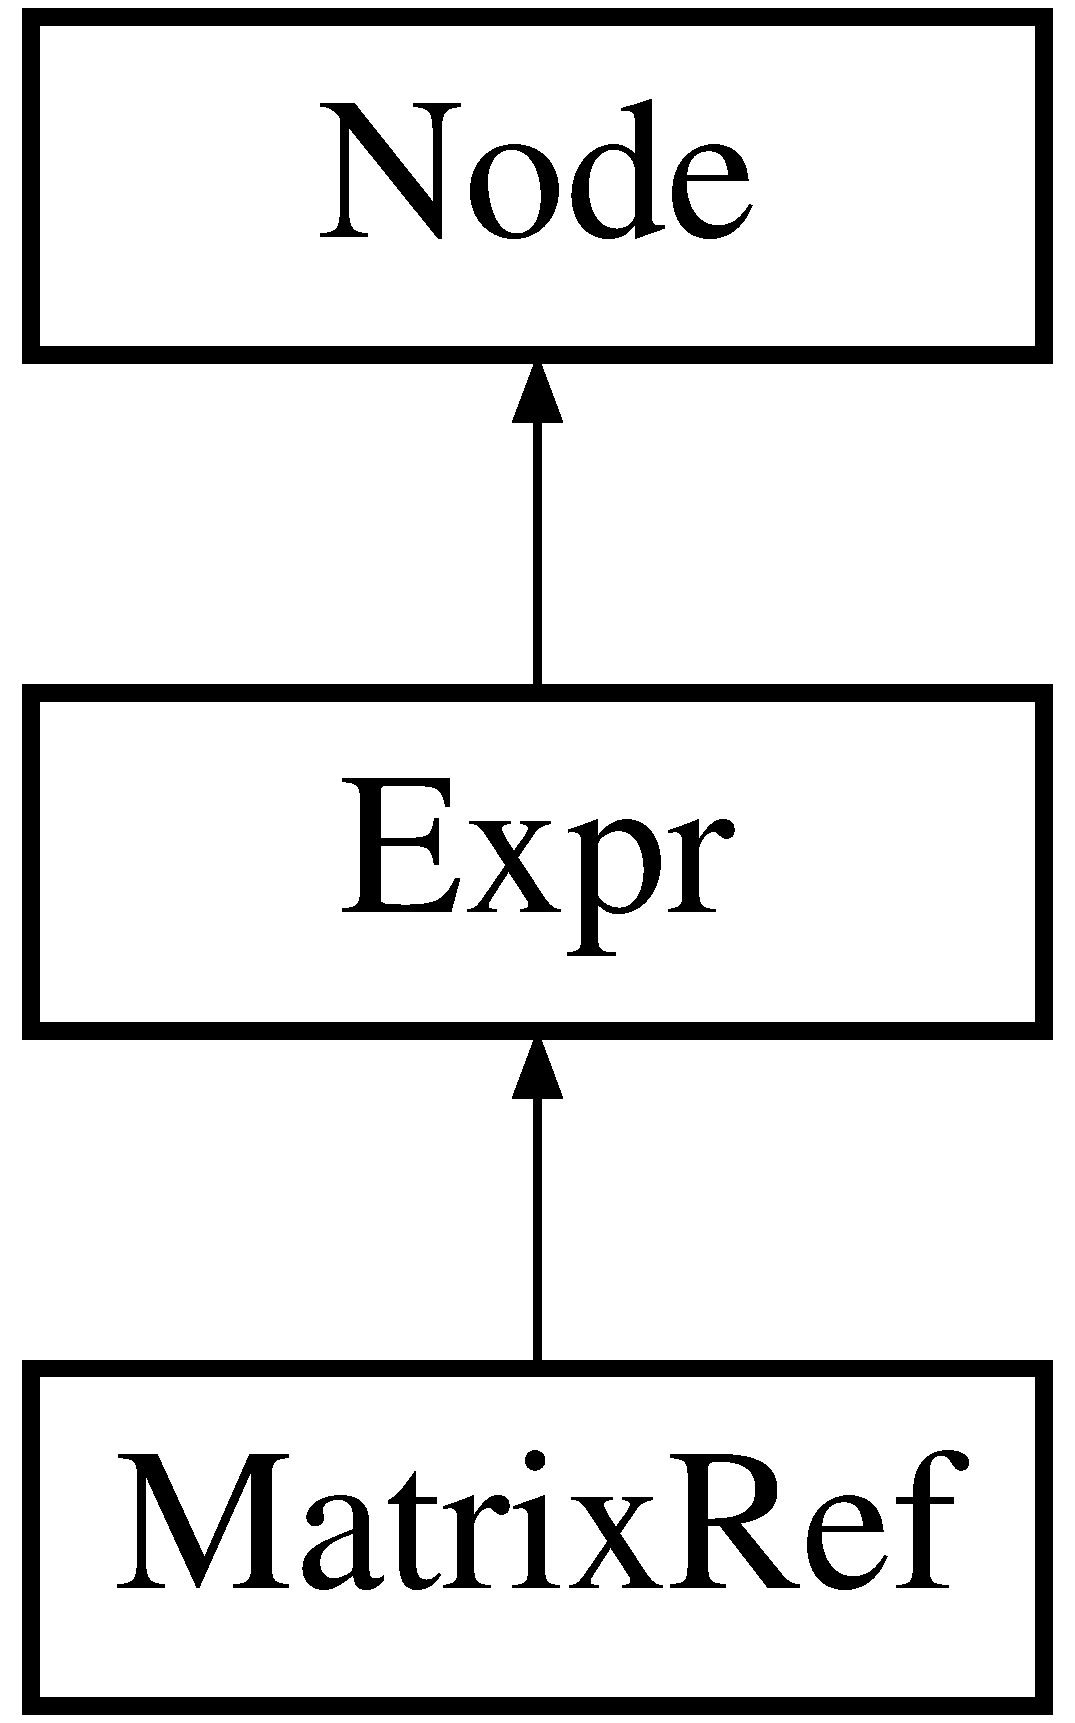
\includegraphics[height=3.000000cm]{classMatrixRef}
\end{center}
\end{figure}
\subsection*{Public Member Functions}
\begin{DoxyCompactItemize}
\item 
\hypertarget{classMatrixRef_a369a1da63af501e2dfe6c62c54f5dd28}{{\bfseries Matrix\-Ref} (\hyperlink{classExpr}{Expr} $\ast$v, \hyperlink{classExpr}{Expr} $\ast$e1, \hyperlink{classExpr}{Expr} $\ast$e2)}\label{classMatrixRef_a369a1da63af501e2dfe6c62c54f5dd28}

\item 
\hypertarget{classMatrixRef_aedf083a71a74fec22264aa71fdedb5e6}{std\-::string \hyperlink{classMatrixRef_aedf083a71a74fec22264aa71fdedb5e6}{unparse} ()}\label{classMatrixRef_aedf083a71a74fec22264aa71fdedb5e6}

\begin{DoxyCompactList}\small\item\em Unparse in proper 'Matrix Ref' form as denoted in grammar. \end{DoxyCompactList}\end{DoxyCompactItemize}


\subsection{Detailed Description}
\hyperlink{classExpr}{Expr} \-:\-:= var\-Name '\mbox{[}' \hyperlink{classExpr}{Expr} '\-:' \hyperlink{classExpr}{Expr} '\mbox{]}' //\-Matrix\-R\-Ef. 

The documentation for this class was generated from the following file\-:\begin{DoxyCompactItemize}
\item 
A\-S\-T.\-h\end{DoxyCompactItemize}

\hypertarget{classNestedOrFuncCall}{\section{Nested\-Or\-Func\-Call Class Reference}
\label{classNestedOrFuncCall}\index{Nested\-Or\-Func\-Call@{Nested\-Or\-Func\-Call}}
}


\hyperlink{classExpr}{Expr} \-:\-:= var\-Name '(' \hyperlink{classExpr}{Expr} ')' //\-Nested\-Or\-Function\-Call.  




{\ttfamily \#include $<$A\-S\-T.\-h$>$}

Inheritance diagram for Nested\-Or\-Func\-Call\-:\begin{figure}[H]
\begin{center}
\leavevmode
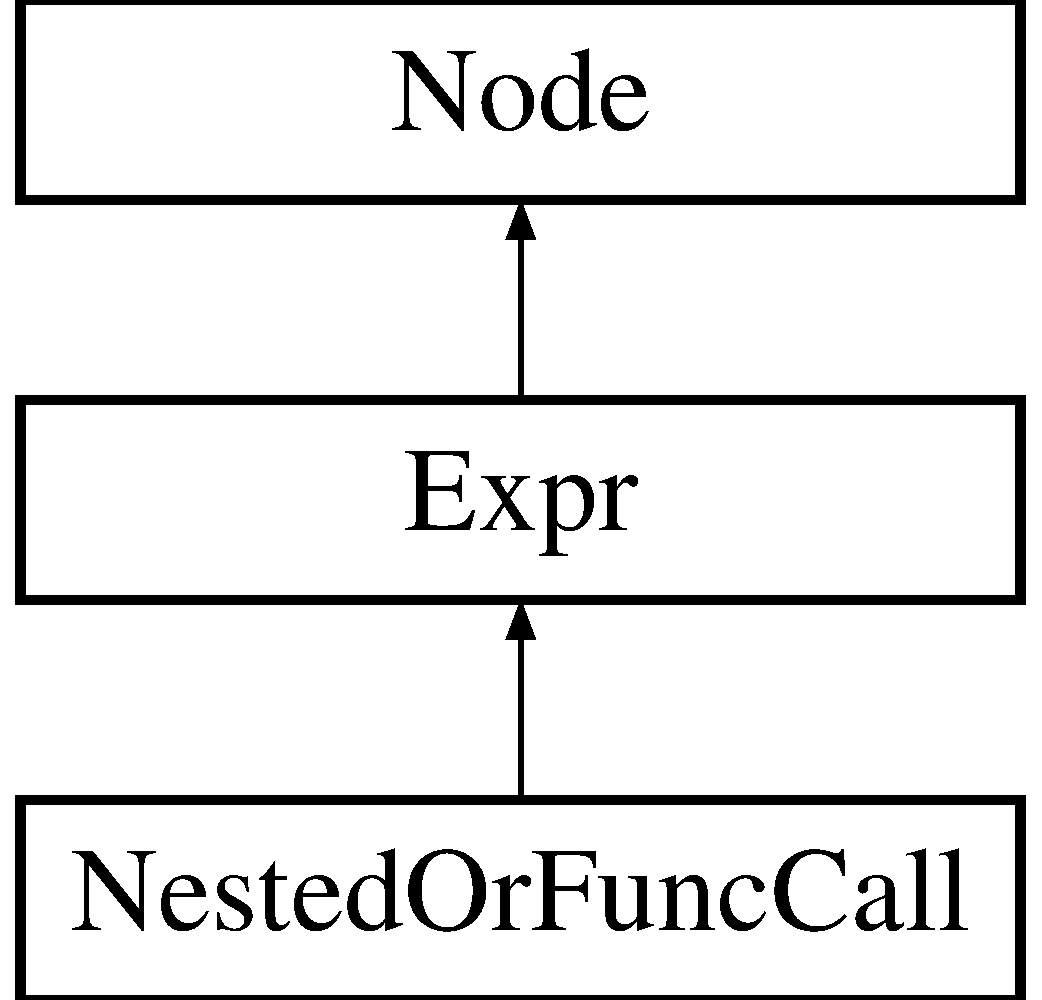
\includegraphics[height=3.000000cm]{classNestedOrFuncCall}
\end{center}
\end{figure}
\subsection*{Public Member Functions}
\begin{DoxyCompactItemize}
\item 
\hypertarget{classNestedOrFuncCall_ad6a1ea0a0646a8e9abc04747414287a6}{{\bfseries Nested\-Or\-Func\-Call} (\hyperlink{classExpr}{Expr} $\ast$v, \hyperlink{classExpr}{Expr} $\ast$e)}\label{classNestedOrFuncCall_ad6a1ea0a0646a8e9abc04747414287a6}

\item 
\hypertarget{classNestedOrFuncCall_a6d24500653da39566c63538439742cd3}{std\-::string \hyperlink{classNestedOrFuncCall_a6d24500653da39566c63538439742cd3}{unparse} ()}\label{classNestedOrFuncCall_a6d24500653da39566c63538439742cd3}

\begin{DoxyCompactList}\small\item\em Unparse in proper 'Nested Or Function Call' form as denoted in grammar. \end{DoxyCompactList}\end{DoxyCompactItemize}


\subsection{Detailed Description}
\hyperlink{classExpr}{Expr} \-:\-:= var\-Name '(' \hyperlink{classExpr}{Expr} ')' //\-Nested\-Or\-Function\-Call. 

The documentation for this class was generated from the following file\-:\begin{DoxyCompactItemize}
\item 
A\-S\-T.\-h\end{DoxyCompactItemize}

\hypertarget{classNode}{\section{Node Class Reference}
\label{classNode}\index{Node@{Node}}
}


\hyperlink{classNode}{Node}.  




{\ttfamily \#include $<$A\-S\-T.\-h$>$}

Inheritance diagram for Node\-:\begin{figure}[H]
\begin{center}
\leavevmode
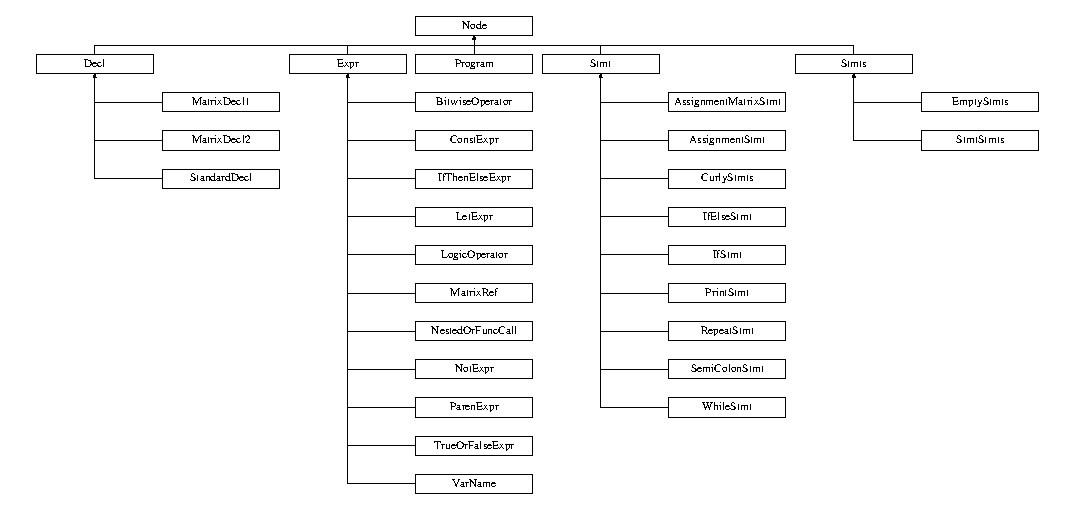
\includegraphics[height=6.408450cm]{classNode}
\end{center}
\end{figure}
\subsection*{Public Member Functions}
\begin{DoxyCompactItemize}
\item 
virtual std\-::string \hyperlink{classNode_aeb327c708aa4acd82d0f11a9620f0ae8}{unparse} ()
\item 
\hypertarget{classNode_ab9dc8a0791d329231bc8427a7d7e9c2f}{virtual std\-::string {\bfseries cpp\-Code} ()}\label{classNode_ab9dc8a0791d329231bc8427a7d7e9c2f}

\end{DoxyCompactItemize}


\subsection{Detailed Description}
\hyperlink{classNode}{Node}. 

\subsection{Member Function Documentation}
\hypertarget{classNode_aeb327c708aa4acd82d0f11a9620f0ae8}{\index{Node@{Node}!unparse@{unparse}}
\index{unparse@{unparse}!Node@{Node}}
\subsubsection[{unparse}]{\setlength{\rightskip}{0pt plus 5cm}virtual std\-::string Node\-::unparse (
\begin{DoxyParamCaption}
{}
\end{DoxyParamCaption}
)\hspace{0.3cm}{\ttfamily [inline]}, {\ttfamily [virtual]}}}\label{classNode_aeb327c708aa4acd82d0f11a9620f0ae8}
The unparse method is inherited by each class. This node return should never execute. 

Reimplemented in \hyperlink{classNotExpr_ab49f96d8f23e3fa6bb21376dc0fa5215}{Not\-Expr}, \hyperlink{classIfThenElseExpr_a1686a9926fe0017d7cf8dd86c7ab79a0}{If\-Then\-Else\-Expr}, \hyperlink{classLetExpr_a47e9e62ebec3114d50c127223fff126b}{Let\-Expr}, \hyperlink{classParenExpr_a894bdf8546f0242c85b4664a2f9492cd}{Paren\-Expr}, \hyperlink{classNestedOrFuncCall_a6d24500653da39566c63538439742cd3}{Nested\-Or\-Func\-Call}, \hyperlink{classMatrixRef_aedf083a71a74fec22264aa71fdedb5e6}{Matrix\-Ref}, \hyperlink{classLogicOperator_a43c2cc6c8999c69c561e93f262a87da9}{Logic\-Operator}, \hyperlink{classBitwiseOperator_aab4c8032951100835bdcebf08e924e5e}{Bitwise\-Operator}, \hyperlink{classTrueOrFalseExpr_a3b981c8f3803f2a2520c7feef1d0ca0b}{True\-Or\-False\-Expr}, \hyperlink{classConstExpr_adc01f00000a931c663aedffdfcd132ad}{Const\-Expr}, \hyperlink{classMatrixDecl2_ac6c560f16e2f8b032fb1d34274d44c84}{Matrix\-Decl2}, \hyperlink{classMatrixDecl1_a01beb5e497f7752612d396d3ca3f7bca}{Matrix\-Decl1}, \hyperlink{classStandardDecl_a2666e01d836103d4a4338a2c54106db5}{Standard\-Decl}, \hyperlink{classSemiColonStmt_a210b082574bda3fa4b408f0022987501}{Semi\-Colon\-Stmt}, \hyperlink{classWhileStmt_acf3bd2eb99735445a3f8b0e2faa27a29}{While\-Stmt}, \hyperlink{classRepeatStmt_a9ccc876694fd9b60671818bb9c81447e}{Repeat\-Stmt}, \hyperlink{classPrintStmt_aa3c9ad246b75bd45a48e563500b5109f}{Print\-Stmt}, \hyperlink{classAssignmentMatrixStmt_adbdf4dee03753d6a0a098cf3a9eff6a8}{Assignment\-Matrix\-Stmt}, \hyperlink{classAssignmentStmt_a892c33dd7fa55fda0f85ced1b5684f98}{Assignment\-Stmt}, \hyperlink{classIfElseStmt_a82267559f8fdd5f10cf14e616f3867f2}{If\-Else\-Stmt}, \hyperlink{classIfStmt_a615e8785edb068f24e19f3ce7863f2ce}{If\-Stmt}, \hyperlink{classCurlyStmts_af141e51f7aede8f95d094f9d91839666}{Curly\-Stmts}, \hyperlink{classEmptyStmts_a127064ef5c59227fc8452b31c65eb905}{Empty\-Stmts}, \hyperlink{classStmtStmts_a834f10443d4c197b5741a00395f787eb}{Stmt\-Stmts}, \hyperlink{classProgram_a33c78e36a63c63e5821b7747bec7b644}{Program}, and \hyperlink{classVarName_af29612051468cad25343614de9bb067f}{Var\-Name}.



The documentation for this class was generated from the following file\-:\begin{DoxyCompactItemize}
\item 
A\-S\-T.\-h\end{DoxyCompactItemize}

\hypertarget{classNotExpr}{\section{Not\-Expr Class Reference}
\label{classNotExpr}\index{Not\-Expr@{Not\-Expr}}
}


\hyperlink{classExpr}{Expr} \-:\-:= '!' \hyperlink{classExpr}{Expr}.  




{\ttfamily \#include $<$A\-S\-T.\-h$>$}

Inheritance diagram for Not\-Expr\-:\begin{figure}[H]
\begin{center}
\leavevmode
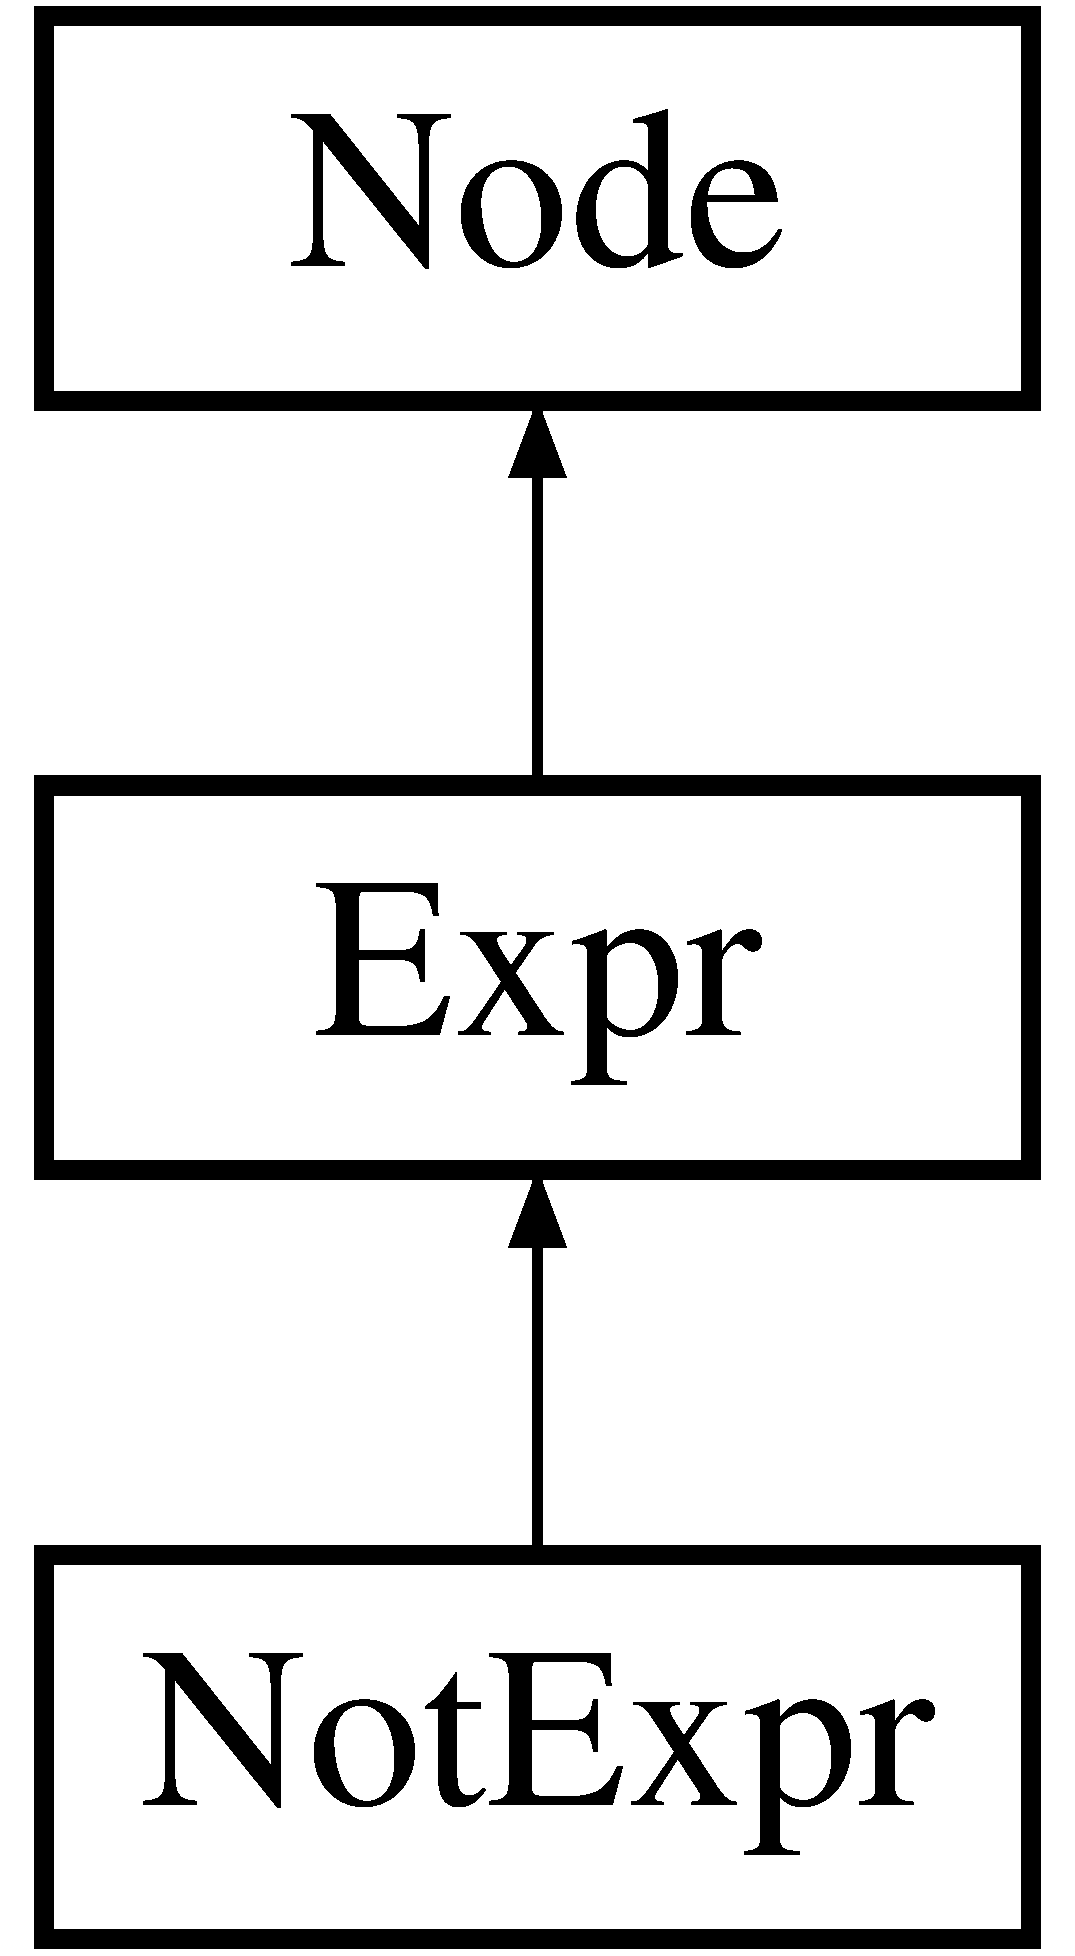
\includegraphics[height=3.000000cm]{classNotExpr}
\end{center}
\end{figure}
\subsection*{Public Member Functions}
\begin{DoxyCompactItemize}
\item 
\hypertarget{classNotExpr_a7939cb5c7141f8ede498cef1e8f9694c}{{\bfseries Not\-Expr} (\hyperlink{classExpr}{Expr} $\ast$e)}\label{classNotExpr_a7939cb5c7141f8ede498cef1e8f9694c}

\item 
\hypertarget{classNotExpr_ab49f96d8f23e3fa6bb21376dc0fa5215}{std\-::string \hyperlink{classNotExpr_ab49f96d8f23e3fa6bb21376dc0fa5215}{unparse} ()}\label{classNotExpr_ab49f96d8f23e3fa6bb21376dc0fa5215}

\begin{DoxyCompactList}\small\item\em Unparse exclamation mark followed by the expression. \end{DoxyCompactList}\end{DoxyCompactItemize}


\subsection{Detailed Description}
\hyperlink{classExpr}{Expr} \-:\-:= '!' \hyperlink{classExpr}{Expr}. 

The documentation for this class was generated from the following file\-:\begin{DoxyCompactItemize}
\item 
A\-S\-T.\-h\end{DoxyCompactItemize}

\hypertarget{classNotOpToken}{\section{Not\-Op\-Token Class Reference}
\label{classNotOpToken}\index{Not\-Op\-Token@{Not\-Op\-Token}}
}
Inheritance diagram for Not\-Op\-Token\-:\begin{figure}[H]
\begin{center}
\leavevmode
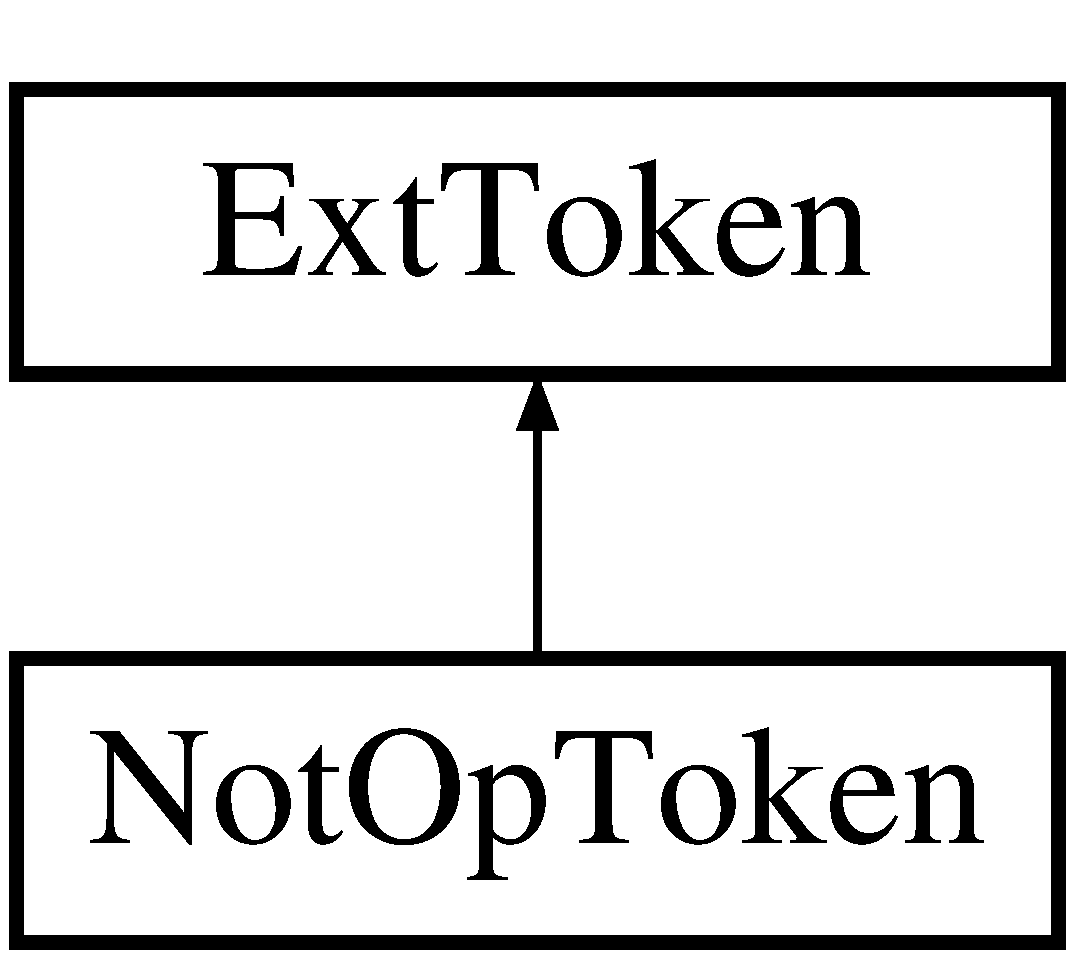
\includegraphics[height=2.000000cm]{classNotOpToken}
\end{center}
\end{figure}
\subsection*{Public Member Functions}
\begin{DoxyCompactItemize}
\item 
\hypertarget{classNotOpToken_afb8b9e96a178b1dfd69abf0a901dfddf}{{\bfseries Not\-Op\-Token} (\hyperlink{classParser}{Parser} $\ast$p, \hyperlink{classToken}{Token} $\ast$t)}\label{classNotOpToken_afb8b9e96a178b1dfd69abf0a901dfddf}

\item 
\hypertarget{classNotOpToken_a55a0dd53742aaca04338c16be079b031}{\hyperlink{classParseResult}{Parse\-Result} {\bfseries nud} ()}\label{classNotOpToken_a55a0dd53742aaca04338c16be079b031}

\item 
\hypertarget{classNotOpToken_a136a11f1e42542a9a58b7c14249c9d23}{std\-::string {\bfseries description} ()}\label{classNotOpToken_a136a11f1e42542a9a58b7c14249c9d23}

\end{DoxyCompactItemize}
\subsection*{Additional Inherited Members}


The documentation for this class was generated from the following file\-:\begin{DoxyCompactItemize}
\item 
ext\-Token.\-h\end{DoxyCompactItemize}

\hypertarget{classParenExpr}{\section{Paren\-Expr Class Reference}
\label{classParenExpr}\index{Paren\-Expr@{Paren\-Expr}}
}


\hyperlink{classExpr}{Expr} \-:\-:= '(' \hyperlink{classExpr}{Expr} ')'.  




{\ttfamily \#include $<$A\-S\-T.\-h$>$}

Inheritance diagram for Paren\-Expr\-:\begin{figure}[H]
\begin{center}
\leavevmode
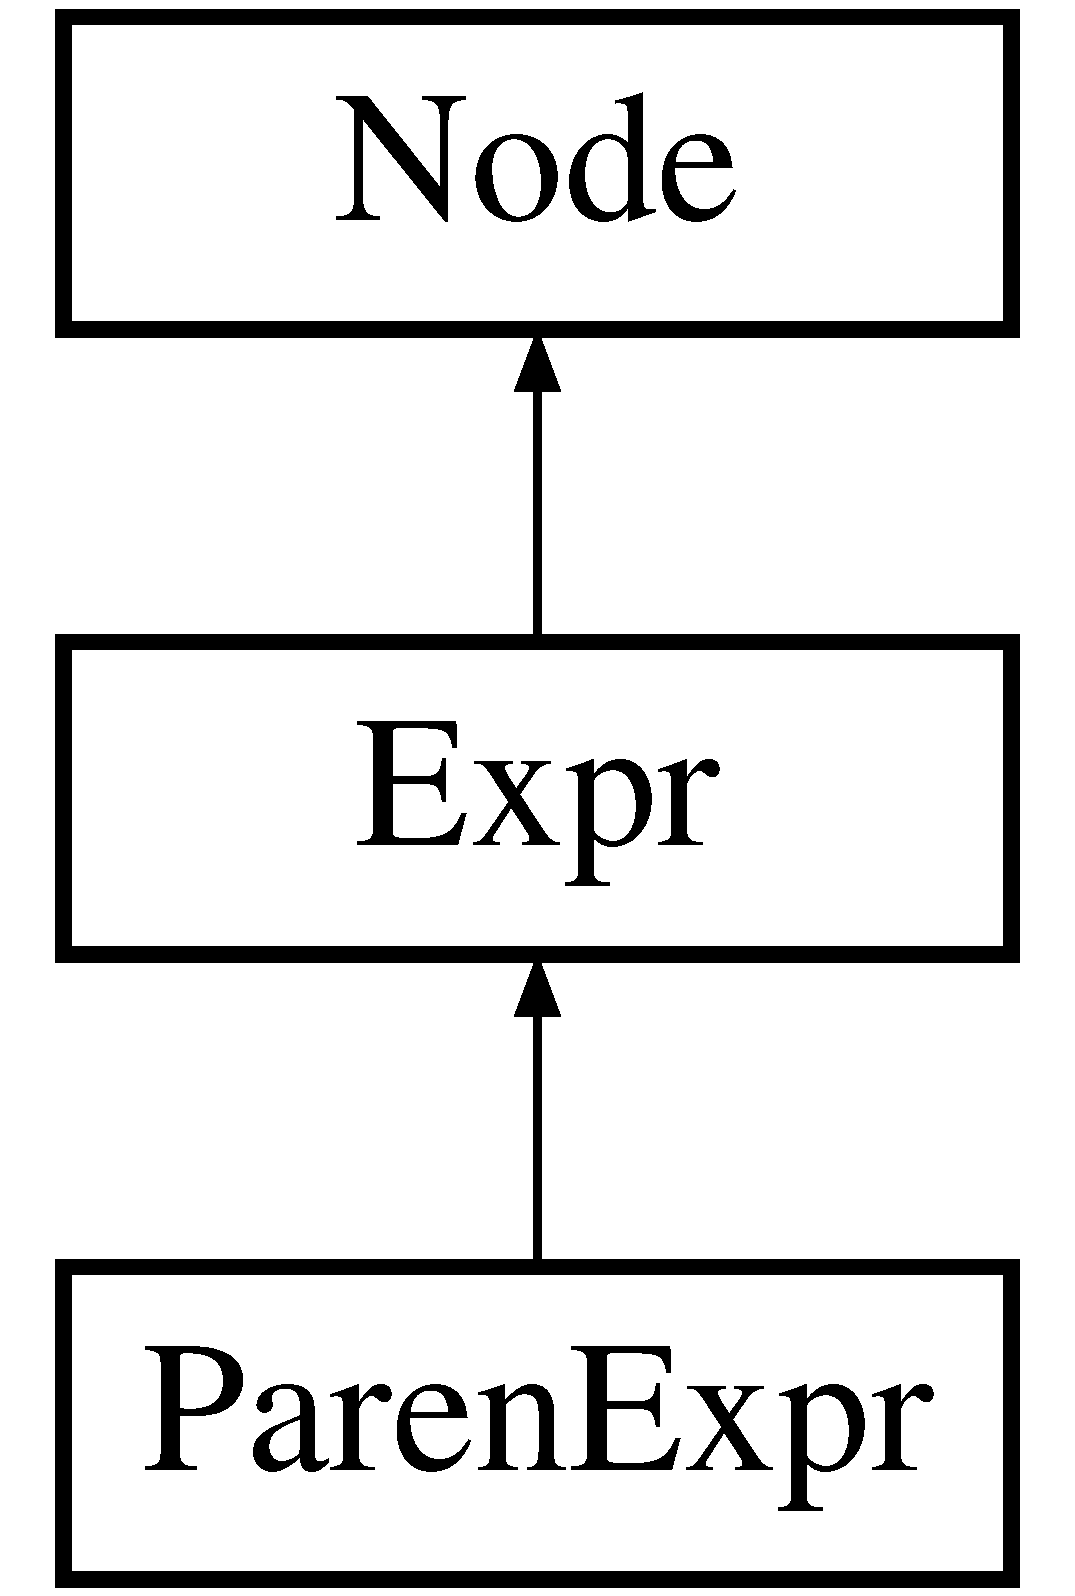
\includegraphics[height=3.000000cm]{classParenExpr}
\end{center}
\end{figure}
\subsection*{Public Member Functions}
\begin{DoxyCompactItemize}
\item 
\hypertarget{classParenExpr_ad3b11932be46c6b7af4a71c4265cfa75}{{\bfseries Paren\-Expr} (\hyperlink{classExpr}{Expr} $\ast$e)}\label{classParenExpr_ad3b11932be46c6b7af4a71c4265cfa75}

\item 
\hypertarget{classParenExpr_a894bdf8546f0242c85b4664a2f9492cd}{std\-::string \hyperlink{classParenExpr_a894bdf8546f0242c85b4664a2f9492cd}{unparse} ()}\label{classParenExpr_a894bdf8546f0242c85b4664a2f9492cd}

\begin{DoxyCompactList}\small\item\em Unparse the paren brackets and expression (recursively) within. \end{DoxyCompactList}\end{DoxyCompactItemize}


\subsection{Detailed Description}
\hyperlink{classExpr}{Expr} \-:\-:= '(' \hyperlink{classExpr}{Expr} ')'. 

The documentation for this class was generated from the following file\-:\begin{DoxyCompactItemize}
\item 
A\-S\-T.\-h\end{DoxyCompactItemize}

\hypertarget{classParser}{\section{Parser Class Reference}
\label{classParser}\index{Parser@{Parser}}
}
\subsection*{Public Member Functions}
\begin{DoxyCompactItemize}
\item 
\hypertarget{classParser_a12234f6cd36b61af4b50c94a179422c1}{\hyperlink{classParser_a12234f6cd36b61af4b50c94a179422c1}{Parser} ()}\label{classParser_a12234f6cd36b61af4b50c94a179422c1}

\begin{DoxyCompactList}\small\item\em \hyperlink{classParser}{Parser} constructor initializes all nodes of the A\-S\-T to N\-U\-L\-L. \end{DoxyCompactList}\item 
\hypertarget{classParser_a3e658b5917a93a3ef648050d060e3a93}{\hyperlink{classParser_a3e658b5917a93a3ef648050d060e3a93}{$\sim$\-Parser} ()}\label{classParser_a3e658b5917a93a3ef648050d060e3a93}

\begin{DoxyCompactList}\small\item\em \hyperlink{classParser}{Parser} destructor, uses 'delete' to free memory dynamically located on the heap. \end{DoxyCompactList}\item 
\hyperlink{classParseResult}{Parse\-Result} \hyperlink{classParser_a2c1a7aa0b09a43bc1eef460817efb1d6}{parse} (const char $\ast$text)
\begin{DoxyCompactList}\small\item\em parse takes in a char $\ast$text dsl program and returns the parsed result \end{DoxyCompactList}\item 
\hyperlink{classParseResult}{Parse\-Result} \hyperlink{classParser_a14e25c84322809e2f060dc530362ea71}{parse\-Program} ()
\item 
\hyperlink{classParseResult}{Parse\-Result} \hyperlink{classParser_ac646227983887c1cd13dae67fa1bc142}{parse\-Decl} ()
\item 
\hyperlink{classParseResult}{Parse\-Result} \hyperlink{classParser_a1e1f83c0f4b11148a356d951f191425e}{parse\-Standard\-Decl} ()
\item 
\hyperlink{classParseResult}{Parse\-Result} \hyperlink{classParser_a3a00df25fda2af308b69f05eed14ac69}{parse\-Matrix\-Decl} ()
\item 
\hyperlink{classParseResult}{Parse\-Result} \hyperlink{classParser_a452db3def31683cb0305e57a01489bd4}{parse\-Stmts} ()
\begin{DoxyCompactList}\small\item\em parse\-Stmts results in either a new 'stmt \hyperlink{classStmts}{Stmts}' or 'empty\-Stmts' (grammar lines 2 or 3) \end{DoxyCompactList}\item 
\hyperlink{classParseResult}{Parse\-Result} \hyperlink{classParser_a9709c4793d0cce012d595f3ee416cd25}{parse\-Stmt} ()
\begin{DoxyCompactList}\small\item\em \hyperlink{classStmt}{Stmt}. \end{DoxyCompactList}\item 
\hyperlink{classParseResult}{Parse\-Result} \hyperlink{classParser_a50227dc24dc7a175ac0533d9957dfcf8}{parse\-Expr} (int rbp)
\begin{DoxyCompactList}\small\item\em \hyperlink{classExpr}{Expr}. \end{DoxyCompactList}\item 
\hyperlink{classParseResult}{Parse\-Result} \hyperlink{classParser_ad40f1e5e4c66814f959d982f94b767a3}{parse\-True\-Kwd} ()
\begin{DoxyCompactList}\small\item\em \hyperlink{classExpr}{Expr} \-:\-:= true\-Kwd. \end{DoxyCompactList}\item 
\hypertarget{classParser_a56f03d2e70d12648c55ce56a11e63324}{\hyperlink{classParseResult}{Parse\-Result} \hyperlink{classParser_a56f03d2e70d12648c55ce56a11e63324}{parse\-False\-Kwd} ()}\label{classParser_a56f03d2e70d12648c55ce56a11e63324}

\begin{DoxyCompactList}\small\item\em \hyperlink{classExpr}{Expr} \-:\-:= false\-Kwd. \end{DoxyCompactList}\item 
\hypertarget{classParser_a2b200b744e5bedf82ef6f610d7877cfc}{\hyperlink{classParseResult}{Parse\-Result} \hyperlink{classParser_a2b200b744e5bedf82ef6f610d7877cfc}{parse\-Int\-Const} ()}\label{classParser_a2b200b744e5bedf82ef6f610d7877cfc}

\begin{DoxyCompactList}\small\item\em \hyperlink{classExpr}{Expr} \-:\-:= int\-Const. \end{DoxyCompactList}\item 
\hypertarget{classParser_aaf7b1176fd53246f59577c7eec8b9d22}{\hyperlink{classParseResult}{Parse\-Result} \hyperlink{classParser_aaf7b1176fd53246f59577c7eec8b9d22}{parse\-Float\-Const} ()}\label{classParser_aaf7b1176fd53246f59577c7eec8b9d22}

\begin{DoxyCompactList}\small\item\em \hyperlink{classExpr}{Expr} \-:\-:= float\-Const. \end{DoxyCompactList}\item 
\hypertarget{classParser_a4d8930d45c2b730912154c46cc54833c}{\hyperlink{classParseResult}{Parse\-Result} \hyperlink{classParser_a4d8930d45c2b730912154c46cc54833c}{parse\-String\-Const} ()}\label{classParser_a4d8930d45c2b730912154c46cc54833c}

\begin{DoxyCompactList}\small\item\em \hyperlink{classExpr}{Expr} \-:\-:= string\-Const. \end{DoxyCompactList}\item 
\hypertarget{classParser_a49c9b3d31ca060c97873e5485d518da3}{\hyperlink{classParseResult}{Parse\-Result} {\bfseries parse\-Char\-Const} ()}\label{classParser_a49c9b3d31ca060c97873e5485d518da3}

\item 
\hyperlink{classParseResult}{Parse\-Result} \hyperlink{classParser_a8c1baf62f71da64590e883e51ce622ca}{parse\-Variable\-Name} ()
\begin{DoxyCompactList}\small\item\em \hyperlink{classExpr}{Expr} \-:\-:= variable\-Name ..... \end{DoxyCompactList}\item 
\hypertarget{classParser_aec4c38e1e63c9becfd3a8fc4a1a73f01}{\hyperlink{classParseResult}{Parse\-Result} \hyperlink{classParser_aec4c38e1e63c9becfd3a8fc4a1a73f01}{parse\-Nested\-Expr} ()}\label{classParser_aec4c38e1e63c9becfd3a8fc4a1a73f01}

\begin{DoxyCompactList}\small\item\em \hyperlink{classExpr}{Expr} \-:\-:= '(' \hyperlink{classExpr}{Expr} ')'. \end{DoxyCompactList}\item 
\hypertarget{classParser_a1503ceff46112d6d4f0e01b5fb77afcd}{\hyperlink{classParseResult}{Parse\-Result} \hyperlink{classParser_a1503ceff46112d6d4f0e01b5fb77afcd}{parse\-Not\-Expr} ()}\label{classParser_a1503ceff46112d6d4f0e01b5fb77afcd}

\begin{DoxyCompactList}\small\item\em \hyperlink{classExpr}{Expr} \-:\-:= '!' \hyperlink{classExpr}{Expr}. \end{DoxyCompactList}\item 
\hypertarget{classParser_aa24c33b04779801b330d7fe5a74349e5}{\hyperlink{classParseResult}{Parse\-Result} \hyperlink{classParser_aa24c33b04779801b330d7fe5a74349e5}{parse\-Let\-Expr} ()}\label{classParser_aa24c33b04779801b330d7fe5a74349e5}

\begin{DoxyCompactList}\small\item\em \hyperlink{classExpr}{Expr} \-:\-:= 'let' \hyperlink{classStmts}{Stmts} 'in' \hyperlink{classExpr}{Expr} 'end'. \end{DoxyCompactList}\item 
\hypertarget{classParser_a555bc6f671d408208e6d049f8e9f3c86}{\hyperlink{classParseResult}{Parse\-Result} \hyperlink{classParser_a555bc6f671d408208e6d049f8e9f3c86}{parse\-If\-Expr} ()}\label{classParser_a555bc6f671d408208e6d049f8e9f3c86}

\begin{DoxyCompactList}\small\item\em \hyperlink{classExpr}{Expr} \-:\-:= 'if' \hyperlink{classExpr}{Expr} 'then' \hyperlink{classExpr}{Expr} 'else' \hyperlink{classExpr}{Expr}. \end{DoxyCompactList}\item 
\hyperlink{classParseResult}{Parse\-Result} \hyperlink{classParser_ae09cb2b5a7f80c6ad4ad9ccf27a746ca}{parse\-Addition} (\hyperlink{classParseResult}{Parse\-Result} left)
\begin{DoxyCompactList}\small\item\em \hyperlink{classExpr}{Expr} \-:\-:= \hyperlink{classExpr}{Expr} '+' \hyperlink{classExpr}{Expr}. \end{DoxyCompactList}\item 
\hyperlink{classParseResult}{Parse\-Result} \hyperlink{classParser_a52e6a57d53fc98e5819cc51b3cbe5bd5}{parse\-Multiplication} (\hyperlink{classParseResult}{Parse\-Result} left)
\begin{DoxyCompactList}\small\item\em \hyperlink{classExpr}{Expr} \-:\-:= \hyperlink{classExpr}{Expr} '$\ast$' \hyperlink{classExpr}{Expr}. \end{DoxyCompactList}\item 
\hyperlink{classParseResult}{Parse\-Result} \hyperlink{classParser_ac22cf1f77e0ca4c23942d5cbcc47eb37}{parse\-Subtraction} (\hyperlink{classParseResult}{Parse\-Result} left)
\begin{DoxyCompactList}\small\item\em \hyperlink{classExpr}{Expr} \-:\-:= \hyperlink{classExpr}{Expr} '-\/' \hyperlink{classExpr}{Expr}. \end{DoxyCompactList}\item 
\hyperlink{classParseResult}{Parse\-Result} \hyperlink{classParser_ad05e6cd1bf83179ecb727b83cbbd0c4e}{parse\-Division} (\hyperlink{classParseResult}{Parse\-Result} left)
\begin{DoxyCompactList}\small\item\em \hyperlink{classExpr}{Expr} \-:\-:= \hyperlink{classExpr}{Expr} '/' \hyperlink{classExpr}{Expr}. \end{DoxyCompactList}\item 
\hyperlink{classParseResult}{Parse\-Result} \hyperlink{classParser_ab42ecabc4dbe601d5ed9667351c0c0b8}{parse\-Relational\-Expr} (\hyperlink{classParseResult}{Parse\-Result} left)
\item 
\hypertarget{classParser_a3199aab5275c8b6477245eb866fabf35}{void \hyperlink{classParser_a3199aab5275c8b6477245eb866fabf35}{match} (token\-Type tt)}\label{classParser_a3199aab5275c8b6477245eb866fabf35}

\begin{DoxyCompactList}\small\item\em Helper function used by the parser. \end{DoxyCompactList}\item 
\hypertarget{classParser_a151ffb920a67527813d77bc4ba44c4a7}{bool \hyperlink{classParser_a151ffb920a67527813d77bc4ba44c4a7}{attempt\-Match} (token\-Type tt)}\label{classParser_a151ffb920a67527813d77bc4ba44c4a7}

\begin{DoxyCompactList}\small\item\em Verify that the token matches, if so, advance to the next token. \end{DoxyCompactList}\item 
\hypertarget{classParser_a67a10b685bd263477b5f59f1923cdec3}{bool {\bfseries next\-Is} (token\-Type tt)}\label{classParser_a67a10b685bd263477b5f59f1923cdec3}

\item 
\hypertarget{classParser_a324a5bb61c9dfc645300a92aecd6fe69}{void \hyperlink{classParser_a324a5bb61c9dfc645300a92aecd6fe69}{next\-Token} ()}\label{classParser_a324a5bb61c9dfc645300a92aecd6fe69}

\begin{DoxyCompactList}\small\item\em Advance prev\-Token and curr\-Token if no errors are found. \end{DoxyCompactList}\item 
\hypertarget{classParser_a1f45059a13bc0c98355278a9ca9feed9}{std\-::string {\bfseries terminal\-Description} (token\-Type terminal)}\label{classParser_a1f45059a13bc0c98355278a9ca9feed9}

\item 
\hypertarget{classParser_a341bee73e8b1e8558505a237846b16b3}{std\-::string {\bfseries make\-Error\-Msg} (token\-Type terminal)}\label{classParser_a341bee73e8b1e8558505a237846b16b3}

\item 
\hypertarget{classParser_ad38e58ddee85db2aecbd3c7bdcf42116}{std\-::string {\bfseries make\-Error\-Msg\-Expected} (token\-Type terminal)}\label{classParser_ad38e58ddee85db2aecbd3c7bdcf42116}

\item 
\hypertarget{classParser_a60c23daeffb7ced92599e4f2555f71c9}{std\-::string {\bfseries make\-Error\-Msg} (const char $\ast$msg)}\label{classParser_a60c23daeffb7ced92599e4f2555f71c9}

\end{DoxyCompactItemize}
\subsection*{Public Attributes}
\begin{DoxyCompactItemize}
\item 
\hypertarget{classParser_a3606ff327be18af7f76df95f50851633}{\hyperlink{classExtToken}{Ext\-Token} $\ast$ {\bfseries tokens}}\label{classParser_a3606ff327be18af7f76df95f50851633}

\item 
\hypertarget{classParser_a75ab2e2b9385c14e5f967f873340ed11}{\hyperlink{classExtToken}{Ext\-Token} $\ast$ {\bfseries curr\-Token}}\label{classParser_a75ab2e2b9385c14e5f967f873340ed11}

\item 
\hypertarget{classParser_a4bcf7560a5ea1b486bbe4bb54a5a22eb}{\hyperlink{classExtToken}{Ext\-Token} $\ast$ {\bfseries prev\-Token}}\label{classParser_a4bcf7560a5ea1b486bbe4bb54a5a22eb}

\item 
\hypertarget{classParser_a0910de176dcc1cdfbf7ad99622ce9dd5}{\hyperlink{classToken}{Token} $\ast$ {\bfseries stokens}}\label{classParser_a0910de176dcc1cdfbf7ad99622ce9dd5}

\item 
\hypertarget{classParser_ab2ef99ea9e732f5fd176b3949a6c32af}{\hyperlink{classScanner}{Scanner} $\ast$ {\bfseries s}}\label{classParser_ab2ef99ea9e732f5fd176b3949a6c32af}

\end{DoxyCompactItemize}


\subsection{Member Function Documentation}
\hypertarget{classParser_a2c1a7aa0b09a43bc1eef460817efb1d6}{\index{Parser@{Parser}!parse@{parse}}
\index{parse@{parse}!Parser@{Parser}}
\subsubsection[{parse}]{\setlength{\rightskip}{0pt plus 5cm}{\bf Parse\-Result} Parser\-::parse (
\begin{DoxyParamCaption}
\item[{const char $\ast$}]{text}
\end{DoxyParamCaption}
)}}\label{classParser_a2c1a7aa0b09a43bc1eef460817efb1d6}


parse takes in a char $\ast$text dsl program and returns the parsed result 

This is the catch for condition 2 in \hyperlink{ast__tests_8h_source}{ast\-\_\-tests.\-h} \hypertarget{classParser_ae09cb2b5a7f80c6ad4ad9ccf27a746ca}{\index{Parser@{Parser}!parse\-Addition@{parse\-Addition}}
\index{parse\-Addition@{parse\-Addition}!Parser@{Parser}}
\subsubsection[{parse\-Addition}]{\setlength{\rightskip}{0pt plus 5cm}{\bf Parse\-Result} Parser\-::parse\-Addition (
\begin{DoxyParamCaption}
\item[{{\bf Parse\-Result}}]{left}
\end{DoxyParamCaption}
)}}\label{classParser_ae09cb2b5a7f80c6ad4ad9ccf27a746ca}


\hyperlink{classExpr}{Expr} \-:\-:= \hyperlink{classExpr}{Expr} '+' \hyperlink{classExpr}{Expr}. 

parser has already matched left expression

Create the node for the left expression

Create the node and set up the right expression \hypertarget{classParser_ac646227983887c1cd13dae67fa1bc142}{\index{Parser@{Parser}!parse\-Decl@{parse\-Decl}}
\index{parse\-Decl@{parse\-Decl}!Parser@{Parser}}
\subsubsection[{parse\-Decl}]{\setlength{\rightskip}{0pt plus 5cm}{\bf Parse\-Result} Parser\-::parse\-Decl (
\begin{DoxyParamCaption}
{}
\end{DoxyParamCaption}
)}}\label{classParser_ac646227983887c1cd13dae67fa1bc142}
\hyperlink{classDecl}{Decl} Determines whether to parse a standard declaration or a matrix declaration \hyperlink{classDecl}{Decl} \-:\-: Matrix variable\-Name ....

\hyperlink{classDecl}{Decl} \-:\-:= Type variable\-Name semi\-Colon \hypertarget{classParser_ad05e6cd1bf83179ecb727b83cbbd0c4e}{\index{Parser@{Parser}!parse\-Division@{parse\-Division}}
\index{parse\-Division@{parse\-Division}!Parser@{Parser}}
\subsubsection[{parse\-Division}]{\setlength{\rightskip}{0pt plus 5cm}{\bf Parse\-Result} Parser\-::parse\-Division (
\begin{DoxyParamCaption}
\item[{{\bf Parse\-Result}}]{left}
\end{DoxyParamCaption}
)}}\label{classParser_ad05e6cd1bf83179ecb727b83cbbd0c4e}


\hyperlink{classExpr}{Expr} \-:\-:= \hyperlink{classExpr}{Expr} '/' \hyperlink{classExpr}{Expr}. 

parser has already matched left expression

Create the node for the left expression

Create the node and set up the right expression \hypertarget{classParser_a50227dc24dc7a175ac0533d9957dfcf8}{\index{Parser@{Parser}!parse\-Expr@{parse\-Expr}}
\index{parse\-Expr@{parse\-Expr}!Parser@{Parser}}
\subsubsection[{parse\-Expr}]{\setlength{\rightskip}{0pt plus 5cm}{\bf Parse\-Result} Parser\-::parse\-Expr (
\begin{DoxyParamCaption}
\item[{int}]{rbp}
\end{DoxyParamCaption}
)}}\label{classParser_a50227dc24dc7a175ac0533d9957dfcf8}


\hyperlink{classExpr}{Expr}. 

Examine current token, without consuming it, to call its associated parse methods. The \hyperlink{classExtToken}{Ext\-Token} objects have 'nud' and 'led' methods that are dispatchers that call the appropriate parse methods.\hypertarget{classParser_a3a00df25fda2af308b69f05eed14ac69}{\index{Parser@{Parser}!parse\-Matrix\-Decl@{parse\-Matrix\-Decl}}
\index{parse\-Matrix\-Decl@{parse\-Matrix\-Decl}!Parser@{Parser}}
\subsubsection[{parse\-Matrix\-Decl}]{\setlength{\rightskip}{0pt plus 5cm}{\bf Parse\-Result} Parser\-::parse\-Matrix\-Decl (
\begin{DoxyParamCaption}
{}
\end{DoxyParamCaption}
)}}\label{classParser_a3a00df25fda2af308b69f05eed14ac69}
Matrix\-Decl Identical purpose of parse\-Decl, handles special matrix syntax. \hyperlink{classDecl}{Decl} \-:\-:= 'matrix' var\-Name '\mbox{[}' \hyperlink{classExpr}{Expr} '\-:' \hyperlink{classExpr}{Expr} '\mbox{]}' var\-Name '\-:' var\-Name '=' \hyperlink{classExpr}{Expr} ';'

\hyperlink{classDecl}{Decl} \-:\-:= 'matrix' var\-Name '=' \hyperlink{classExpr}{Expr} ';' \hypertarget{classParser_a52e6a57d53fc98e5819cc51b3cbe5bd5}{\index{Parser@{Parser}!parse\-Multiplication@{parse\-Multiplication}}
\index{parse\-Multiplication@{parse\-Multiplication}!Parser@{Parser}}
\subsubsection[{parse\-Multiplication}]{\setlength{\rightskip}{0pt plus 5cm}{\bf Parse\-Result} Parser\-::parse\-Multiplication (
\begin{DoxyParamCaption}
\item[{{\bf Parse\-Result}}]{left}
\end{DoxyParamCaption}
)}}\label{classParser_a52e6a57d53fc98e5819cc51b3cbe5bd5}


\hyperlink{classExpr}{Expr} \-:\-:= \hyperlink{classExpr}{Expr} '$\ast$' \hyperlink{classExpr}{Expr}. 

parser has already matched left expression

Create the node for the left expression

Create the node and set up the right expression \hypertarget{classParser_a14e25c84322809e2f060dc530362ea71}{\index{Parser@{Parser}!parse\-Program@{parse\-Program}}
\index{parse\-Program@{parse\-Program}!Parser@{Parser}}
\subsubsection[{parse\-Program}]{\setlength{\rightskip}{0pt plus 5cm}{\bf Parse\-Result} Parser\-::parse\-Program (
\begin{DoxyParamCaption}
{}
\end{DoxyParamCaption}
)}}\label{classParser_a14e25c84322809e2f060dc530362ea71}
\subsubsection*{parse methods for non-\/terminal symbols }

parse\-Program is used to fully parse grammar line 1 and recursively build the abstract syntax tree (ast) root \hyperlink{classProgram}{Program} \-:\-:= var\-Name '(' ')' '\{' \hyperlink{classStmts}{Stmts} '\}' Match helper function, throws exception if token doesn't match, moves to next token if match is true

Direct initialization. The string variable 'name' is initialized to the lexeme of the dereferenced pointer 'prev\-Token'

Initialize varname from grammar line 1 (i.\-e. \char`\"{}main\char`\"{})

Create \hyperlink{classStmt}{Stmt} \hyperlink{classStmts}{Stmts} nodes

Create a stmts root node for all the nodes recursively created through pr\-Stmts above

ast is a \hyperlink{classNode}{Node} pointer found in \hyperlink{parseResult_8h_source}{parse\-Result.\-h}

Fully parsed program to be returned \hypertarget{classParser_ab42ecabc4dbe601d5ed9667351c0c0b8}{\index{Parser@{Parser}!parse\-Relational\-Expr@{parse\-Relational\-Expr}}
\index{parse\-Relational\-Expr@{parse\-Relational\-Expr}!Parser@{Parser}}
\subsubsection[{parse\-Relational\-Expr}]{\setlength{\rightskip}{0pt plus 5cm}{\bf Parse\-Result} Parser\-::parse\-Relational\-Expr (
\begin{DoxyParamCaption}
\item[{{\bf Parse\-Result}}]{pr\-Left}
\end{DoxyParamCaption}
)}}\label{classParser_ab42ecabc4dbe601d5ed9667351c0c0b8}
\hyperlink{classExpr}{Expr} \-:\-:= \hyperlink{classExpr}{Expr} equal\-Equals \hyperlink{classExpr}{Expr} \hyperlink{classExpr}{Expr} \-:\-:= \hyperlink{classExpr}{Expr} less\-Than\-Equals \hyperlink{classExpr}{Expr} \hyperlink{classExpr}{Expr} \-:\-:= \hyperlink{classExpr}{Expr} greater\-Than\-Equals \hyperlink{classExpr}{Expr} \hyperlink{classExpr}{Expr} \-:\-:= \hyperlink{classExpr}{Expr} not\-Equals \hyperlink{classExpr}{Expr} \hyperlink{classExpr}{Expr} \-:\-:= \hyperlink{classExpr}{Expr} left\-Angle \hyperlink{classExpr}{Expr} \hyperlink{classExpr}{Expr} \-:\-:= \hyperlink{classExpr}{Expr} right\-Angle \hyperlink{classExpr}{Expr}

Notice that for relational operators we use just one parse function. This shows another possible means for implementing expressions, as opposed to the method used for arithmetic expressions in which each operation has its own parse method. It will depend on what we do in iteration 3 in building an abstract syntax tree to decide which method is better. parser has already matched left expression

Create the node for the left expression

just advance token, since examining it in parse\-Expr caused this method being called.

Create the node and set up the right expression \hypertarget{classParser_a1e1f83c0f4b11148a356d951f191425e}{\index{Parser@{Parser}!parse\-Standard\-Decl@{parse\-Standard\-Decl}}
\index{parse\-Standard\-Decl@{parse\-Standard\-Decl}!Parser@{Parser}}
\subsubsection[{parse\-Standard\-Decl}]{\setlength{\rightskip}{0pt plus 5cm}{\bf Parse\-Result} Parser\-::parse\-Standard\-Decl (
\begin{DoxyParamCaption}
{}
\end{DoxyParamCaption}
)}}\label{classParser_a1e1f83c0f4b11148a356d951f191425e}
standard\-Decl \hyperlink{classDecl}{Decl} \-:\-:= integer\-Kwd var\-Name $\vert$ float\-Kwd var\-Name $\vert$ string\-Kwd var\-Name $\vert$ bool\-Kwd var\-Name \hyperlink{classParseResult}{Parse\-Result} pr\-Type = parse\-Type() ;

Type \-:\-:= int\-Kwd

Type \-:\-:= float\-Kwd

Type \-:\-:= string\-Kwd

Type \-:\-:= bool\-Kwd

From the current standard declaration, parse the variable name (as a string)

Create the new standard declaration with the keyword type and variable name \hypertarget{classParser_a9709c4793d0cce012d595f3ee416cd25}{\index{Parser@{Parser}!parse\-Stmt@{parse\-Stmt}}
\index{parse\-Stmt@{parse\-Stmt}!Parser@{Parser}}
\subsubsection[{parse\-Stmt}]{\setlength{\rightskip}{0pt plus 5cm}{\bf Parse\-Result} Parser\-::parse\-Stmt (
\begin{DoxyParamCaption}
{}
\end{DoxyParamCaption}
)}}\label{classParser_a9709c4793d0cce012d595f3ee416cd25}


\hyperlink{classStmt}{Stmt}. 

\hyperlink{classStmt}{Stmt} \-:\-:= \hyperlink{classDecl}{Decl}

\hyperlink{classStmt}{Stmt} \-:\-:= '\{' \hyperlink{classStmts}{Stmts} '\}'

\hyperlink{classStmt}{Stmt} \-:\-:= 'if' '(' \hyperlink{classExpr}{Expr} ')' \hyperlink{classStmt}{Stmt} \hyperlink{classStmt}{Stmt} \-:\-:= 'if' '(' \hyperlink{classExpr}{Expr} ')' \hyperlink{classStmt}{Stmt} 'else' \hyperlink{classStmt}{Stmt}

Handle if/else statement

Handle only if statement

\hyperlink{classStmt}{Stmt} \-:\-:= var\-Name '=' \hyperlink{classExpr}{Expr} ';' $\vert$ var\-Name '\mbox{[}' \hyperlink{classExpr}{Expr} '\-:' \hyperlink{classExpr}{Expr} '\mbox{]}' '=' \hyperlink{classExpr}{Expr} ';'

Determine whether it's a regular assignment or matrix assignment

Parse the first matrix expression

Parse the second matrix expression

ast is the pointer to the \hyperlink{classNode}{Node} of pr\-Expr (\hyperlink{classParseResult}{Parse\-Result})

Handle matrix assignment statement

Handle regular assignment statement

\hyperlink{classStmt}{Stmt} \-:\-:= 'print' '(' \hyperlink{classExpr}{Expr} ')' ';'

\hyperlink{classStmt}{Stmt} \-:\-:= 'repeat' '(' var\-Name '=' \hyperlink{classExpr}{Expr} 'to' \hyperlink{classExpr}{Expr} ')' \hyperlink{classStmt}{Stmt}

\hyperlink{classStmt}{Stmt} \-:\-:= 'while' '(' \hyperlink{classExpr}{Expr} ')' \hyperlink{classStmt}{Stmt}

\hyperlink{classStmt}{Stmt} \-:\-:= ';

parsed a skip

\hyperlink{classStmt}{Stmt} \-:\-:= variable\-Name assign \hyperlink{classExpr}{Expr} semi\-Colon \hypertarget{classParser_a452db3def31683cb0305e57a01489bd4}{\index{Parser@{Parser}!parse\-Stmts@{parse\-Stmts}}
\index{parse\-Stmts@{parse\-Stmts}!Parser@{Parser}}
\subsubsection[{parse\-Stmts}]{\setlength{\rightskip}{0pt plus 5cm}{\bf Parse\-Result} Parser\-::parse\-Stmts (
\begin{DoxyParamCaption}
{}
\end{DoxyParamCaption}
)}}\label{classParser_a452db3def31683cb0305e57a01489bd4}


parse\-Stmts results in either a new 'stmt \hyperlink{classStmts}{Stmts}' or 'empty\-Stmts' (grammar lines 2 or 3) 

\hyperlink{classStmts}{Stmts} \-:\-:= \hyperlink{classStmt}{Stmt} \hyperlink{classStmts}{Stmts}

\hyperlink{classNode}{Node} for \hyperlink{classStmt}{Stmt}

\hyperlink{classNode}{Node} for \hyperlink{classStmts}{Stmts}; recurse this function

Create stmt\-Stmts junction, the stmt\-Stmts constructor expects pointers for the

\hyperlink{classStmt}{Stmt} and \hyperlink{classStmts}{Stmts} nodes

\hyperlink{classStmts}{Stmts} \-:\-:= nothing to match. \hypertarget{classParser_ac22cf1f77e0ca4c23942d5cbcc47eb37}{\index{Parser@{Parser}!parse\-Subtraction@{parse\-Subtraction}}
\index{parse\-Subtraction@{parse\-Subtraction}!Parser@{Parser}}
\subsubsection[{parse\-Subtraction}]{\setlength{\rightskip}{0pt plus 5cm}{\bf Parse\-Result} Parser\-::parse\-Subtraction (
\begin{DoxyParamCaption}
\item[{{\bf Parse\-Result}}]{left}
\end{DoxyParamCaption}
)}}\label{classParser_ac22cf1f77e0ca4c23942d5cbcc47eb37}


\hyperlink{classExpr}{Expr} \-:\-:= \hyperlink{classExpr}{Expr} '-\/' \hyperlink{classExpr}{Expr}. 

parser has already matched left expression

Create the node for the left expression

Create the node and set up the right expression \hypertarget{classParser_ad40f1e5e4c66814f959d982f94b767a3}{\index{Parser@{Parser}!parse\-True\-Kwd@{parse\-True\-Kwd}}
\index{parse\-True\-Kwd@{parse\-True\-Kwd}!Parser@{Parser}}
\subsubsection[{parse\-True\-Kwd}]{\setlength{\rightskip}{0pt plus 5cm}{\bf Parse\-Result} Parser\-::parse\-True\-Kwd (
\begin{DoxyParamCaption}
{}
\end{DoxyParamCaption}
)}}\label{classParser_ad40f1e5e4c66814f959d982f94b767a3}


\hyperlink{classExpr}{Expr} \-:\-:= true\-Kwd. 

\subsubsection*{parse methods for \hyperlink{classExpr}{Expr} productions }\hypertarget{classParser_a8c1baf62f71da64590e883e51ce622ca}{\index{Parser@{Parser}!parse\-Variable\-Name@{parse\-Variable\-Name}}
\index{parse\-Variable\-Name@{parse\-Variable\-Name}!Parser@{Parser}}
\subsubsection[{parse\-Variable\-Name}]{\setlength{\rightskip}{0pt plus 5cm}{\bf Parse\-Result} Parser\-::parse\-Variable\-Name (
\begin{DoxyParamCaption}
{}
\end{DoxyParamCaption}
)}}\label{classParser_a8c1baf62f71da64590e883e51ce622ca}


\hyperlink{classExpr}{Expr} \-:\-:= variable\-Name ..... 

\hyperlink{classExpr}{Expr} \-:\-:= variable\-Name '\mbox{[}' \hyperlink{classExpr}{Expr} '\-:' \hyperlink{classExpr}{Expr} '\mbox{]}' \hyperlink{classMatrixRef}{Matrix\-Ref}

\hyperlink{classExpr}{Expr} \-:\-:= varable\-Name '(' \hyperlink{classExpr}{Expr} ')' Nested\-Or\-Function\-Call

\hyperlink{classExpr}{Expr} \-:= variable\-Name

variable 

The documentation for this class was generated from the following files\-:\begin{DoxyCompactItemize}
\item 
parser.\-h\item 
parser.\-cpp\end{DoxyCompactItemize}

\hypertarget{classParseResult}{\section{Parse\-Result Class Reference}
\label{classParseResult}\index{Parse\-Result@{Parse\-Result}}
}
\subsection*{Public Attributes}
\begin{DoxyCompactItemize}
\item 
\hypertarget{classParseResult_ab2dd8deb95c5177148f488ca5d31307a}{std\-::string {\bfseries errors}}\label{classParseResult_ab2dd8deb95c5177148f488ca5d31307a}

\item 
\hypertarget{classParseResult_aa04c6ed3cba109f276e5bc089ca2ff15}{\hyperlink{classNode}{Node} $\ast$ {\bfseries ast}}\label{classParseResult_aa04c6ed3cba109f276e5bc089ca2ff15}

\item 
\hypertarget{classParseResult_a64eb6658c1fc5bbf35fdce181f6845d5}{bool {\bfseries ok}}\label{classParseResult_a64eb6658c1fc5bbf35fdce181f6845d5}

\end{DoxyCompactItemize}


The documentation for this class was generated from the following files\-:\begin{DoxyCompactItemize}
\item 
parse\-Result.\-h\item 
parse\-Result.\-cpp\end{DoxyCompactItemize}

\hypertarget{classParserTestSuite}{\section{Parser\-Test\-Suite Class Reference}
\label{classParserTestSuite}\index{Parser\-Test\-Suite@{Parser\-Test\-Suite}}
}
Inheritance diagram for Parser\-Test\-Suite\-:\begin{figure}[H]
\begin{center}
\leavevmode
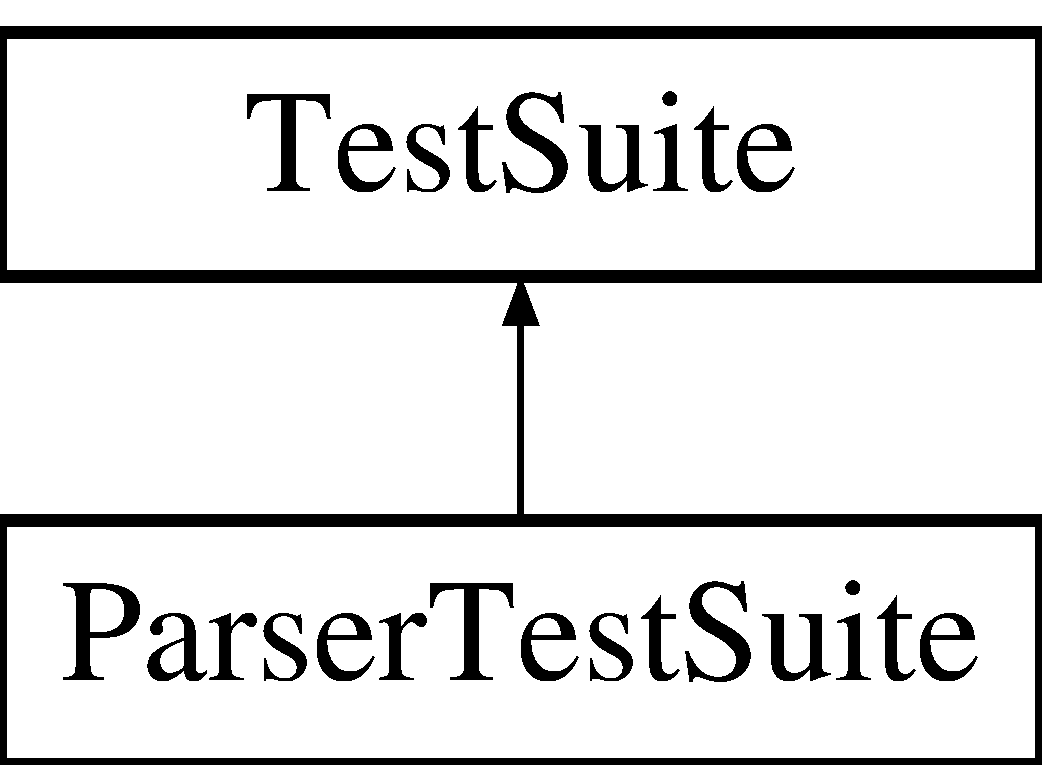
\includegraphics[height=2.000000cm]{classParserTestSuite}
\end{center}
\end{figure}
\subsection*{Public Member Functions}
\begin{DoxyCompactItemize}
\item 
\hypertarget{classParserTestSuite_ab7eff3217b5e28c9003f27c51da107ac}{void {\bfseries test\-\_\-setup\-\_\-code} ()}\label{classParserTestSuite_ab7eff3217b5e28c9003f27c51da107ac}

\item 
\hypertarget{classParserTestSuite_ac4a829a66a1582bee38e90ac3f0355f4}{void {\bfseries test\-\_\-parse\-\_\-bad\-\_\-syntax} ()}\label{classParserTestSuite_ac4a829a66a1582bee38e90ac3f0355f4}

\item 
\hypertarget{classParserTestSuite_a26eed485bc2671f4ac256ef97a21b704}{void {\bfseries test\-\_\-parse\-\_\-sample\-\_\-1} ()}\label{classParserTestSuite_a26eed485bc2671f4ac256ef97a21b704}

\item 
\hypertarget{classParserTestSuite_a0f1d6af1e07e35541fb83416d5e3e229}{void {\bfseries test\-\_\-parse\-\_\-sample\-\_\-2} ()}\label{classParserTestSuite_a0f1d6af1e07e35541fb83416d5e3e229}

\item 
\hypertarget{classParserTestSuite_aecc132f6b6dbb2e5bba08baec64f3f65}{void {\bfseries test\-\_\-parse\-\_\-sample\-\_\-3} ()}\label{classParserTestSuite_aecc132f6b6dbb2e5bba08baec64f3f65}

\item 
\hypertarget{classParserTestSuite_a6e5dfaf7b8ddc98001a4fec39b3f0a79}{void {\bfseries test\-\_\-parse\-\_\-sample\-\_\-4} ()}\label{classParserTestSuite_a6e5dfaf7b8ddc98001a4fec39b3f0a79}

\item 
\hypertarget{classParserTestSuite_a5b9a3cf2b76271244baaaaa4c8b7f7d5}{void {\bfseries test\-\_\-parse\-\_\-sample\-\_\-5} ()}\label{classParserTestSuite_a5b9a3cf2b76271244baaaaa4c8b7f7d5}

\item 
\hypertarget{classParserTestSuite_ae59d0f6d92f8d83833d51ef01479fdeb}{void {\bfseries test\-\_\-parse\-\_\-mysample} ()}\label{classParserTestSuite_ae59d0f6d92f8d83833d51ef01479fdeb}

\item 
\hypertarget{classParserTestSuite_a379db1a22b2c32defb8395b9b2166f76}{void {\bfseries test\-\_\-parse\-\_\-forest\-Loss\-V2} ()}\label{classParserTestSuite_a379db1a22b2c32defb8395b9b2166f76}

\end{DoxyCompactItemize}
\subsection*{Public Attributes}
\begin{DoxyCompactItemize}
\item 
\hypertarget{classParserTestSuite_a0c4943b3d23b79be363ba9e1ac7c02ed}{\hyperlink{classScanner}{Scanner} $\ast$ {\bfseries s}}\label{classParserTestSuite_a0c4943b3d23b79be363ba9e1ac7c02ed}

\item 
\hypertarget{classParserTestSuite_a1d637f2f8be1326423ee5b4fd270c553}{\hyperlink{classParser}{Parser} $\ast$ {\bfseries p}}\label{classParserTestSuite_a1d637f2f8be1326423ee5b4fd270c553}

\end{DoxyCompactItemize}


The documentation for this class was generated from the following file\-:\begin{DoxyCompactItemize}
\item 
parser\-\_\-tests.\-h\end{DoxyCompactItemize}

\hypertarget{classPlusSignToken}{\section{Plus\-Sign\-Token Class Reference}
\label{classPlusSignToken}\index{Plus\-Sign\-Token@{Plus\-Sign\-Token}}
}
Inheritance diagram for Plus\-Sign\-Token\-:\begin{figure}[H]
\begin{center}
\leavevmode
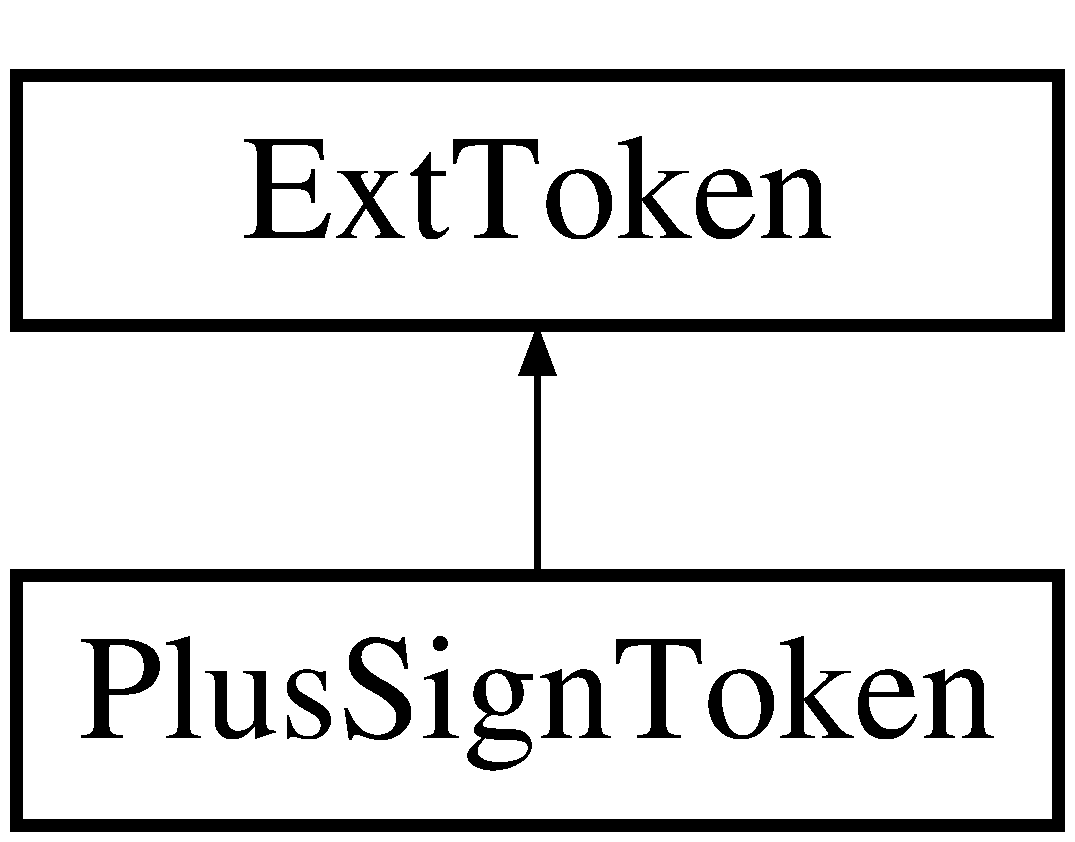
\includegraphics[height=2.000000cm]{classPlusSignToken}
\end{center}
\end{figure}
\subsection*{Public Member Functions}
\begin{DoxyCompactItemize}
\item 
\hypertarget{classPlusSignToken_ad480457c426f911f8286a73e8cf7f949}{{\bfseries Plus\-Sign\-Token} (\hyperlink{classParser}{Parser} $\ast$p, \hyperlink{classToken}{Token} $\ast$t)}\label{classPlusSignToken_ad480457c426f911f8286a73e8cf7f949}

\item 
\hypertarget{classPlusSignToken_a4d79a17891f92800259308ce71402526}{\hyperlink{classParseResult}{Parse\-Result} {\bfseries led} (\hyperlink{classParseResult}{Parse\-Result} left)}\label{classPlusSignToken_a4d79a17891f92800259308ce71402526}

\item 
\hypertarget{classPlusSignToken_a61a05ac9660848e13da97d5746808868}{std\-::string {\bfseries description} ()}\label{classPlusSignToken_a61a05ac9660848e13da97d5746808868}

\item 
\hypertarget{classPlusSignToken_a80753eec970928e042da350df83150f2}{int {\bfseries lbp} ()}\label{classPlusSignToken_a80753eec970928e042da350df83150f2}

\end{DoxyCompactItemize}
\subsection*{Additional Inherited Members}


The documentation for this class was generated from the following file\-:\begin{DoxyCompactItemize}
\item 
ext\-Token.\-h\end{DoxyCompactItemize}

\hypertarget{classPrintStmt}{\section{Print\-Stmt Class Reference}
\label{classPrintStmt}\index{Print\-Stmt@{Print\-Stmt}}
}


\hyperlink{classStmt}{Stmt} \-:\-:= 'print' '(' \hyperlink{classExpr}{Expr} ')' ';'.  




{\ttfamily \#include $<$A\-S\-T.\-h$>$}

Inheritance diagram for Print\-Stmt\-:\begin{figure}[H]
\begin{center}
\leavevmode
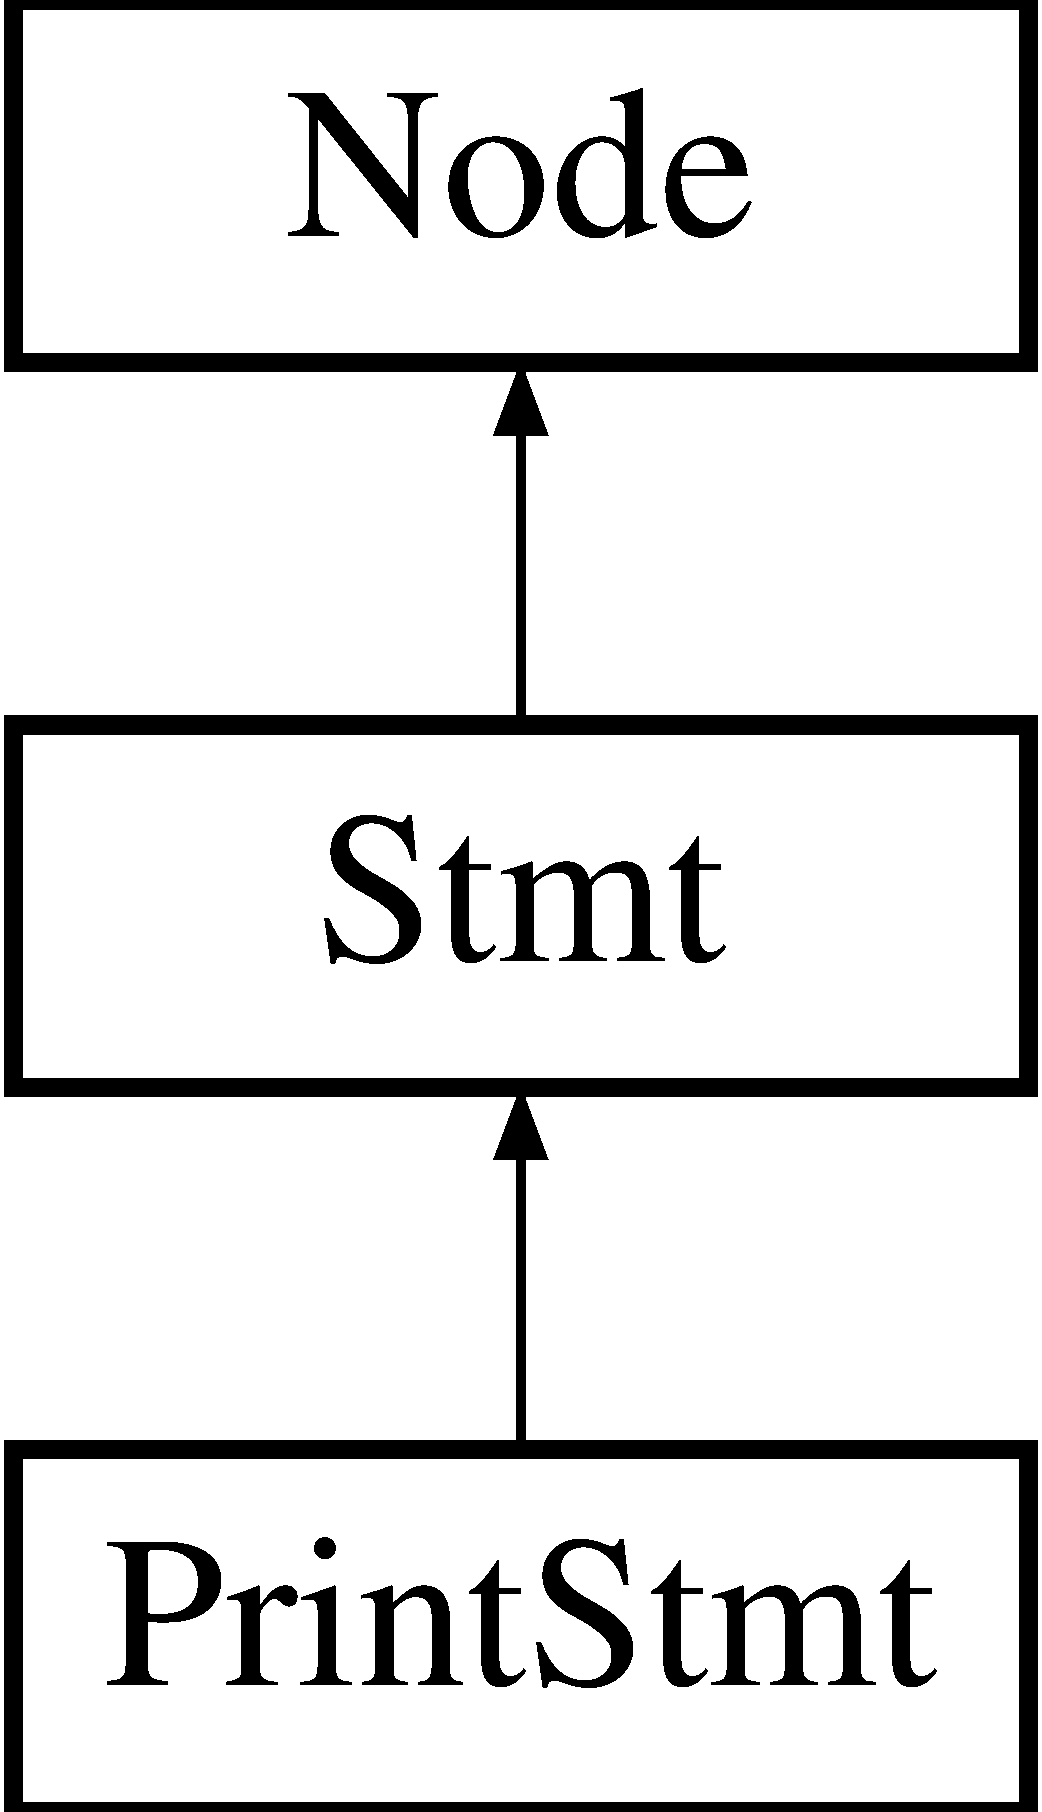
\includegraphics[height=3.000000cm]{classPrintStmt}
\end{center}
\end{figure}
\subsection*{Public Member Functions}
\begin{DoxyCompactItemize}
\item 
\hypertarget{classPrintStmt_a58af5b7c49ef63dfa35950ac253f81ca}{{\bfseries Print\-Stmt} (\hyperlink{classExpr}{Expr} $\ast$e)}\label{classPrintStmt_a58af5b7c49ef63dfa35950ac253f81ca}

\item 
\hypertarget{classPrintStmt_aa3c9ad246b75bd45a48e563500b5109f}{std\-::string \hyperlink{classPrintStmt_aa3c9ad246b75bd45a48e563500b5109f}{unparse} ()}\label{classPrintStmt_aa3c9ad246b75bd45a48e563500b5109f}

\begin{DoxyCompactList}\small\item\em Unparse in proper 'print' form as denoted in grammar. \end{DoxyCompactList}\end{DoxyCompactItemize}


\subsection{Detailed Description}
\hyperlink{classStmt}{Stmt} \-:\-:= 'print' '(' \hyperlink{classExpr}{Expr} ')' ';'. 

The documentation for this class was generated from the following file\-:\begin{DoxyCompactItemize}
\item 
A\-S\-T.\-h\end{DoxyCompactItemize}

\hypertarget{classProgram}{\section{Program Class Reference}
\label{classProgram}\index{Program@{Program}}
}


\hyperlink{classProgram}{Program} \-:\-:= var\-Name '(' ')' '\{' \hyperlink{classStmts}{Stmts} '\}'.  




{\ttfamily \#include $<$A\-S\-T.\-h$>$}

Inheritance diagram for Program\-:\begin{figure}[H]
\begin{center}
\leavevmode
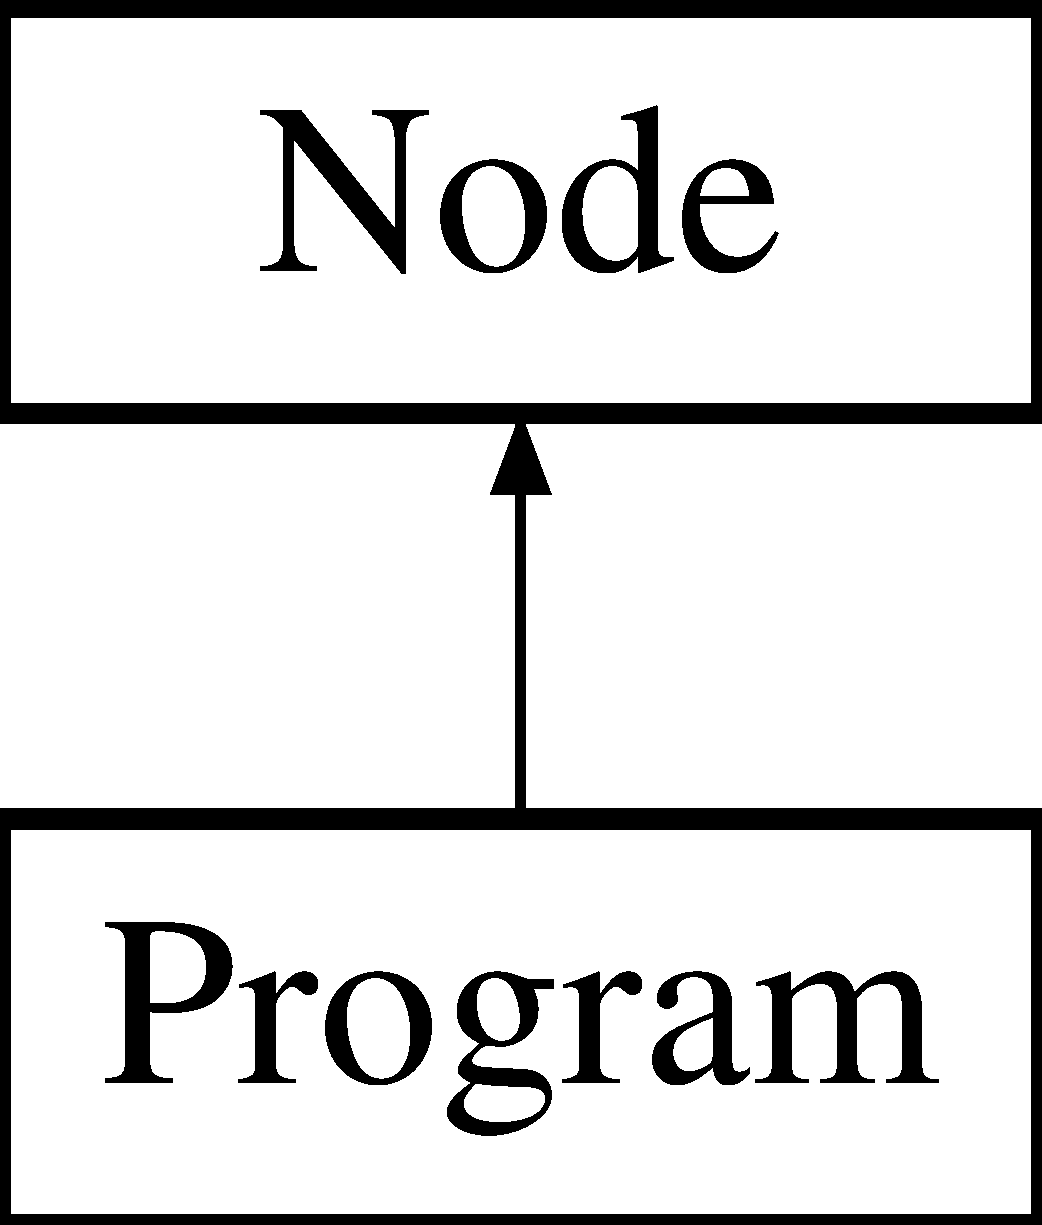
\includegraphics[height=2.000000cm]{classProgram}
\end{center}
\end{figure}
\subsection*{Public Member Functions}
\begin{DoxyCompactItemize}
\item 
\hypertarget{classProgram_aeacce1b9b363aaacb55a074e46a3dd5a}{{\bfseries Program} (\hyperlink{classVarName}{Var\-Name} $\ast$v, \hyperlink{classStmts}{Stmts} $\ast$s)}\label{classProgram_aeacce1b9b363aaacb55a074e46a3dd5a}

\item 
std\-::string \hyperlink{classProgram_a33c78e36a63c63e5821b7747bec7b644}{unparse} ()
\end{DoxyCompactItemize}


\subsection{Detailed Description}
\hyperlink{classProgram}{Program} \-:\-:= var\-Name '(' ')' '\{' \hyperlink{classStmts}{Stmts} '\}'. 

\subsection{Member Function Documentation}
\hypertarget{classProgram_a33c78e36a63c63e5821b7747bec7b644}{\index{Program@{Program}!unparse@{unparse}}
\index{unparse@{unparse}!Program@{Program}}
\subsubsection[{unparse}]{\setlength{\rightskip}{0pt plus 5cm}std\-::string Program\-::unparse (
\begin{DoxyParamCaption}
{}
\end{DoxyParamCaption}
)\hspace{0.3cm}{\ttfamily [inline]}, {\ttfamily [virtual]}}}\label{classProgram_a33c78e36a63c63e5821b7747bec7b644}
Unparse in the following format\-: varname (e.\-g. 'main') () \{ $<$$<$ code here is handled recursively by stmts unparse $>$$>$ \} 

Reimplemented from \hyperlink{classNode_aeb327c708aa4acd82d0f11a9620f0ae8}{Node}.



The documentation for this class was generated from the following file\-:\begin{DoxyCompactItemize}
\item 
A\-S\-T.\-h\end{DoxyCompactItemize}

\hypertarget{classRegexTestSuite}{\section{Regex\-Test\-Suite Class Reference}
\label{classRegexTestSuite}\index{Regex\-Test\-Suite@{Regex\-Test\-Suite}}
}
Inheritance diagram for Regex\-Test\-Suite\-:\begin{figure}[H]
\begin{center}
\leavevmode
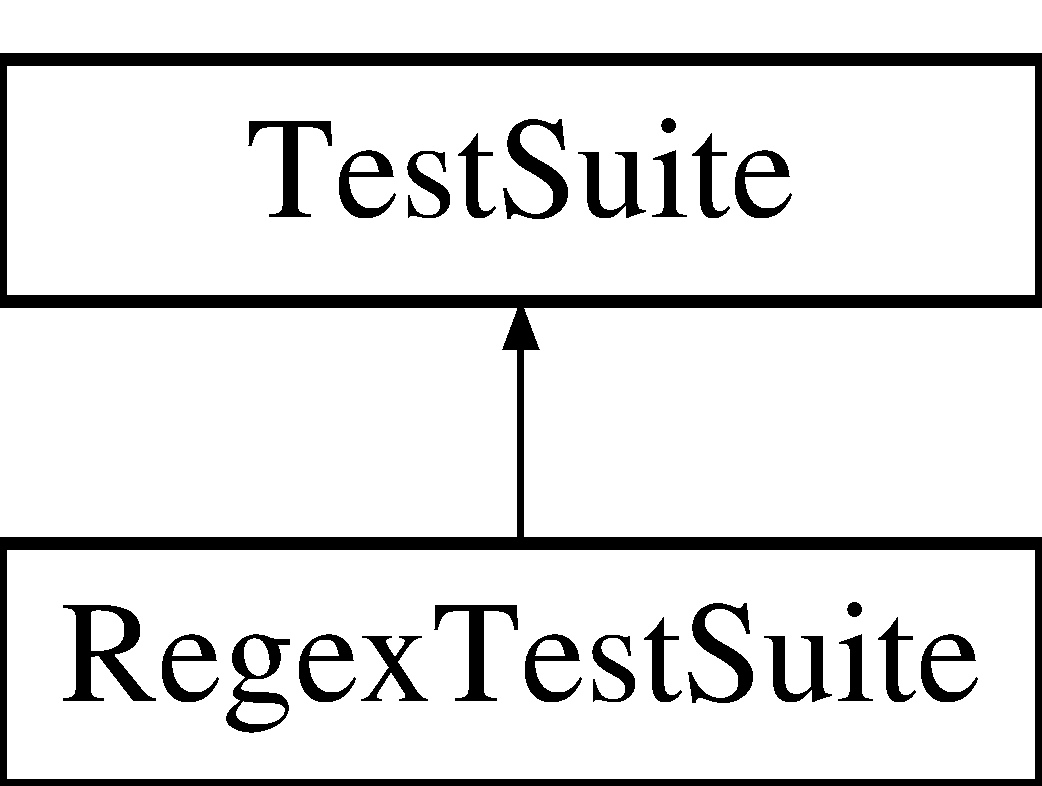
\includegraphics[height=2.000000cm]{classRegexTestSuite}
\end{center}
\end{figure}
\subsection*{Public Member Functions}
\begin{DoxyCompactItemize}
\item 
\hypertarget{classRegexTestSuite_aac0838d917fd9fd6cc71ee086c644555}{void {\bfseries test\-\_\-make\-\_\-match\-Regex\-\_\-match} (void)}\label{classRegexTestSuite_aac0838d917fd9fd6cc71ee086c644555}

\item 
\hypertarget{classRegexTestSuite_ad9c02b9f4fd7feca750d476cda8e0c60}{void {\bfseries test\-\_\-make\-\_\-match\-Regex\-\_\-no\-\_\-match} (void)}\label{classRegexTestSuite_ad9c02b9f4fd7feca750d476cda8e0c60}

\item 
\hypertarget{classRegexTestSuite_a0f46b90e2c0a1c98750a3335d086979a}{void {\bfseries test\-\_\-make\-\_\-match\-Regex\-\_\-match\-\_\-string\-\_\-copy} (void)}\label{classRegexTestSuite_a0f46b90e2c0a1c98750a3335d086979a}

\end{DoxyCompactItemize}


The documentation for this class was generated from the following file\-:\begin{DoxyCompactItemize}
\item 
regex\-\_\-tests.\-h\end{DoxyCompactItemize}

\hypertarget{classRelationalOpToken}{\section{Relational\-Op\-Token Class Reference}
\label{classRelationalOpToken}\index{Relational\-Op\-Token@{Relational\-Op\-Token}}
}
Inheritance diagram for Relational\-Op\-Token\-:\begin{figure}[H]
\begin{center}
\leavevmode
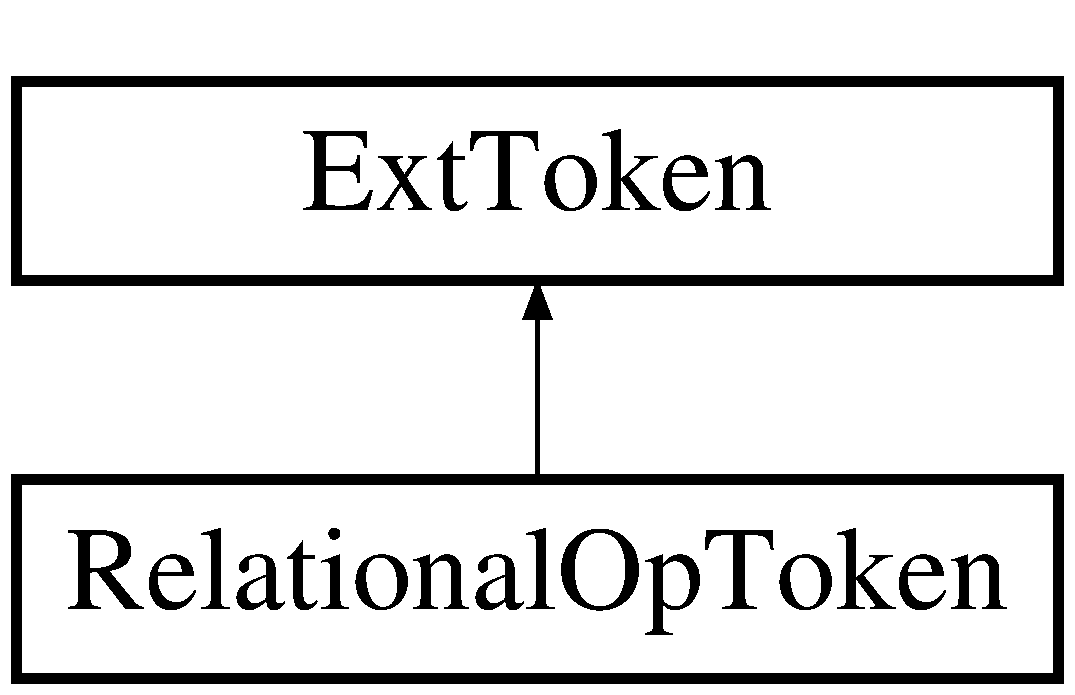
\includegraphics[height=2.000000cm]{classRelationalOpToken}
\end{center}
\end{figure}
\subsection*{Public Member Functions}
\begin{DoxyCompactItemize}
\item 
\hypertarget{classRelationalOpToken_a1ede45cf178138ff12beba209681be51}{{\bfseries Relational\-Op\-Token} (\hyperlink{classParser}{Parser} $\ast$p, \hyperlink{classToken}{Token} $\ast$t, std\-::string d)}\label{classRelationalOpToken_a1ede45cf178138ff12beba209681be51}

\item 
\hypertarget{classRelationalOpToken_a426c64391e7b3272d8e6277964730e05}{\hyperlink{classParseResult}{Parse\-Result} {\bfseries led} (\hyperlink{classParseResult}{Parse\-Result} left)}\label{classRelationalOpToken_a426c64391e7b3272d8e6277964730e05}

\item 
\hypertarget{classRelationalOpToken_ada096491d9553aea21089230489d6aef}{int {\bfseries lbp} ()}\label{classRelationalOpToken_ada096491d9553aea21089230489d6aef}

\end{DoxyCompactItemize}
\subsection*{Additional Inherited Members}


The documentation for this class was generated from the following file\-:\begin{DoxyCompactItemize}
\item 
ext\-Token.\-h\end{DoxyCompactItemize}

\hypertarget{classRepeatStmt}{\section{Repeat\-Stmt Class Reference}
\label{classRepeatStmt}\index{Repeat\-Stmt@{Repeat\-Stmt}}
}


\hyperlink{classStmt}{Stmt} \-:\-:= 'repeat' '(' var\-Name '=' \hyperlink{classExpr}{Expr} 'to' \hyperlink{classExpr}{Expr} ')' \hyperlink{classStmt}{Stmt}.  




{\ttfamily \#include $<$A\-S\-T.\-h$>$}

Inheritance diagram for Repeat\-Stmt\-:\begin{figure}[H]
\begin{center}
\leavevmode
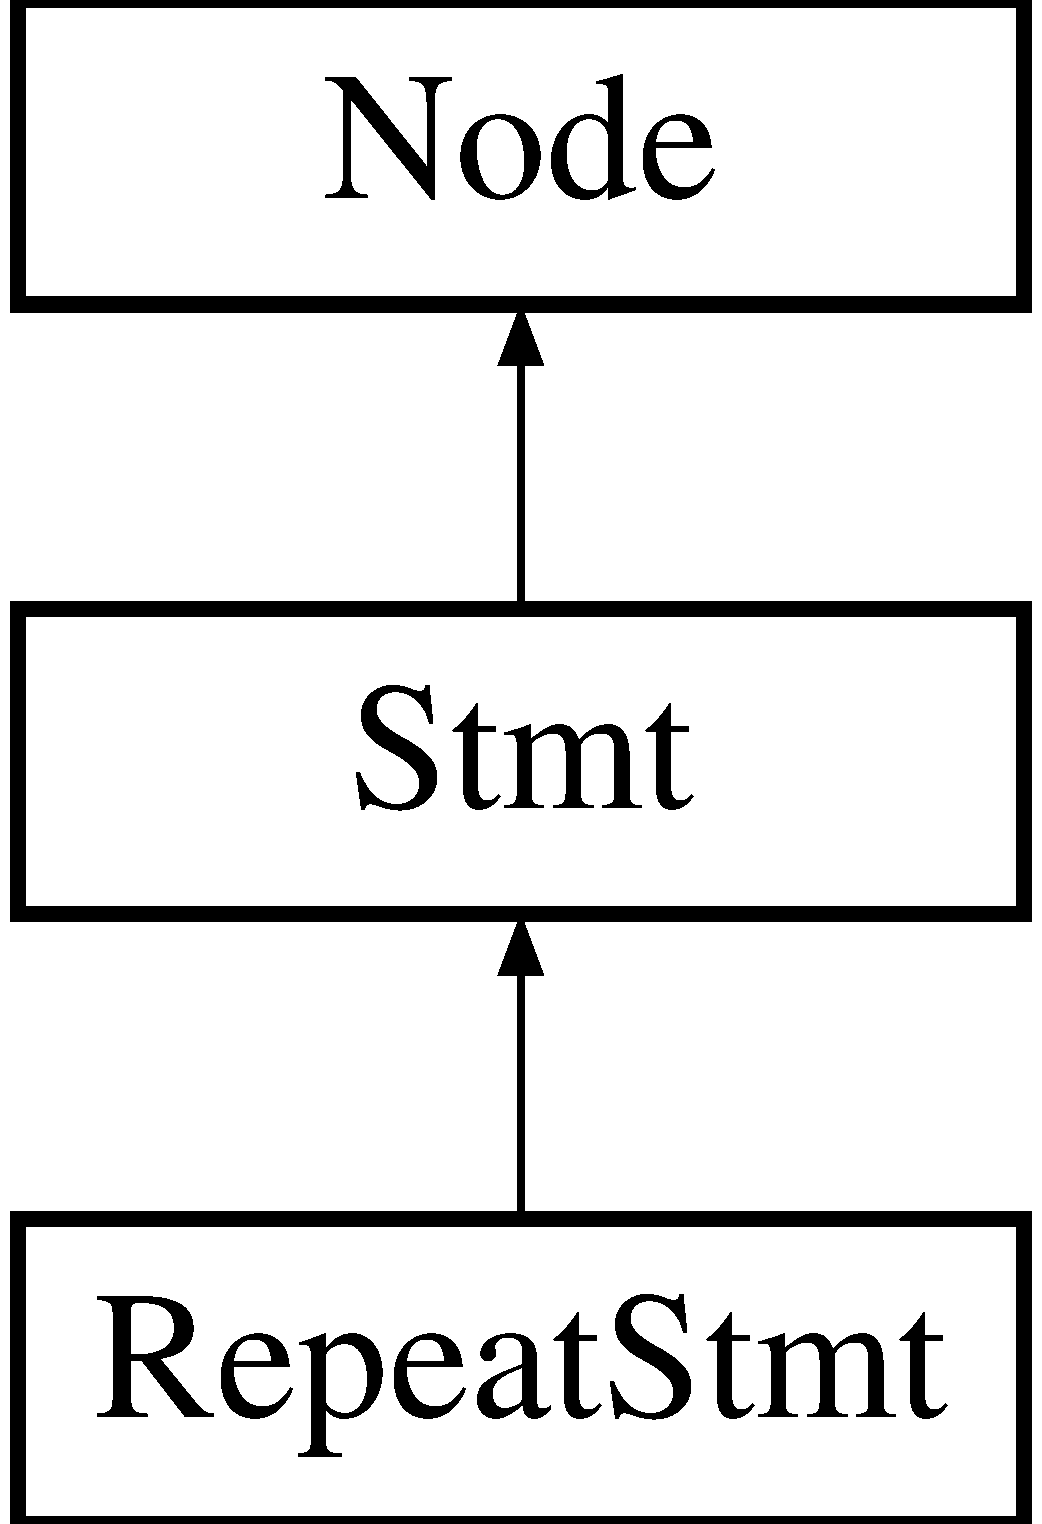
\includegraphics[height=3.000000cm]{classRepeatStmt}
\end{center}
\end{figure}
\subsection*{Public Member Functions}
\begin{DoxyCompactItemize}
\item 
\hypertarget{classRepeatStmt_ad69bc210e4f21f15f34b68522d5aba8f}{{\bfseries Repeat\-Stmt} (std\-::string v, \hyperlink{classExpr}{Expr} $\ast$e1, \hyperlink{classExpr}{Expr} $\ast$e2, \hyperlink{classStmt}{Stmt} $\ast$s)}\label{classRepeatStmt_ad69bc210e4f21f15f34b68522d5aba8f}

\item 
\hypertarget{classRepeatStmt_a9ccc876694fd9b60671818bb9c81447e}{std\-::string \hyperlink{classRepeatStmt_a9ccc876694fd9b60671818bb9c81447e}{unparse} ()}\label{classRepeatStmt_a9ccc876694fd9b60671818bb9c81447e}

\begin{DoxyCompactList}\small\item\em Unparse in proper 'repeat' form as denoted in grammar. \end{DoxyCompactList}\end{DoxyCompactItemize}


\subsection{Detailed Description}
\hyperlink{classStmt}{Stmt} \-:\-:= 'repeat' '(' var\-Name '=' \hyperlink{classExpr}{Expr} 'to' \hyperlink{classExpr}{Expr} ')' \hyperlink{classStmt}{Stmt}. 

The documentation for this class was generated from the following file\-:\begin{DoxyCompactItemize}
\item 
A\-S\-T.\-h\end{DoxyCompactItemize}

\hypertarget{classScanner}{\section{Scanner Class Reference}
\label{classScanner}\index{Scanner@{Scanner}}
}
\subsection*{Public Member Functions}
\begin{DoxyCompactItemize}
\item 
\hypertarget{classScanner_a40f021dac0075b146272e42d425b2ba5}{\hyperlink{classToken}{Token} $\ast$ {\bfseries scan} (const char $\ast$text)}\label{classScanner_a40f021dac0075b146272e42d425b2ba5}

\item 
\hypertarget{classScanner_a38c798b492af63e794c1828d97972e09}{void {\bfseries initialize\-Make\-Regex} ()}\label{classScanner_a38c798b492af63e794c1828d97972e09}

\end{DoxyCompactItemize}
\subsection*{Public Attributes}
\begin{DoxyCompactItemize}
\item 
\hypertarget{classScanner_afc54b08c413bfedb65bd07f6a7f1fe7c}{regex\-\_\-t $\ast$ {\bfseries regex\-Array} \mbox{[}43\mbox{]}}\label{classScanner_afc54b08c413bfedb65bd07f6a7f1fe7c}

\item 
\hypertarget{classScanner_aa60d16396eef75f457036d05e225d23c}{regex\-\_\-t $\ast$ {\bfseries white\-Space}}\label{classScanner_aa60d16396eef75f457036d05e225d23c}

\item 
\hypertarget{classScanner_a00a0ab90d2a971c2d7dc8c14c1baa5ac}{regex\-\_\-t $\ast$ {\bfseries block\-Comment}}\label{classScanner_a00a0ab90d2a971c2d7dc8c14c1baa5ac}

\item 
\hypertarget{classScanner_a338ac417317a864b7236b058ebd02806}{regex\-\_\-t $\ast$ {\bfseries line\-Comment}}\label{classScanner_a338ac417317a864b7236b058ebd02806}

\end{DoxyCompactItemize}


The documentation for this class was generated from the following files\-:\begin{DoxyCompactItemize}
\item 
scanner.\-h\item 
scanner.\-cpp\end{DoxyCompactItemize}

\hypertarget{classScannerTestSuite}{\section{Scanner\-Test\-Suite Class Reference}
\label{classScannerTestSuite}\index{Scanner\-Test\-Suite@{Scanner\-Test\-Suite}}
}
Inheritance diagram for Scanner\-Test\-Suite\-:\begin{figure}[H]
\begin{center}
\leavevmode
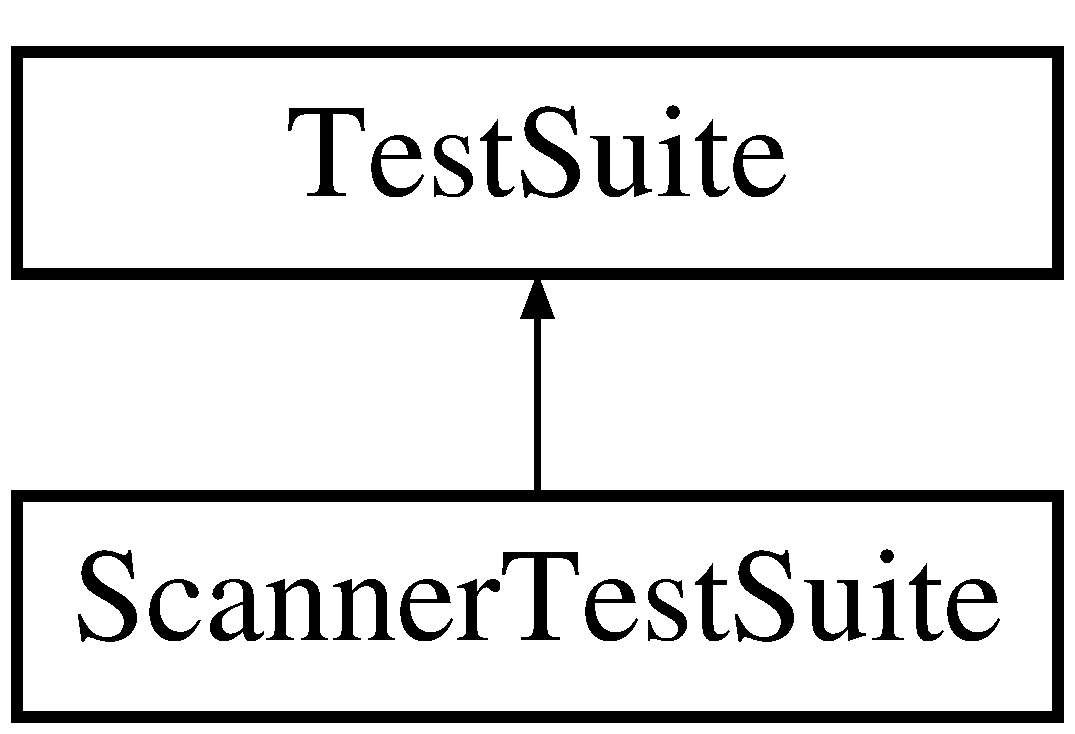
\includegraphics[height=2.000000cm]{classScannerTestSuite}
\end{center}
\end{figure}
\subsection*{Public Member Functions}
\begin{DoxyCompactItemize}
\item 
\hypertarget{classScannerTestSuite_ade832b9b4b3bd92980d43c4050cebd2c}{void {\bfseries test\-\_\-setup\-\_\-code} ()}\label{classScannerTestSuite_ade832b9b4b3bd92980d43c4050cebd2c}

\item 
\hypertarget{classScannerTestSuite_af42f8338bfe7b397ea39f565157f64cc}{void {\bfseries test\-\_\-terminal\-\_\-int\-Kwd} ()}\label{classScannerTestSuite_af42f8338bfe7b397ea39f565157f64cc}

\item 
\hypertarget{classScannerTestSuite_a5c55d99dbc84996abd740fbabb36314b}{void {\bfseries test\-\_\-terminal\-\_\-float\-Kwd} ()}\label{classScannerTestSuite_a5c55d99dbc84996abd740fbabb36314b}

\item 
\hypertarget{classScannerTestSuite_a919ec02392d67e0932affc229b1e72c8}{void {\bfseries test\-\_\-terminal\-\_\-bool\-Kwd} ()}\label{classScannerTestSuite_a919ec02392d67e0932affc229b1e72c8}

\item 
\hypertarget{classScannerTestSuite_a88607da81181c529df9b9edf246dfff6}{void {\bfseries test\-\_\-terminal\-\_\-true\-Kwd} ()}\label{classScannerTestSuite_a88607da81181c529df9b9edf246dfff6}

\item 
\hypertarget{classScannerTestSuite_a6a4395c74f53b0ff0024d6a81999d1b4}{void {\bfseries test\-\_\-terminal\-\_\-false\-Kwd} ()}\label{classScannerTestSuite_a6a4395c74f53b0ff0024d6a81999d1b4}

\item 
\hypertarget{classScannerTestSuite_a141d32b206981d44cbdbf478a20be967}{void {\bfseries test\-\_\-terminal\-\_\-string\-Kwd} ()}\label{classScannerTestSuite_a141d32b206981d44cbdbf478a20be967}

\item 
\hypertarget{classScannerTestSuite_ae2d7798c81ef50444efe99f5c7a89148}{void {\bfseries test\-\_\-terminal\-\_\-matrix\-Kwd} ()}\label{classScannerTestSuite_ae2d7798c81ef50444efe99f5c7a89148}

\item 
\hypertarget{classScannerTestSuite_aa35e7a92f4fdb1b6014ef0ca9df60ecc}{void {\bfseries test\-\_\-terminal\-\_\-let\-Kwd} ()}\label{classScannerTestSuite_aa35e7a92f4fdb1b6014ef0ca9df60ecc}

\item 
\hypertarget{classScannerTestSuite_a1f691532050a3925049694ca6776c08d}{void {\bfseries test\-\_\-terminal\-\_\-in\-Kwd} ()}\label{classScannerTestSuite_a1f691532050a3925049694ca6776c08d}

\item 
\hypertarget{classScannerTestSuite_ae4a9fa8bda3055d8704640f6308a80be}{void {\bfseries test\-\_\-terminal\-\_\-end\-Kwd} ()}\label{classScannerTestSuite_ae4a9fa8bda3055d8704640f6308a80be}

\item 
\hypertarget{classScannerTestSuite_a53ad312be41b5b2e01700f4ef35e3ed2}{void {\bfseries test\-\_\-terminal\-\_\-if\-Kwd} ()}\label{classScannerTestSuite_a53ad312be41b5b2e01700f4ef35e3ed2}

\item 
\hypertarget{classScannerTestSuite_accc9a3822b27c4abeadf5940954df2c6}{void {\bfseries test\-\_\-terminal\-\_\-then\-Kwd} ()}\label{classScannerTestSuite_accc9a3822b27c4abeadf5940954df2c6}

\item 
\hypertarget{classScannerTestSuite_a94ff796af7a2ff4dd70c04615767ab01}{void {\bfseries test\-\_\-terminal\-\_\-else\-Kwd} ()}\label{classScannerTestSuite_a94ff796af7a2ff4dd70c04615767ab01}

\item 
\hypertarget{classScannerTestSuite_a105d4398c5b414a312a6e9b32153dd44}{void {\bfseries test\-\_\-terminal\-\_\-repeat\-Kwd} ()}\label{classScannerTestSuite_a105d4398c5b414a312a6e9b32153dd44}

\item 
\hypertarget{classScannerTestSuite_a9a67154a3d7fd4888e5c4761065a460a}{void {\bfseries test\-\_\-terminal\-\_\-while\-Kwd} ()}\label{classScannerTestSuite_a9a67154a3d7fd4888e5c4761065a460a}

\item 
\hypertarget{classScannerTestSuite_a9c6323869bea7e4c738cedede8abf7a6}{void {\bfseries test\-\_\-terminal\-\_\-print\-Kwd} ()}\label{classScannerTestSuite_a9c6323869bea7e4c738cedede8abf7a6}

\item 
\hypertarget{classScannerTestSuite_a8943aef77dd651d696a879190f199ddb}{void {\bfseries test\-\_\-terminal\-\_\-to\-Kwd} ()}\label{classScannerTestSuite_a8943aef77dd651d696a879190f199ddb}

\item 
\hypertarget{classScannerTestSuite_a6f3d0ce7dbbd7f2a10d5223aa27db46e}{void {\bfseries test\-\_\-terminal\-\_\-int\-Const} ()}\label{classScannerTestSuite_a6f3d0ce7dbbd7f2a10d5223aa27db46e}

\item 
\hypertarget{classScannerTestSuite_a4b66e016244a602826a52db100b3628b}{void {\bfseries test\-\_\-terminal\-\_\-float\-Const} ()}\label{classScannerTestSuite_a4b66e016244a602826a52db100b3628b}

\item 
\hypertarget{classScannerTestSuite_ac6fbb996fdc378700e2c46512d3209e2}{void {\bfseries test\-\_\-terminal\-\_\-string\-Const} ()}\label{classScannerTestSuite_ac6fbb996fdc378700e2c46512d3209e2}

\item 
\hypertarget{classScannerTestSuite_a3a5e102967c53777477ac5205f1e6bdf}{void {\bfseries test\-\_\-terminal\-\_\-variable\-Name1} ()}\label{classScannerTestSuite_a3a5e102967c53777477ac5205f1e6bdf}

\item 
\hypertarget{classScannerTestSuite_a96808ac8cf3e0677c291e1b04e216589}{void {\bfseries test\-\_\-terminal\-\_\-variable\-Name2} ()}\label{classScannerTestSuite_a96808ac8cf3e0677c291e1b04e216589}

\item 
\hypertarget{classScannerTestSuite_a32a17bed3094c2b3a0d2300465e7a3d8}{void {\bfseries test\-\_\-terminal\-\_\-variable\-Name3} ()}\label{classScannerTestSuite_a32a17bed3094c2b3a0d2300465e7a3d8}

\item 
\hypertarget{classScannerTestSuite_ac0e5e742c0384a39833b6f7bc71dd427}{void {\bfseries test\-\_\-terminal\-\_\-left\-Paren} ()}\label{classScannerTestSuite_ac0e5e742c0384a39833b6f7bc71dd427}

\item 
\hypertarget{classScannerTestSuite_afb533b7f05e10c3c5b418738dcac30a1}{void {\bfseries test\-\_\-terminal\-\_\-right\-Paren} ()}\label{classScannerTestSuite_afb533b7f05e10c3c5b418738dcac30a1}

\item 
\hypertarget{classScannerTestSuite_a4db81d5329c9c8d379ddab31626e94ab}{void {\bfseries test\-\_\-terminal\-\_\-left\-Curly} ()}\label{classScannerTestSuite_a4db81d5329c9c8d379ddab31626e94ab}

\item 
\hypertarget{classScannerTestSuite_ae493b914c95d91fdd0bf3119086e1873}{void {\bfseries test\-\_\-terminal\-\_\-right\-Curly} ()}\label{classScannerTestSuite_ae493b914c95d91fdd0bf3119086e1873}

\item 
\hypertarget{classScannerTestSuite_ad203f4631b835998a32530095cbfddf3}{void {\bfseries test\-\_\-terminal\-\_\-left\-Square} ()}\label{classScannerTestSuite_ad203f4631b835998a32530095cbfddf3}

\item 
\hypertarget{classScannerTestSuite_a178af38ac3787ec282cf4a6e471f42f8}{void {\bfseries test\-\_\-terminal\-\_\-right\-Square} ()}\label{classScannerTestSuite_a178af38ac3787ec282cf4a6e471f42f8}

\item 
\hypertarget{classScannerTestSuite_abd07d9b6765ebe5315a3af872de282a4}{void {\bfseries test\-\_\-terminal\-\_\-semi\-Colon} ()}\label{classScannerTestSuite_abd07d9b6765ebe5315a3af872de282a4}

\item 
\hypertarget{classScannerTestSuite_a55c90b619b070f4239bdec72979bb5bf}{void {\bfseries test\-\_\-terminal\-\_\-colon} ()}\label{classScannerTestSuite_a55c90b619b070f4239bdec72979bb5bf}

\item 
\hypertarget{classScannerTestSuite_a8fbf222a7c786640d409c73bec29ee29}{void {\bfseries test\-\_\-terminal\-\_\-assign} ()}\label{classScannerTestSuite_a8fbf222a7c786640d409c73bec29ee29}

\item 
\hypertarget{classScannerTestSuite_a481065e6ca8656159bd055281c0f6823}{void {\bfseries test\-\_\-terminal\-\_\-plus\-Sign} ()}\label{classScannerTestSuite_a481065e6ca8656159bd055281c0f6823}

\item 
\hypertarget{classScannerTestSuite_a4a3dd116effbc9b2b137e847e0018c17}{void {\bfseries test\-\_\-terminal\-\_\-star} ()}\label{classScannerTestSuite_a4a3dd116effbc9b2b137e847e0018c17}

\item 
\hypertarget{classScannerTestSuite_ae4e04072daa5ae9e5372442642d10381}{void {\bfseries test\-\_\-terminal\-\_\-dash} ()}\label{classScannerTestSuite_ae4e04072daa5ae9e5372442642d10381}

\item 
\hypertarget{classScannerTestSuite_ae66a5c2bdbad866169648ead8a16bdbb}{void {\bfseries test\-\_\-terminal\-\_\-forward\-Slash} ()}\label{classScannerTestSuite_ae66a5c2bdbad866169648ead8a16bdbb}

\item 
\hypertarget{classScannerTestSuite_ada7c512cc23c4258c004283f215d0781}{void {\bfseries test\-\_\-terminal\-\_\-less\-Than} ()}\label{classScannerTestSuite_ada7c512cc23c4258c004283f215d0781}

\item 
\hypertarget{classScannerTestSuite_a018c232d0f36ba9096d3608230e20444}{void {\bfseries test\-\_\-terminal\-\_\-less\-Than\-Equal} ()}\label{classScannerTestSuite_a018c232d0f36ba9096d3608230e20444}

\item 
\hypertarget{classScannerTestSuite_ac951625ebf72efa7f3a5c23f7314508f}{void {\bfseries test\-\_\-terminal\-\_\-greater\-Than} ()}\label{classScannerTestSuite_ac951625ebf72efa7f3a5c23f7314508f}

\item 
\hypertarget{classScannerTestSuite_adfcd8e8afce3112198872f54a0ca2c2f}{void {\bfseries test\-\_\-terminal\-\_\-greater\-Than\-Equal} ()}\label{classScannerTestSuite_adfcd8e8afce3112198872f54a0ca2c2f}

\item 
\hypertarget{classScannerTestSuite_a4a15e77f16d68048c1a86ae078be2833}{void {\bfseries test\-\_\-terminal\-\_\-equals\-Equals} ()}\label{classScannerTestSuite_a4a15e77f16d68048c1a86ae078be2833}

\item 
\hypertarget{classScannerTestSuite_ac5ef06e31af6d84f45562beeae37cc0c}{void {\bfseries test\-\_\-terminal\-\_\-not\-Equals} ()}\label{classScannerTestSuite_ac5ef06e31af6d84f45562beeae37cc0c}

\item 
\hypertarget{classScannerTestSuite_ac59bf938e379950259fe3dcd7b49fc8e}{void {\bfseries test\-\_\-terminal\-\_\-and\-Op} ()}\label{classScannerTestSuite_ac59bf938e379950259fe3dcd7b49fc8e}

\item 
\hypertarget{classScannerTestSuite_a419f8b30aa9afc64a53dddac255429c2}{void {\bfseries test\-\_\-terminal\-\_\-or\-Op} ()}\label{classScannerTestSuite_a419f8b30aa9afc64a53dddac255429c2}

\item 
\hypertarget{classScannerTestSuite_a188e5bdd91f633e072957fd4e4944522}{void {\bfseries test\-\_\-terminal\-\_\-not\-Op} ()}\label{classScannerTestSuite_a188e5bdd91f633e072957fd4e4944522}

\item 
\hypertarget{classScannerTestSuite_a92d40fe62e39360d160944ee13d83b81}{void {\bfseries test\-\_\-terminal\-\_\-end\-Of\-File} ()}\label{classScannerTestSuite_a92d40fe62e39360d160944ee13d83b81}

\item 
\hypertarget{classScannerTestSuite_a225e4f3f6647e558afd9733b7a9464e4}{void {\bfseries test\-\_\-terminal\-\_\-lexical\-Error} ()}\label{classScannerTestSuite_a225e4f3f6647e558afd9733b7a9464e4}

\item 
\hypertarget{classScannerTestSuite_a681db679ec2418f862f478fa7678942b}{bool {\bfseries no\-Lexical\-Errors} (\hyperlink{classToken}{Token} $\ast$tks)}\label{classScannerTestSuite_a681db679ec2418f862f478fa7678942b}

\item 
\hypertarget{classScannerTestSuite_a01dc6065a02127accc049627ae234129}{void {\bfseries scan\-File\-No\-Lexical\-Errors} (const char $\ast$filename)}\label{classScannerTestSuite_a01dc6065a02127accc049627ae234129}

\item 
\hypertarget{classScannerTestSuite_a97c50725866b3a5b36c36488053a59bc}{bool {\bfseries same\-Terminals} (\hyperlink{classToken}{Token} $\ast$tks, int num\-Terms, token\-Type $\ast$ts)}\label{classScannerTestSuite_a97c50725866b3a5b36c36488053a59bc}

\item 
\hypertarget{classScannerTestSuite_a01beafb44a33f4d80baf9a4208919c07}{void {\bfseries test\-\_\-scan\-\_\-empty} ()}\label{classScannerTestSuite_a01beafb44a33f4d80baf9a4208919c07}

\item 
\hypertarget{classScannerTestSuite_a304719dd961df0714d372010cdf99ef1}{void {\bfseries test\-\_\-scan\-\_\-empty\-\_\-comment} ()}\label{classScannerTestSuite_a304719dd961df0714d372010cdf99ef1}

\item 
\hypertarget{classScannerTestSuite_af85168e66ba2b924488aca9768231367}{void {\bfseries test\-\_\-scan\-\_\-lexical\-Errors} ()}\label{classScannerTestSuite_af85168e66ba2b924488aca9768231367}

\item 
\hypertarget{classScannerTestSuite_a4bd4d5fc2218f3d28b08b2821ecc271b}{void {\bfseries test\-\_\-scan\-\_\-nums\-\_\-vars} ()}\label{classScannerTestSuite_a4bd4d5fc2218f3d28b08b2821ecc271b}

\item 
\hypertarget{classScannerTestSuite_aad7648d262ef3c103f0792ef73aa3bd8}{void {\bfseries test\-\_\-scan\-\_\-bad\-\_\-syntax\-\_\-good\-\_\-tokens} ()}\label{classScannerTestSuite_aad7648d262ef3c103f0792ef73aa3bd8}

\item 
\hypertarget{classScannerTestSuite_a8248f8bda6c9909971ef13f1364ab8f8}{void {\bfseries test\-\_\-scan\-\_\-sample\-\_\-forest\-Loss} ()}\label{classScannerTestSuite_a8248f8bda6c9909971ef13f1364ab8f8}

\end{DoxyCompactItemize}
\subsection*{Public Attributes}
\begin{DoxyCompactItemize}
\item 
\hypertarget{classScannerTestSuite_a39987f3459098101d7c7fb5a4492996d}{\hyperlink{classScanner}{Scanner} $\ast$ {\bfseries s}}\label{classScannerTestSuite_a39987f3459098101d7c7fb5a4492996d}

\end{DoxyCompactItemize}


The documentation for this class was generated from the following file\-:\begin{DoxyCompactItemize}
\item 
scanner\-\_\-tests.\-h\end{DoxyCompactItemize}

\hypertarget{classSemiColonStmt}{\section{Semi\-Colon\-Stmt Class Reference}
\label{classSemiColonStmt}\index{Semi\-Colon\-Stmt@{Semi\-Colon\-Stmt}}
}


\hyperlink{classStmt}{Stmt} \-:\-:= ';'.  




{\ttfamily \#include $<$A\-S\-T.\-h$>$}

Inheritance diagram for Semi\-Colon\-Stmt\-:\begin{figure}[H]
\begin{center}
\leavevmode
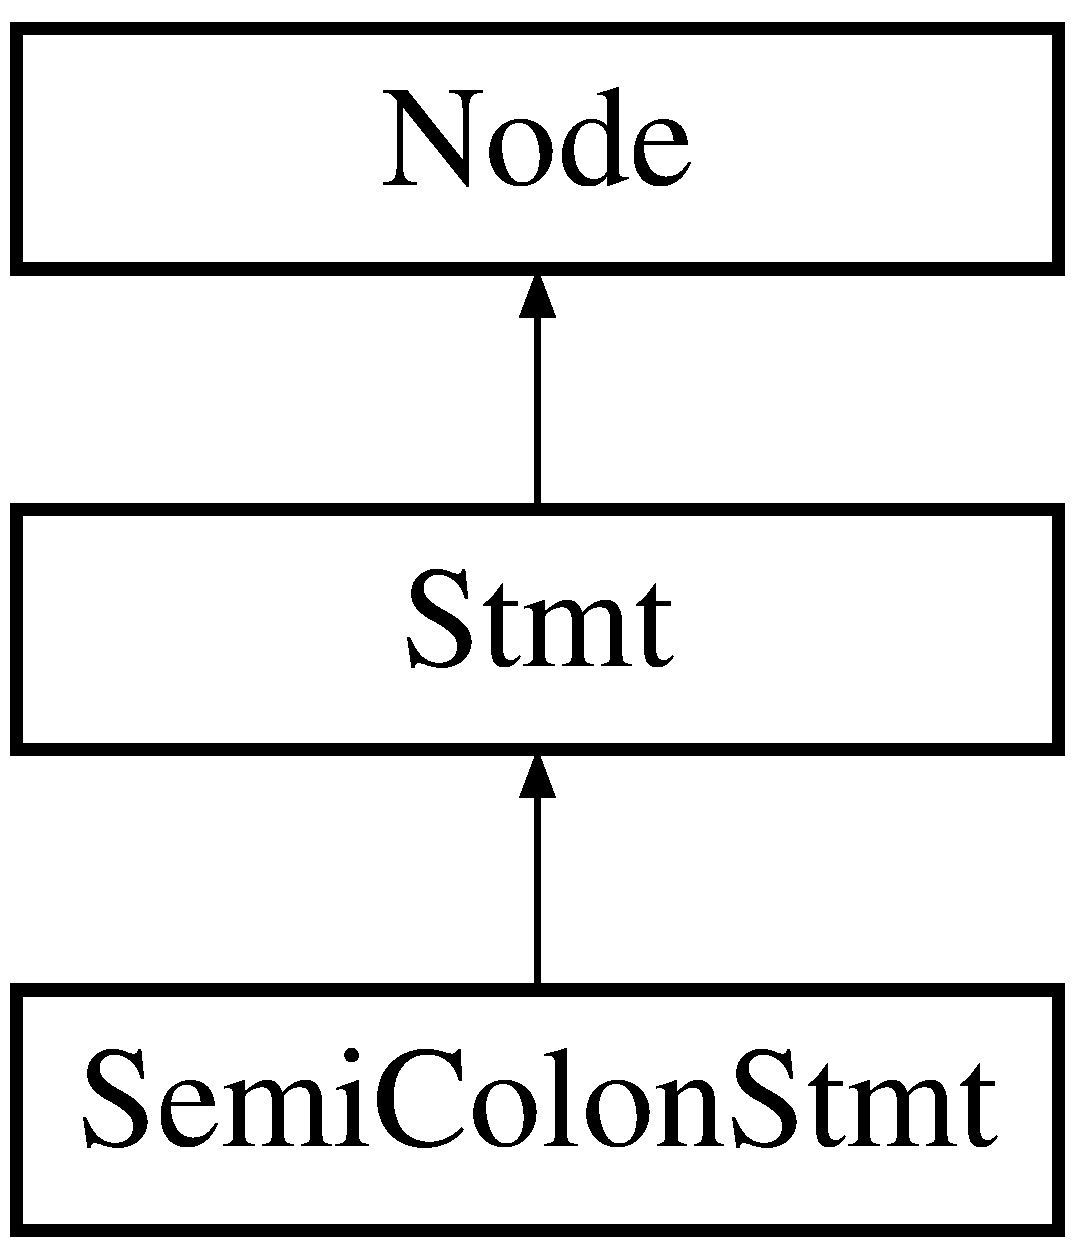
\includegraphics[height=3.000000cm]{classSemiColonStmt}
\end{center}
\end{figure}
\subsection*{Public Member Functions}
\begin{DoxyCompactItemize}
\item 
std\-::string \hyperlink{classSemiColonStmt_a210b082574bda3fa4b408f0022987501}{unparse} ()
\end{DoxyCompactItemize}


\subsection{Detailed Description}
\hyperlink{classStmt}{Stmt} \-:\-:= ';'. 

\subsection{Member Function Documentation}
\hypertarget{classSemiColonStmt_a210b082574bda3fa4b408f0022987501}{\index{Semi\-Colon\-Stmt@{Semi\-Colon\-Stmt}!unparse@{unparse}}
\index{unparse@{unparse}!SemiColonStmt@{Semi\-Colon\-Stmt}}
\subsubsection[{unparse}]{\setlength{\rightskip}{0pt plus 5cm}std\-::string Semi\-Colon\-Stmt\-::unparse (
\begin{DoxyParamCaption}
{}
\end{DoxyParamCaption}
)\hspace{0.3cm}{\ttfamily [inline]}, {\ttfamily [virtual]}}}\label{classSemiColonStmt_a210b082574bda3fa4b408f0022987501}
The unparse method is inherited by each class. This node return should never execute. 

Reimplemented from \hyperlink{classNode_aeb327c708aa4acd82d0f11a9620f0ae8}{Node}.



The documentation for this class was generated from the following file\-:\begin{DoxyCompactItemize}
\item 
A\-S\-T.\-h\end{DoxyCompactItemize}

\hypertarget{classStandardDecl}{\section{Standard\-Decl Class Reference}
\label{classStandardDecl}\index{Standard\-Decl@{Standard\-Decl}}
}


\hyperlink{classDecl}{Decl} \-:\-:= integer\-Kwd var\-Name $\vert$ float\-Kwd var\-Name $\vert$ string\-Kwd var\-Name $\vert$ bool\-Kwd var\-Name.  




{\ttfamily \#include $<$A\-S\-T.\-h$>$}

Inheritance diagram for Standard\-Decl\-:\begin{figure}[H]
\begin{center}
\leavevmode
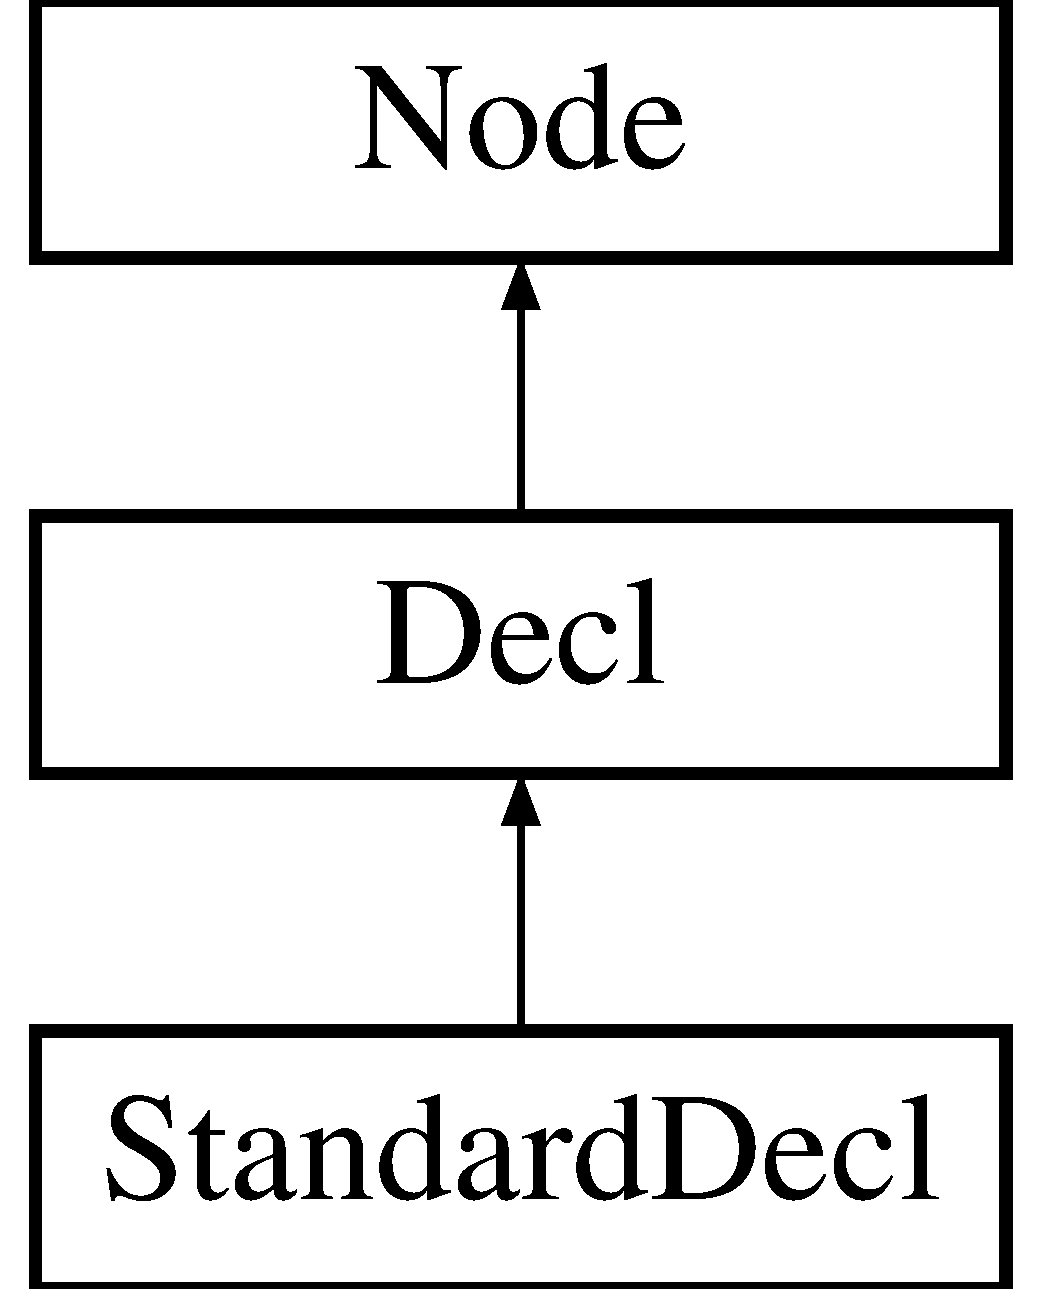
\includegraphics[height=3.000000cm]{classStandardDecl}
\end{center}
\end{figure}
\subsection*{Public Member Functions}
\begin{DoxyCompactItemize}
\item 
\hypertarget{classStandardDecl_ae705d27eabb569629722ae74c4863389}{{\bfseries Standard\-Decl} (std\-::string kwd, std\-::string var\-Name)}\label{classStandardDecl_ae705d27eabb569629722ae74c4863389}

\item 
\hypertarget{classStandardDecl_a2666e01d836103d4a4338a2c54106db5}{std\-::string \hyperlink{classStandardDecl_a2666e01d836103d4a4338a2c54106db5}{unparse} ()}\label{classStandardDecl_a2666e01d836103d4a4338a2c54106db5}

\begin{DoxyCompactList}\small\item\em Unparse standard declaration in format\-: \char`\"{}type var\-Name;\char`\"{}. \end{DoxyCompactList}\end{DoxyCompactItemize}


\subsection{Detailed Description}
\hyperlink{classDecl}{Decl} \-:\-:= integer\-Kwd var\-Name $\vert$ float\-Kwd var\-Name $\vert$ string\-Kwd var\-Name $\vert$ bool\-Kwd var\-Name. 

The documentation for this class was generated from the following file\-:\begin{DoxyCompactItemize}
\item 
A\-S\-T.\-h\end{DoxyCompactItemize}

\hypertarget{classStarToken}{\section{Star\-Token Class Reference}
\label{classStarToken}\index{Star\-Token@{Star\-Token}}
}
Inheritance diagram for Star\-Token\-:\begin{figure}[H]
\begin{center}
\leavevmode
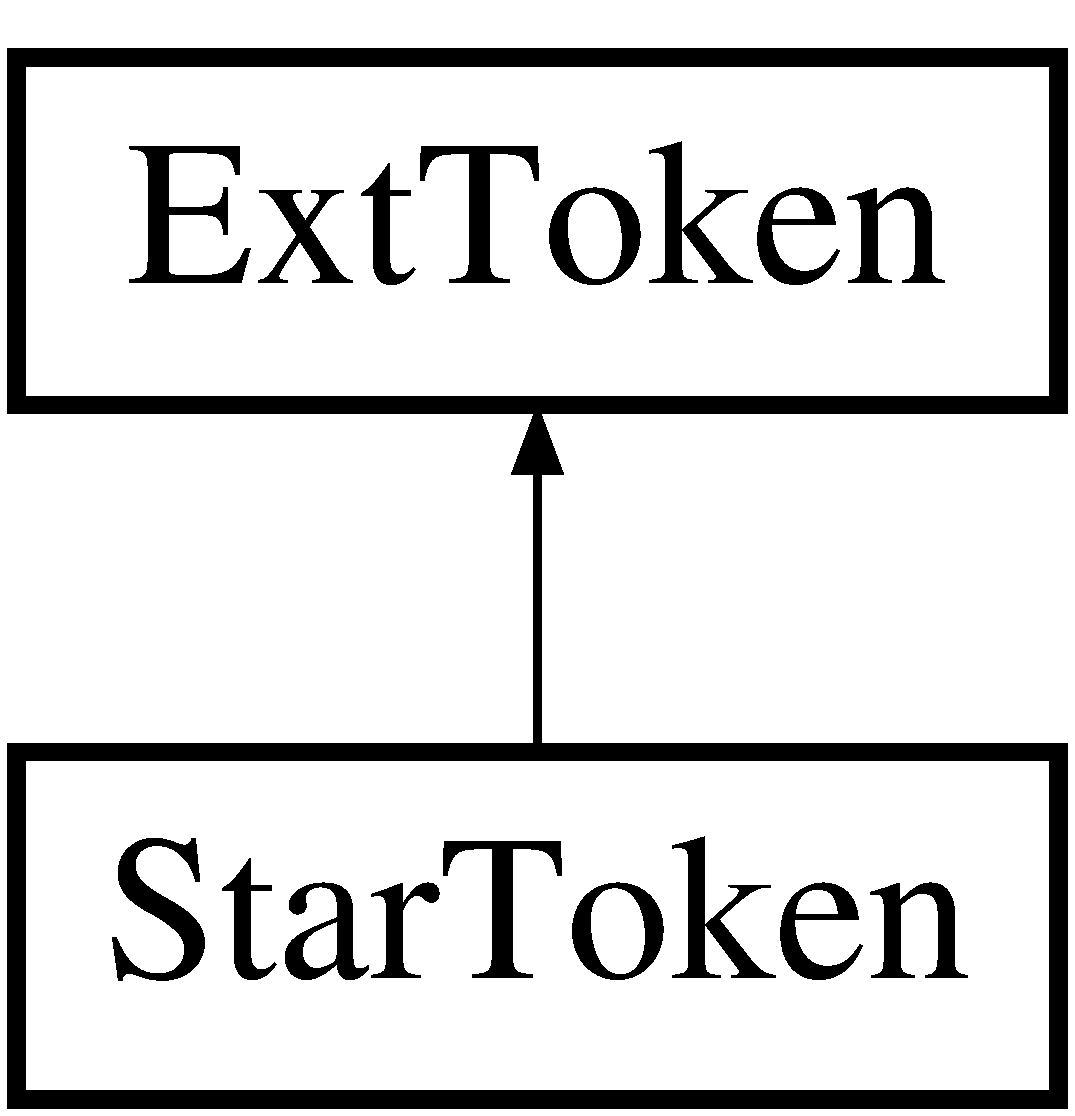
\includegraphics[height=2.000000cm]{classStarToken}
\end{center}
\end{figure}
\subsection*{Public Member Functions}
\begin{DoxyCompactItemize}
\item 
\hypertarget{classStarToken_a9e448a924eb2adbfde602c0590268afd}{{\bfseries Star\-Token} (\hyperlink{classParser}{Parser} $\ast$p, \hyperlink{classToken}{Token} $\ast$t)}\label{classStarToken_a9e448a924eb2adbfde602c0590268afd}

\item 
\hypertarget{classStarToken_aba82bdc81500a58096bfeedad600ad10}{\hyperlink{classParseResult}{Parse\-Result} {\bfseries led} (\hyperlink{classParseResult}{Parse\-Result} left)}\label{classStarToken_aba82bdc81500a58096bfeedad600ad10}

\item 
\hypertarget{classStarToken_a59b81cb08057d75eca4b9a8aad8e2be1}{std\-::string {\bfseries description} ()}\label{classStarToken_a59b81cb08057d75eca4b9a8aad8e2be1}

\item 
\hypertarget{classStarToken_a87682a46d434781795d060e43e7eae23}{int {\bfseries lbp} ()}\label{classStarToken_a87682a46d434781795d060e43e7eae23}

\end{DoxyCompactItemize}
\subsection*{Additional Inherited Members}


The documentation for this class was generated from the following file\-:\begin{DoxyCompactItemize}
\item 
ext\-Token.\-h\end{DoxyCompactItemize}

\hypertarget{classStmt}{\section{Stmt Class Reference}
\label{classStmt}\index{Stmt@{Stmt}}
}
Inheritance diagram for Stmt\-:\begin{figure}[H]
\begin{center}
\leavevmode
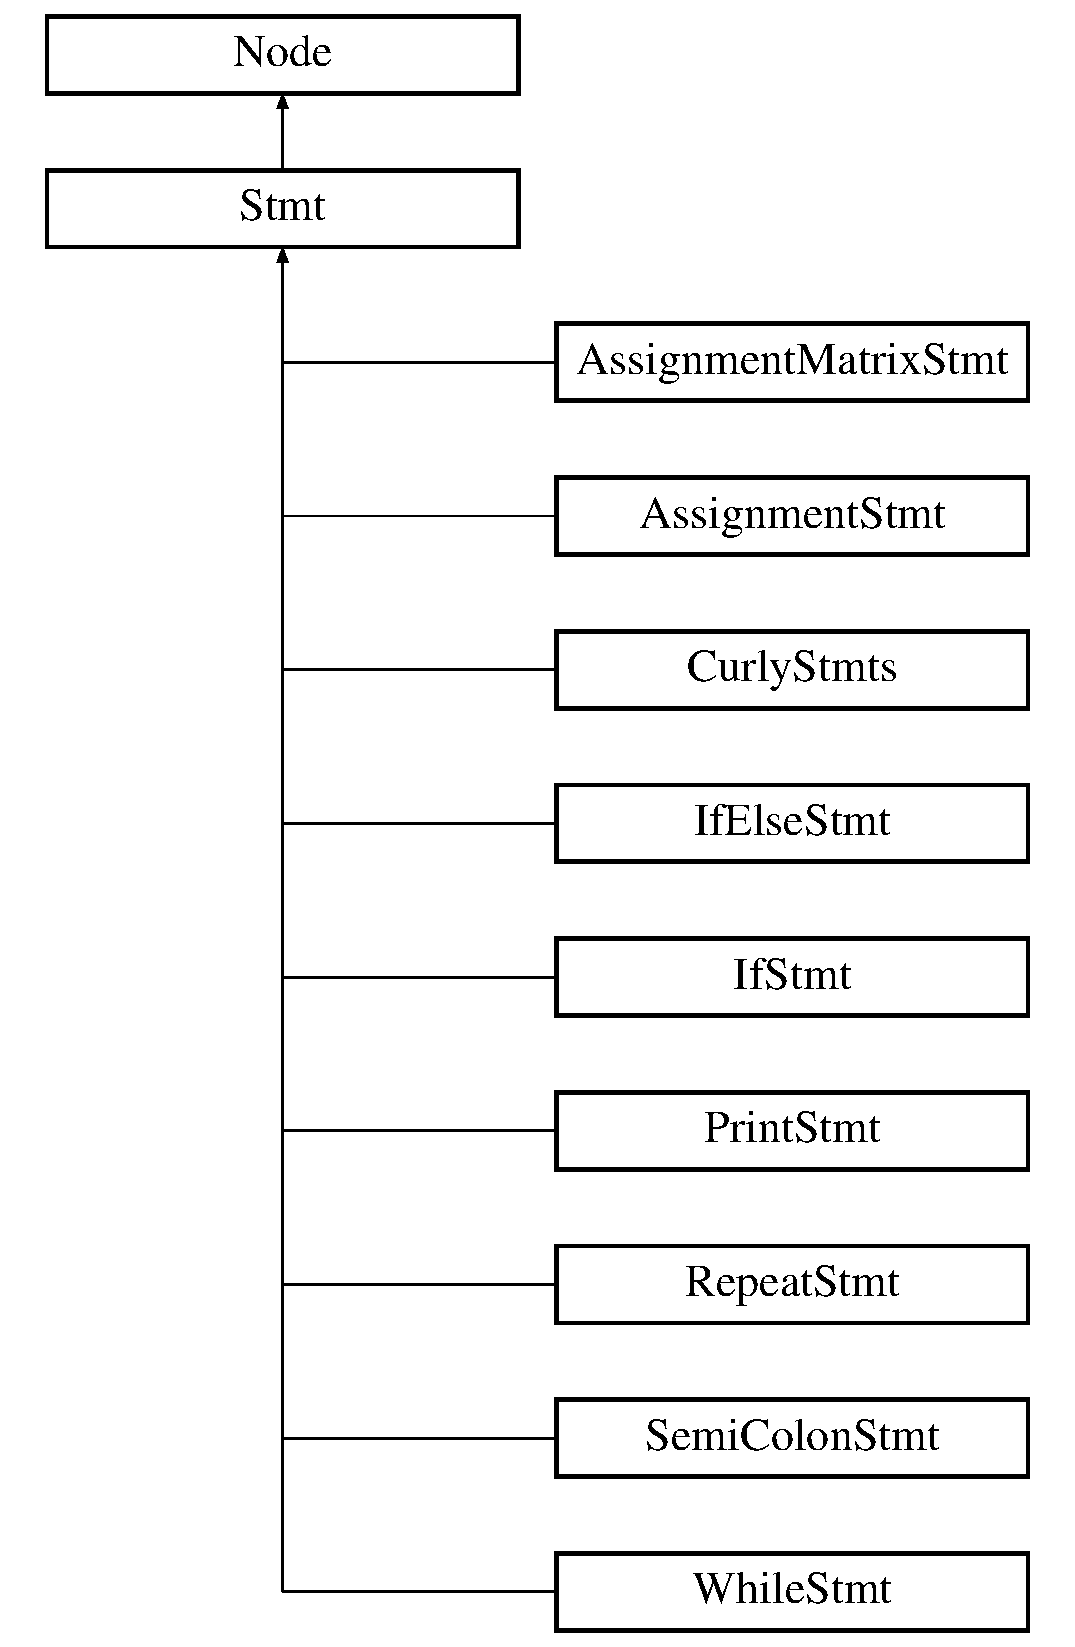
\includegraphics[height=11.000000cm]{classStmt}
\end{center}
\end{figure}
\subsection*{Additional Inherited Members}


The documentation for this class was generated from the following file\-:\begin{DoxyCompactItemize}
\item 
A\-S\-T.\-h\end{DoxyCompactItemize}

\hypertarget{classStmts}{\section{Stmts Class Reference}
\label{classStmts}\index{Stmts@{Stmts}}
}


{\ttfamily \#include $<$A\-S\-T.\-h$>$}

Inheritance diagram for Stmts\-:\begin{figure}[H]
\begin{center}
\leavevmode
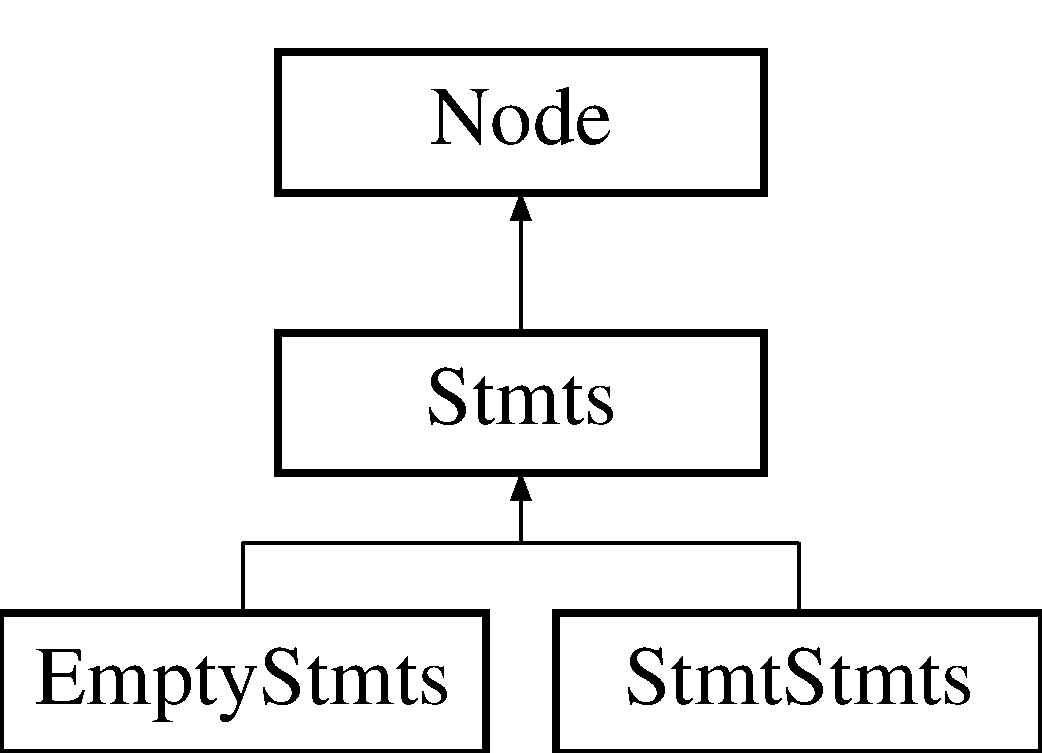
\includegraphics[height=3.000000cm]{classStmts}
\end{center}
\end{figure}
\subsection*{Additional Inherited Members}


\subsection{Detailed Description}
\hyperlink{classStmts}{Stmts}, \hyperlink{classStmt}{Stmt}, \hyperlink{classDecl}{Decl}, \hyperlink{classExpr}{Expr} represent the non-\/terminal types used by our grammar. Each terminal type uses their respective non-\/terminal through inheritance. 

The documentation for this class was generated from the following file\-:\begin{DoxyCompactItemize}
\item 
A\-S\-T.\-h\end{DoxyCompactItemize}

\hypertarget{classStmtStmts}{\section{Stmt\-Stmts Class Reference}
\label{classStmtStmts}\index{Stmt\-Stmts@{Stmt\-Stmts}}
}


{\ttfamily \#include $<$A\-S\-T.\-h$>$}

Inheritance diagram for Stmt\-Stmts\-:\begin{figure}[H]
\begin{center}
\leavevmode
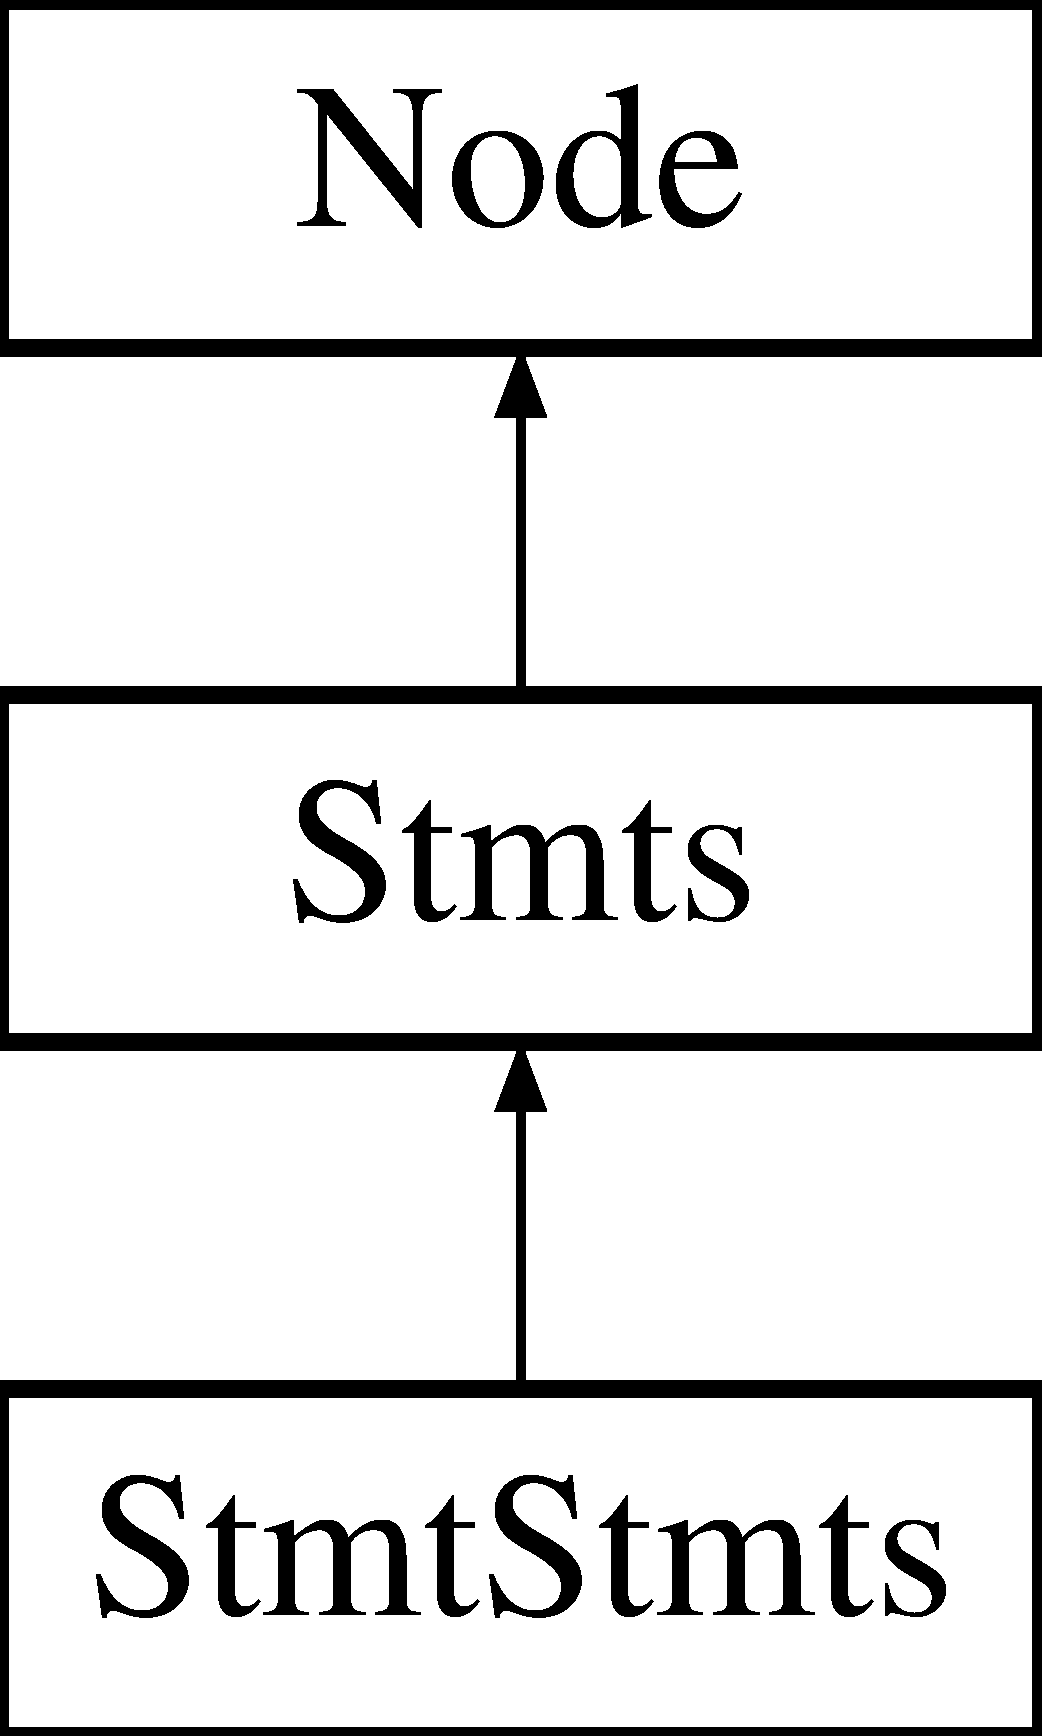
\includegraphics[height=3.000000cm]{classStmtStmts}
\end{center}
\end{figure}
\subsection*{Public Member Functions}
\begin{DoxyCompactItemize}
\item 
\hypertarget{classStmtStmts_aaf6a30cff695500114fda8784a9f4810}{{\bfseries Stmt\-Stmts} (\hyperlink{classStmt}{Stmt} $\ast$s, \hyperlink{classStmts}{Stmts} $\ast$ss)}\label{classStmtStmts_aaf6a30cff695500114fda8784a9f4810}

\item 
\hypertarget{classStmtStmts_a834f10443d4c197b5741a00395f787eb}{std\-::string \hyperlink{classStmtStmts_a834f10443d4c197b5741a00395f787eb}{unparse} ()}\label{classStmtStmts_a834f10443d4c197b5741a00395f787eb}

\begin{DoxyCompactList}\small\item\em Unparses everything recursively between the curly brackets in main () \{ ... \}. \end{DoxyCompactList}\end{DoxyCompactItemize}


\subsection{Detailed Description}
The constructor for stmt\-Stmts is passed pointers for nodes stmt and stmts \hyperlink{classStmts}{Stmts} \-:\-:= \hyperlink{classStmt}{Stmt} \hyperlink{classStmts}{Stmts} 

The documentation for this class was generated from the following file\-:\begin{DoxyCompactItemize}
\item 
A\-S\-T.\-h\end{DoxyCompactItemize}

\hypertarget{classStringConstToken}{\section{String\-Const\-Token Class Reference}
\label{classStringConstToken}\index{String\-Const\-Token@{String\-Const\-Token}}
}
Inheritance diagram for String\-Const\-Token\-:\begin{figure}[H]
\begin{center}
\leavevmode
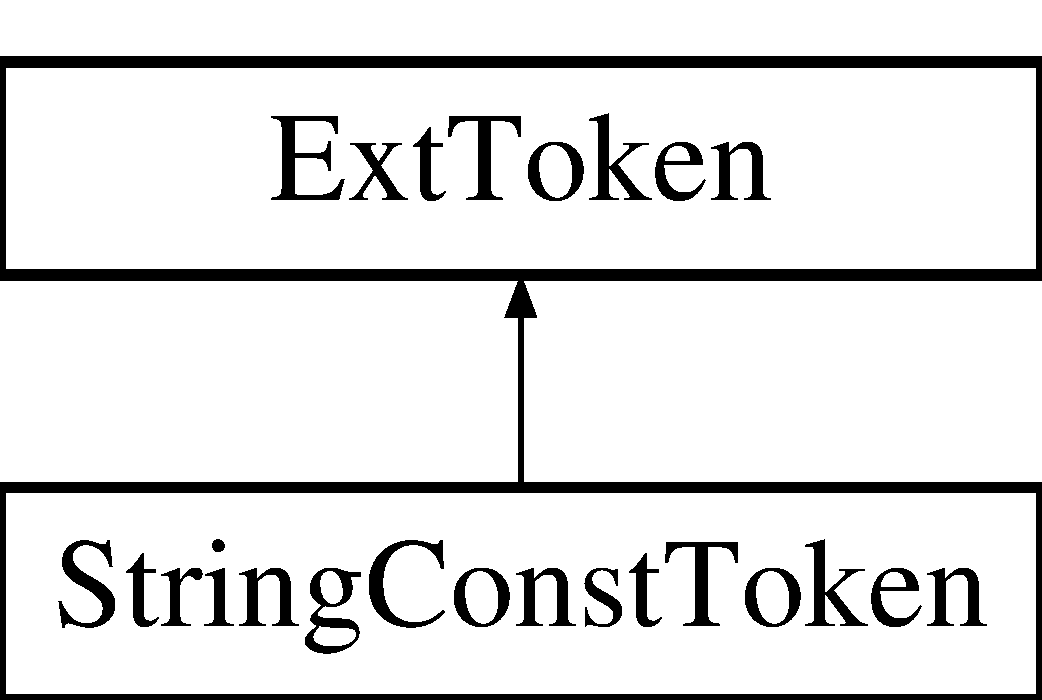
\includegraphics[height=2.000000cm]{classStringConstToken}
\end{center}
\end{figure}
\subsection*{Public Member Functions}
\begin{DoxyCompactItemize}
\item 
\hypertarget{classStringConstToken_aba75cdaef187138a572ba49a5c279fcf}{{\bfseries String\-Const\-Token} (\hyperlink{classParser}{Parser} $\ast$p, \hyperlink{classToken}{Token} $\ast$t)}\label{classStringConstToken_aba75cdaef187138a572ba49a5c279fcf}

\item 
\hypertarget{classStringConstToken_a4767bba84d30289ab31d501f240b80fb}{\hyperlink{classParseResult}{Parse\-Result} {\bfseries nud} ()}\label{classStringConstToken_a4767bba84d30289ab31d501f240b80fb}

\item 
\hypertarget{classStringConstToken_a6343169471a6cb6e422496f2f640691f}{std\-::string {\bfseries description} ()}\label{classStringConstToken_a6343169471a6cb6e422496f2f640691f}

\end{DoxyCompactItemize}
\subsection*{Additional Inherited Members}


The documentation for this class was generated from the following file\-:\begin{DoxyCompactItemize}
\item 
ext\-Token.\-h\end{DoxyCompactItemize}

\hypertarget{classToken}{\section{Token Class Reference}
\label{classToken}\index{Token@{Token}}
}
\subsection*{Public Member Functions}
\begin{DoxyCompactItemize}
\item 
\hypertarget{classToken_a8830d3f87cac295b0d6d8d1405de7f66}{{\bfseries Token} (std\-::string lexeme, token\-Type terminal, \hyperlink{classToken}{Token} $\ast$next)}\label{classToken_a8830d3f87cac295b0d6d8d1405de7f66}

\end{DoxyCompactItemize}
\subsection*{Public Attributes}
\begin{DoxyCompactItemize}
\item 
\hypertarget{classToken_a11b4722b5e4023d234d2017126de378b}{token\-Type {\bfseries terminal}}\label{classToken_a11b4722b5e4023d234d2017126de378b}

\item 
\hypertarget{classToken_abbff29ede445ed4a8520580f12490832}{std\-::string {\bfseries lexeme}}\label{classToken_abbff29ede445ed4a8520580f12490832}

\item 
\hypertarget{classToken_a32f24a25af788c192e5b387dc8d67914}{\hyperlink{classToken}{Token} $\ast$ {\bfseries next}}\label{classToken_a32f24a25af788c192e5b387dc8d67914}

\end{DoxyCompactItemize}


The documentation for this class was generated from the following files\-:\begin{DoxyCompactItemize}
\item 
scanner.\-h\item 
scanner.\-cpp\end{DoxyCompactItemize}

\hypertarget{classTrueKwdToken}{\section{True\-Kwd\-Token Class Reference}
\label{classTrueKwdToken}\index{True\-Kwd\-Token@{True\-Kwd\-Token}}
}
Inheritance diagram for True\-Kwd\-Token\-:\begin{figure}[H]
\begin{center}
\leavevmode
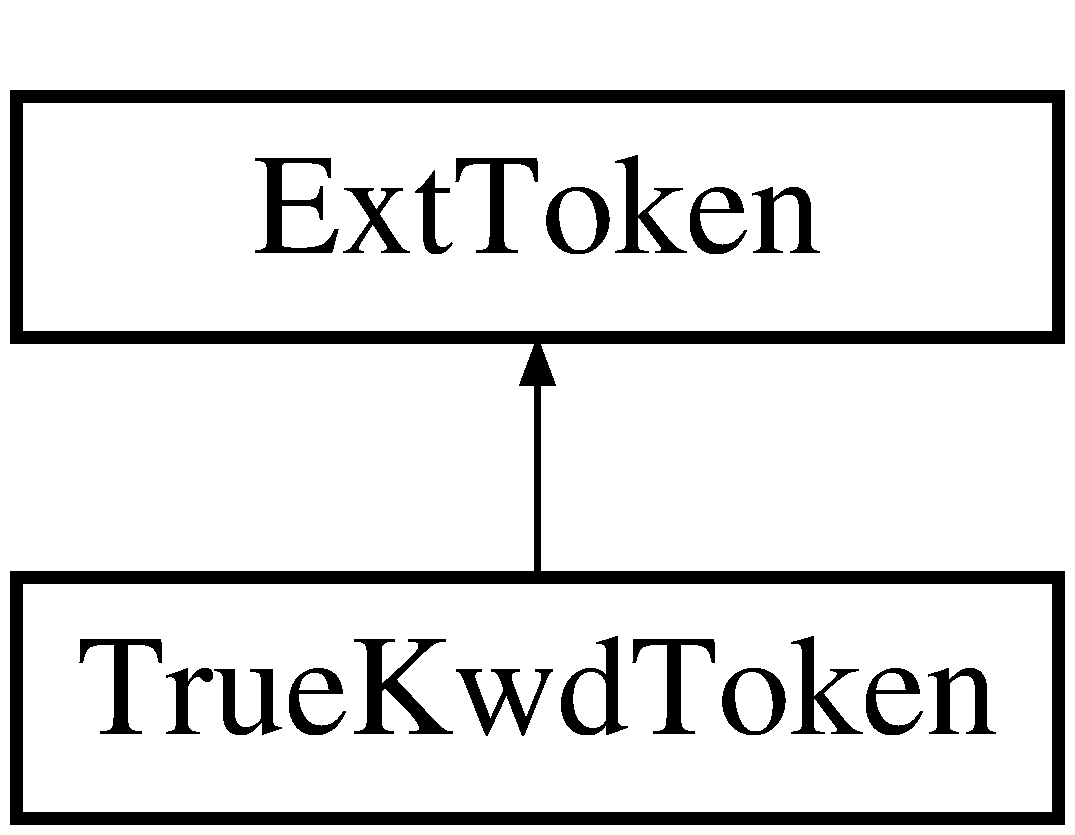
\includegraphics[height=2.000000cm]{classTrueKwdToken}
\end{center}
\end{figure}
\subsection*{Public Member Functions}
\begin{DoxyCompactItemize}
\item 
\hypertarget{classTrueKwdToken_aec070f83a6b91ed35a41e24dfd301b17}{{\bfseries True\-Kwd\-Token} (\hyperlink{classParser}{Parser} $\ast$p, \hyperlink{classToken}{Token} $\ast$t)}\label{classTrueKwdToken_aec070f83a6b91ed35a41e24dfd301b17}

\item 
\hypertarget{classTrueKwdToken_ad86f05acb9483438db153eab44aa6dac}{\hyperlink{classParseResult}{Parse\-Result} {\bfseries nud} ()}\label{classTrueKwdToken_ad86f05acb9483438db153eab44aa6dac}

\item 
\hypertarget{classTrueKwdToken_af4dbe740f06e6928a436d06349af67a9}{std\-::string {\bfseries description} ()}\label{classTrueKwdToken_af4dbe740f06e6928a436d06349af67a9}

\end{DoxyCompactItemize}
\subsection*{Additional Inherited Members}


The documentation for this class was generated from the following file\-:\begin{DoxyCompactItemize}
\item 
ext\-Token.\-h\end{DoxyCompactItemize}

\hypertarget{classTrueOrFalseExpr}{\section{True\-Or\-False\-Expr Class Reference}
\label{classTrueOrFalseExpr}\index{True\-Or\-False\-Expr@{True\-Or\-False\-Expr}}
}


\hyperlink{classExpr}{Expr} \-:\-:= 'true' $\vert$ 'false'.  




{\ttfamily \#include $<$A\-S\-T.\-h$>$}

Inheritance diagram for True\-Or\-False\-Expr\-:\begin{figure}[H]
\begin{center}
\leavevmode
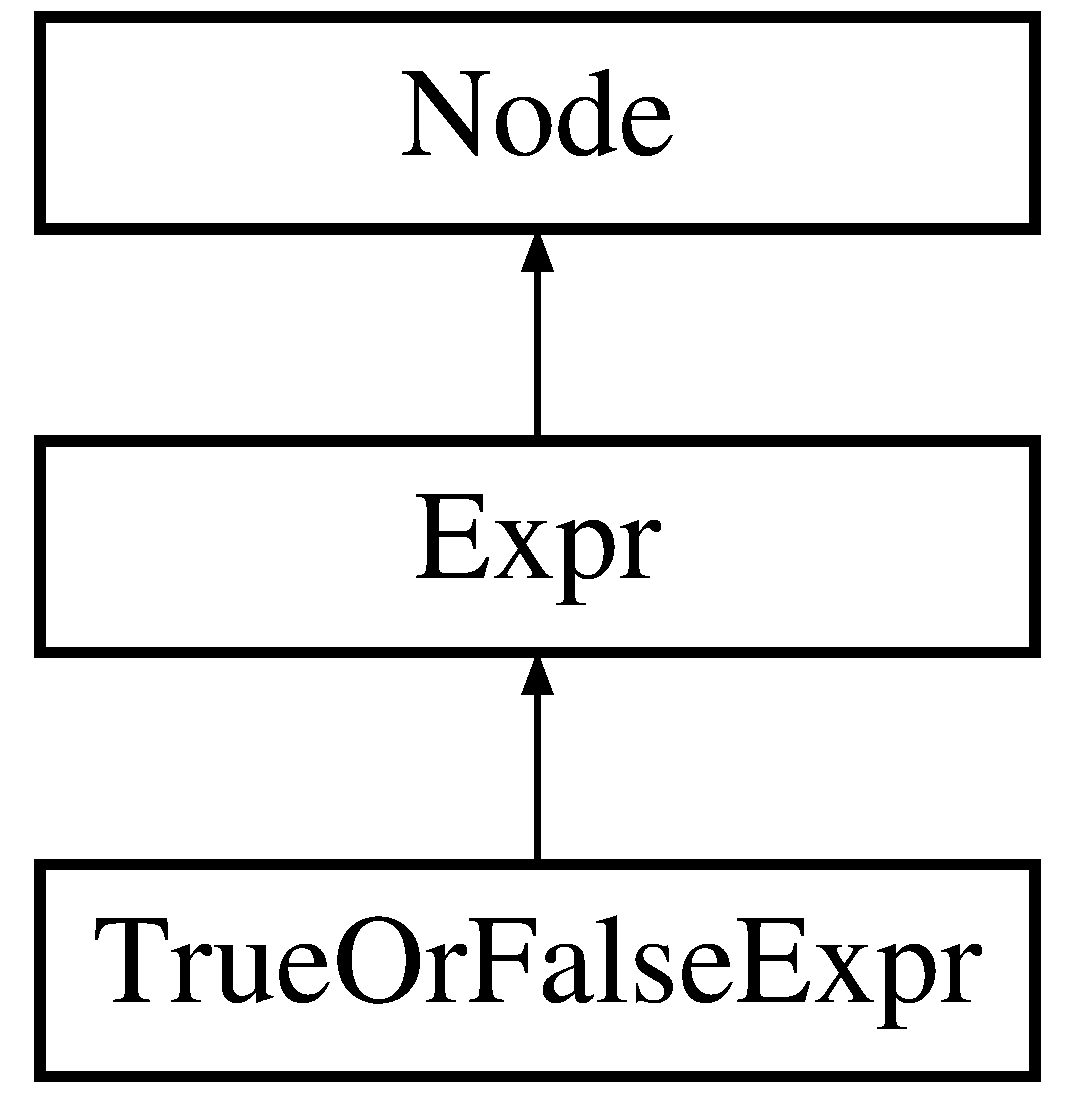
\includegraphics[height=3.000000cm]{classTrueOrFalseExpr}
\end{center}
\end{figure}
\subsection*{Public Member Functions}
\begin{DoxyCompactItemize}
\item 
\hypertarget{classTrueOrFalseExpr_a35003fbd229b0a2a863205119799a36b}{{\bfseries True\-Or\-False\-Expr} (std\-::string trueorfalse)}\label{classTrueOrFalseExpr_a35003fbd229b0a2a863205119799a36b}

\item 
\hypertarget{classTrueOrFalseExpr_a3b981c8f3803f2a2520c7feef1d0ca0b}{std\-::string \hyperlink{classTrueOrFalseExpr_a3b981c8f3803f2a2520c7feef1d0ca0b}{unparse} ()}\label{classTrueOrFalseExpr_a3b981c8f3803f2a2520c7feef1d0ca0b}

\begin{DoxyCompactList}\small\item\em Unparse 'true' or 'false' as a string. \end{DoxyCompactList}\end{DoxyCompactItemize}


\subsection{Detailed Description}
\hyperlink{classExpr}{Expr} \-:\-:= 'true' $\vert$ 'false'. 

The documentation for this class was generated from the following file\-:\begin{DoxyCompactItemize}
\item 
A\-S\-T.\-h\end{DoxyCompactItemize}

\hypertarget{classVariableNameToken}{\section{Variable\-Name\-Token Class Reference}
\label{classVariableNameToken}\index{Variable\-Name\-Token@{Variable\-Name\-Token}}
}
Inheritance diagram for Variable\-Name\-Token\-:\begin{figure}[H]
\begin{center}
\leavevmode
\includegraphics[height=2.000000cm]{classVariableNameToken}
\end{center}
\end{figure}
\subsection*{Public Member Functions}
\begin{DoxyCompactItemize}
\item 
\hypertarget{classVariableNameToken_a804403db425122d1c8d40fd2c6172439}{{\bfseries Variable\-Name\-Token} (\hyperlink{classParser}{Parser} $\ast$p, \hyperlink{classToken}{Token} $\ast$t)}\label{classVariableNameToken_a804403db425122d1c8d40fd2c6172439}

\item 
\hypertarget{classVariableNameToken_a6e775ad5b8c2eafd2e2a185ab90b1f27}{\hyperlink{classParseResult}{Parse\-Result} {\bfseries nud} ()}\label{classVariableNameToken_a6e775ad5b8c2eafd2e2a185ab90b1f27}

\item 
\hypertarget{classVariableNameToken_a54bc3a78736e5c967dc4b1c58e66135b}{std\-::string {\bfseries description} ()}\label{classVariableNameToken_a54bc3a78736e5c967dc4b1c58e66135b}

\end{DoxyCompactItemize}
\subsection*{Additional Inherited Members}


The documentation for this class was generated from the following file\-:\begin{DoxyCompactItemize}
\item 
ext\-Token.\-h\end{DoxyCompactItemize}

\hypertarget{classVarName}{\section{Var\-Name Class Reference}
\label{classVarName}\index{Var\-Name@{Var\-Name}}
}


The \hyperlink{classVarName}{Var\-Name} constructor is passed the string name from prev\-Token-\/$>$lexeme.  




{\ttfamily \#include $<$A\-S\-T.\-h$>$}

Inheritance diagram for Var\-Name\-:\begin{figure}[H]
\begin{center}
\leavevmode
\includegraphics[height=3.000000cm]{classVarName}
\end{center}
\end{figure}
\subsection*{Public Member Functions}
\begin{DoxyCompactItemize}
\item 
\hypertarget{classVarName_afbdf43cec964ba07edee8bdaf2599c28}{\hyperlink{classVarName_afbdf43cec964ba07edee8bdaf2599c28}{Var\-Name} (std\-::string lexeme)}\label{classVarName_afbdf43cec964ba07edee8bdaf2599c28}

\begin{DoxyCompactList}\small\item\em Constructor. \end{DoxyCompactList}\item 
\hypertarget{classVarName_af29612051468cad25343614de9bb067f}{std\-::string \hyperlink{classVarName_af29612051468cad25343614de9bb067f}{unparse} ()}\label{classVarName_af29612051468cad25343614de9bb067f}

\begin{DoxyCompactList}\small\item\em Unparse returns the lexeme of the variable name as a string. \end{DoxyCompactList}\end{DoxyCompactItemize}


\subsection{Detailed Description}
The \hyperlink{classVarName}{Var\-Name} constructor is passed the string name from prev\-Token-\/$>$lexeme. 

The documentation for this class was generated from the following file\-:\begin{DoxyCompactItemize}
\item 
A\-S\-T.\-h\end{DoxyCompactItemize}

\hypertarget{classWhileStmt}{\section{While\-Stmt Class Reference}
\label{classWhileStmt}\index{While\-Stmt@{While\-Stmt}}
}


\hyperlink{classStmt}{Stmt} \-:\-:= 'while' '(' \hyperlink{classExpr}{Expr} ')' \hyperlink{classStmt}{Stmt}.  




{\ttfamily \#include $<$A\-S\-T.\-h$>$}

Inheritance diagram for While\-Stmt\-:\begin{figure}[H]
\begin{center}
\leavevmode
\includegraphics[height=3.000000cm]{classWhileStmt}
\end{center}
\end{figure}
\subsection*{Public Member Functions}
\begin{DoxyCompactItemize}
\item 
\hypertarget{classWhileStmt_a6583cdbdcb6c53a5d0dd0b0c6507ed18}{{\bfseries While\-Stmt} (\hyperlink{classExpr}{Expr} $\ast$e, \hyperlink{classStmt}{Stmt} $\ast$s)}\label{classWhileStmt_a6583cdbdcb6c53a5d0dd0b0c6507ed18}

\item 
\hypertarget{classWhileStmt_acf3bd2eb99735445a3f8b0e2faa27a29}{std\-::string \hyperlink{classWhileStmt_acf3bd2eb99735445a3f8b0e2faa27a29}{unparse} ()}\label{classWhileStmt_acf3bd2eb99735445a3f8b0e2faa27a29}

\begin{DoxyCompactList}\small\item\em Unparse in proper 'while' statement form as denoted in grammar. \end{DoxyCompactList}\end{DoxyCompactItemize}


\subsection{Detailed Description}
\hyperlink{classStmt}{Stmt} \-:\-:= 'while' '(' \hyperlink{classExpr}{Expr} ')' \hyperlink{classStmt}{Stmt}. 

The documentation for this class was generated from the following file\-:\begin{DoxyCompactItemize}
\item 
A\-S\-T.\-h\end{DoxyCompactItemize}

%--- End generated contents ---

% Index
\newpage
\phantomsection
\addcontentsline{toc}{chapter}{Index}
\printindex

\end{document}
